% !TEX root=/home/tavant/these/manuscript/src/manuscript.tex

\documentclass[
   a4paper,	%Pour papier A4
   12pt,		%Taille de la police 12
   twoside,	%recto-verso
   headinclude, headsepline, plainheadsepline,
   bibliography=totoc, toc=listof,
   numbers=noenddot,
   captions=tableheading,
   % fleqn,   % left alignment of formula
   amsmath, hidelinks  ]{book}
   %Packages
% !TEX root=/home/tavant/these/manuscript/src/manuscript.tex

\usepackage[english,french]{babel}

% \usepackage{parskip}  %% Add spaces between paragraphs
% -------------
% font spec
%-----------
\usepackage[T1]{fontenc}

% \usepackage{ebgaramond}

\usepackage{titlesec}
\usepackage{titling}
% Specify different font for section headings
\newcommand*{\headingfont}{\fontfamily{phv}\selectfont}

\titleformat{\chapter}[display]{\Huge\headingfont}{\chaptertitlename\ \thechapter}{20pt}{\Huge}
\titleformat*{\section}{\LARGE\headingfont}
\titleformat*{\subsection}{\Large\headingfont}
\titleformat*{\subsubsection}{\large\headingfont}

%use \showfont to print the current font used
\makeatletter
\newcommand{\showfont}{encoding: \f@encoding{},
  family: \f@family{},
  series: \f@series{},
  shape: \f@shape{},
  size: \f@size{}
}
\newcommand{\iffont}[3]{\ifthenelse{\equal{\f@family}{#1}}{#2}{#3}}
\makeatother



\usepackage{lmodern}% http://ctan.org/pkg/lm for allowing arbitrary font size
\newcommand{\hsc}[1]{{\footnotesize\MakeUppercase{#1}}}   % Fake Small Caps

\usepackage[latin1]{inputenc}
\usepackage{eso-pic}	%eso-pic pour mettre des images avant les chapitres
\usepackage{float, caption}
\usepackage{amsmath,amssymb,mathrsfs,amsfonts}
\usepackage[amssymb,cdot]{SIunits}   %SI units

\usepackage[thmmarks,amsmath]{ntheorem}
\usepackage{array, multirow, tabularx}
\usepackage{mathrsfs}                   %pour faire des cursives dans les formules

\usepackage{listings}		        %Pour ecrire du code
\usepackage[final]{pdfpages}		%Pour insérer des feuilles pdf (page de garde+abstracts)
\usepackage{minitoc} 			%Pour faire des mini tables des matières en début de chapitre

\usepackage{xcolor} %pour avoir les couleurs



\usepackage[nocfg]{nomencl}
\renewcommand{\nomname}{List of Symbols}
\makenomenclature

\usepackage{textcomp} %pour les apostrophes
\usepackage[nottoc,numbib,notlof,notlot]{tocbibind} %pour afficher l'entrée biblio dans la table des matières
%\usepackage[firstpage]{draftwatermark} %pour marquer draft sur la première page
%\SetWatermarkScale{6} %taille de la watermark
%\SetWatermarkLightness{0.9} %transparence de la watermark


% GRAPHICS
\usepackage{graphicx}
\usepackage{subfig}	%pour mettre des subplots


\usepackage{etoolbox}
\patchcmd{\chapter}{plain}{empty}{}{}


\definecolor{lightgray}{gray}{0.95}
\hyphenation{Fortran}		        %Pour eviter l'hyphenation de "Fortran"

\lstset{language=[90]Fortran,	%Pour bien ecrire le code en Fortran
  basicstyle=\fontsize{11}{13}\selectfont\ttfamily,
  keywordstyle=\color{gray},
  commentstyle=\color{blue},
  morecomment=[l]{!\ },  %Comment only with space after !
  captionpos=b, % sets the caption-position to bottom
  frame=single, % adds a frame around the code
  %numbers=left, % where to put the line-numbers
  %numbersep=5pt, % how far the line-numbers are from the code
  %stepnumber=2, % the step between two line-numbers
  rulecolor=\color{black}, % if not set, the frame-color may be changed
  backgroundcolor=\color{lightgray}, % choose the background color
  breaklines=true %break lines if too long
}

% TODO: Fix Greek mu

\usepackage[activate={true,nocompatibility},final,tracking=true,kerning=true,spacing=true,factor=1100,stretch=10,shrink=10]{microtype}
% activate={true,nocompatibility} - activate protrusion and expansion
% final - enable microtype; use "draft" to disable
% tracking=true, kerning=true, spacing=true - activate these techniques
% factor=1100 - add 10% to the protrusion amount (default is 1000)
% stretch=10, shrink=10 - reduce stretchability/shrinkability (default is 20/20)


% For better intext references. By example \cref{fig:X} produces "Fig. n° X" instead of just "X"
\usepackage{varioref} % add the page when the object is far away

\ifpdf
  \usepackage[pagebackref=true,hyperindex=true,colorlinks=true]{hyperref}
  \hypersetup{pdfstartview={FitH}, bookmarksnumbered={true}}

\else
  \usepackage[hypertex=true,hyperindex=true,colorlinks=false]{hyperref}
\fi
\hypersetup{
    colorlinks,
    linkcolor={red!50!black},
    citecolor={blue!50!black},
    urlcolor={blue!80!black}
}

\usepackage[capitalise]{cleveref}  %hance, uyse \vref for the page reference, else \cref only


% For better citations.
\usepackage[numbers]{natbib}
% \usepackage[style=phys]{biblatex}

%~~~~~~~~~~~~~~~~~~~~~~~~~~~~~~
%  Overlay bar for means
\makeatletter
\newsavebox\myboxA
\newsavebox\myboxB
\newlength\mylenA
\usepackage[super]{nth}

\newcommand*\mean[2][0.75]{%
    \sbox{\myboxA}{$\m@th#2$}%
    \setbox\myboxB\null% Phantom box
    \ht\myboxB=\ht\myboxA%
    \dp\myboxB=\dp\myboxA%
    \wd\myboxB=#1\wd\myboxA% Scale phantom
    \sbox\myboxB{$\m@th\overline{\copy\myboxB}$}%  Overlined phantom
    \setlength\mylenA{\the\wd\myboxA}%   calc width diff
    \addtolength\mylenA{-\the\wd\myboxB}%
    \ifdim\wd\myboxB<\wd\myboxA%
       \rlap{\hskip 0.5\mylenA\usebox\myboxB}{\usebox\myboxA}%
    \else
        \hskip -0.5\mylenA\rlap{\usebox\myboxA}{\hskip 0.5\mylenA\usebox\myboxB}%
    \fi}
\makeatother


% !TEX root=/home/tavant/these/manuscript/src/manuscript.tex



\usepackage{xargs}                      % Use more than one optional parameter in a new commands
% \usepackage[pdftex,dvipsnames]{xcolor}  % Coloured text etc.
\usepackage[colorinlistoftodos,prependcaption,textsize=tiny]{todonotes}

\newcommandx{\unsure}[2][1=]{\todo[noline,linecolor=red,backgroundcolor=red!25,bordercolor=red,#1]{#2}}
\newcommandx{\change}[2][1=]{\todo[noline,linecolor=blue,backgroundcolor=blue!25,bordercolor=blue,#1]{#2}}
\newcommandx{\info}[2][1=]{\todo[noline,linecolor=OliveGreen,backgroundcolor=OliveGreen!25,bordercolor=OliveGreen,#1]{#2}}
\newcommandx{\improvement}[2][1=]{\todo[inline,linecolor=red,backgroundcolor=red!25,bordercolor=red,#1]{#2}}
\newcommandx{\thiswillnotshow}[2][1=]{\todo[noline,disable,#1]{#2}}
\newcommandx{\inlinenote}[2][1=]{\todo[inline,size=\small,#1]{#2}}



\usepackage{acronym}  %to handle acronym


% Define the abstract Env.
\usepackage{fancyhdr}
% \pagestyle{fancy}
% \pagestyle{plain}
% \pagestyle{empty}
% \fancyhf{}
% \fancyhead[LE,RO]{Overleaf}
% \fancyhead[RE]{\chaptername}
% \fancyhead[LE]{\thepage}

\newenvironment{abstract}%
    {\cleardoublepage\thispagestyle{empty}\null\vfill\begin{center}%
    \bfseries\abstractname\end{center}}%
    {\vfill\null}


% ignore bibliorapgy if empty
\let\myBib\thebibliography

\renewcommand\thebibliography[1]{\ifx\relax#1\relax\else\myBib{#1}\fi}

%for linebreak
\renewcommand\linebreak{\vspace{1em}}



\newenvironment{zzz}
               {\list{}{\rightmargin0pt \leftmargin4em }%
                \item\relax}
               {\endlist}

\newcommand\subfigurewidth{2.5in}
\newcommand\defaultwidth{4in}

\usepackage[]{algorithm2e}
 \usepackage{mathtools}


 %===================
 % Subfigures
\usepackage[percent]{overpic}
%Floats
\usepackage{placeins}  % allows \FloatBarrier

\newcommand\subfiguretics[3]{
\begin{overpic}[width=\subfigurewidth,grid,tics=10]{#1}
 \put (#3) {\bf #2}
\end{overpic}
}
\newcommand\subfigure[3]{
\begin{overpic}[width=\subfigurewidth]{#1}
 \put (#3) {\bf #2}
\end{overpic}
}


%% table
\usepackage{booktabs}
\newcommand{\ra}[1]{\renewcommand{\arraystretch}{#1}}


%% Fix acronym and cleveref

\makeatletter
% \newcommand*{\org@overidelabel}{}
% \let\org@overridelabel\@verridelabel
% \@ifpackagelater{acronym}{2015/03/21}{% v1.41
%   \renewcommand*{\@verridelabel}[1]{%
%     \@bsphack
%     \protected@write\@auxout{}{\string\AC@undonewlabel{#1@cref}}%
%     \org@overridelabel{#1}%
%     \@esphack
%   }%
% }{% older versions
%   \renewcommand*{\@verridelabel}[1]{%
%     \@bsphack
%     \protected@write\@auxout{}{\string\undonewlabel{#1@cref}}%
%     \org@overridelabel{#1}%
%     \@esphack
%   }%
% }

% 
% \def\@testdef #1#2#3{%
%   \def\reserved@a{#3}\expandafter \ifx \csname #1@#2\endcsname
%  \reserved@a  \else
% \typeout{^^Jlabel #2 changed:^^J%
% \meaning\reserved@a^^J%
% \expandafter\meaning\csname #1@#2\endcsname^^J}%
% \@tempswatrue \fi}
\makeatother



\selectlanguage{english}%

% ===============================
%   INCLUDE
% ===============================
\includeonly{structure/structure,%
 structure/lists,%
 Context/concepts,%
 Chapitre1/1-introduction,%
 Chapitre2/2-mean_values,%
 Chapitre3/3-non_isothermal_sheath%
 }


% !TEX root=/home/tavant/these/manuscript/src/manuscript.tex

%%%%%%%%%%%%%%%%%%%%%%%%%%%%%%%%%%%%%%%%%%%%%%%%%%%%%%%%%%%%%%%%%%%%%%%%%%%%%%%%%%%%%%%%%%%%%%%%%%%%%%%%%%%%%%%%%%%%%%%%%%%%%%%%%%%%%%%%%%%%%%%%%%%%%%%%%%%%%%%%%%%%%%%
%%%%%%%%%%%%%%%%%%%%%%%%%%%%%%%%%%%%%%%%%%%%%%%%%%%%%%%%%%%%%%%%%%%%%%%%%%%%%%%%%%%%%%%%%%%%%%%%%%%%%%%%%%%%%%%%%%%%%%%%%%%%%%%%%%%%%%%%%%%%%%%%%%%%%%%%%%%%%%%%%%%%%%%
%%% Modèle pour la 1ère de couverture des thèses préparées à l'Université Paris-Saclay, basé sur le modèle produit par Guillaume BRIGOT / Template for back cover of thesis made at Université Paris-Saclay, based on the template made by Guillaume BRIGOT
%%% Mis à jour par Aurélien ARNOUX (École polytechnique)/ Updated by Aurélien ARNOUX (École polytechnique)
%%% Les instructions concernant chaque donnée à remplir sont données en bloc de commentaire / Rules to fill this file are given in comment blocks
%%% ATTENTION Ces informations doivent tenir sur une seule page une fois compilées / WARNING These informations must contain in no more than one page once compiled
%%%%%%%%%%%%%%%%%%%%%%%%%%%%%%%%%%%%%%%%%%%%%%%%%%%%%%%%%%%%%%%%%%%%%%%%%%%%%%%%%%%%%%%%%%%%%%%%%%%%%%%%%%%%%%%%%%%%%%%%%%%%%%%%%%%%%%%%%%%%%%%%%%%%%%%%%%%%%%%%%%%%%%%
%%% Version du 19 juillet 2018 (Merci à Hadrien VROYLANDT (Univ. Paris-Sud) pour ses suggestions et corrections)
%%%%%%%%%%%%%%%%%%%%%%%%%%%%%%%%%%%%%%%%%%%%%%%%%%%%%%%%%%%%%%%%%%%%%%%%%%%%%%%%%%%%%%%%%%%%%%%%%%%%%%%%%%%%%%%%%%%%%%%%%%%%%%%%%%%%%%%%%%%%%%%%%%%%%%%%%%%%%%%%%%%%%%%

% \renewcommand{\familydefault}{\sfdefault}
\geometry{
	left=16mm,
	top=30mm,
	right=16mm,
	bottom=30mm
}
\definecolor{bordeau}{rgb}{0.3515625,0,0.234375}

\setlength{\columnseprule}{0pt}
\setlength\columnsep{10pt}


\label{form}
%%%%%%%%%%%%%%%%%%%%%%%%%%%%%%%%%%%%%%%%%%%%%%%%%%%%%%%%%%%%%%%%%%%%%%%%%%%%%%%%%%%%%%%%%%%%%%%%%%%%%%%%%%%%%%%%%%%%%%%%%%%%%%%%%%%%%%%%%%%%%%%%%%%%%%%%%%%%%%%%%%%%%%%
%%%%%%%%%%%%%%%%%%%%%%%%%%%%%%%%%%%%%%%%%%%%%%%%%%%%%%%%%%%%%%%%%%%%%%%%%%%%%%%%%%%%%%%%%%%%%%%%%%%%%%%%%%%%%%%%%%%%%%%%%%%%%%%%%%%%%%%%%%%%%%%%%%%%%%%%%%%%%%%%%%%%%%%
%%% Formulaire / Form
%%% Remplacer les paramètres des \newcommand par les informations demandées / Replace \newcommand parameters by asked informations
%%%%%%%%%%%%%%%%%%%%%%%%%%%%%%%%%%%%%%%%%%%%%%%%%%%%%%%%%%%%%%%%%%%%%%%%%%%%%%%%%%%%%%%%%%%%%%%%%%%%%%%%%%%%%%%%%%%%%%%%%%%%%%%%%%%%%%%%%%%%%%%%%%%%%%%%%%%%%%%%%%%%%%%
%%%%%%%%%%%%%%%%%%%%%%%%%%%%%%%%%%%%%%%%%%%%%%%%%%%%%%%%%%%%%%%%%%%%%%%%%%%%%%%%%%%%%%%%%%%%%%%%%%%%%%%%%%%%%%%%%%%%%%%%%%%%%%%%%%%%%%%%%%%%%%%%%%%%%%%%%%%%%%%%%%%%%%%


\newcommand{\PhDTitle}{Plasma-wall interaction and electron transport in Hall Effect Thrusters} 	%% Titre de la thèse / Thesis title
\newcommand{\PhDname}{Antoine Tavant} 															%% Civilité, nom et prénom /  Civility, first name and name
\newcommand{\NNT}{20XXSACLXXXX} 															%% Numéro National de Thèse (donnée par la bibliothèque à la suite du 1er dépôt)/ National Thesis Number (given by the Library after the first deposit)

\newcommand{\ecodoctitle}{Ondes et Matière} 													%% Nom de l'ED. Voir site de l'Université Paris-Saclay / Full name of Doctoral School. See Université Paris-Saclay website
\newcommand{\ecodocacro}{EDOM}																%% Sigle de l'ED. Voir site de l'Université Paris-Saclay / Acronym of the Doctoral School. See Université Paris-Saclay website
\newcommand{\ecodocnum}{572} 																%% Numéro de l'école doctorale / Doctoral School number
\newcommand{\PhDspeciality}{Physique des Plasmas} 										%% Spécialité de doctorat / Speciality
\newcommand{\PhDworkingplace}{l'École polytechnique} 										%% Établissement de préparation / PhD working place \string: l'Université Paris-Sud, l'Université de Versailles-Saint-Quentin-en-Yvelines, l'Université d'Evry-Val-d'Essonne, l'Institut des sciences et industries du vivant et de l'environnement (AgroParisTech), CentraleSupélec,l'Ecole normale supérieure de Cachan, l'Ecole Polytechnique, l'Ecole nationale supérieure de techniques avancées, l'Ecole nationale de la statistique et de l’administration économique, HEC Paris, l'Institut d'optique théorique et appliquée, Télécom ParisTech, Télécom SudParis
\newcommand{\defenseplace}{Palaiseau} 											%% Ville de soutenance / Place of defense
\newcommand{\defensedate}{18 décembre 2019} 															%% Date de soutenance / Date of defense

%%% Établissement / Institution
%%% Si la thèse a été produite dans le cadre d'une co-tutelle, commenter la partie "Pas de co-tutelle" et décommenter la partie "Co-tutelle" / If the thesis has been prepared in guardianship, comment the part "Pas de co-tutelle" and uncomment the part "Co-tutelle"

	%%%%%%%%%%%%%%%%%%%%%%%%%
	%%% Pas de co-tutelle %%%
	%%%%%%%%%%%%%%%%%%%%%%%%%

\newcommand{\logoEtt}{blank}																%% NE PAS MODIFIER / DO NOT MODIFY
\newcommand{\vpostt}{0.1} 																	%% NE PAS MODIFIER / DO NOT MODIFY
\newcommand{\hpostt}{6}																		%% NE PAS MODIFIER / DO NOT MODIFY
\newcommand{\logoEt}{X} 																	%% Logo de l'établissement de soutenance. Indiquer le sigle / Institution logo. Indicate the acronym \string: AGRO, CENTSUP, ENS, ENSAE, ENSTA, HEC, IOGS, TPT, TSP, UEVE, UPSUD, UVSQ, X
\newcommand{\vpos}{0.1}																		%% À modifier au besoin pour aligner le logo verticalement / If needed, modify to align logo vertilcally
\newcommand{\hpos}{11}																		%% À modifier au besoin pour aligner le logo horizontalement / If needed, modify to align logo horizontaly

		%%%%%%%%%%%%%%%%%%
		%%% Co-tutelle %%%
		%%%%%%%%%%%%%%%%%%
%
% \newcommand{\logoEt}{etab} 																%% Logo de l'université partenaire. Placer le fichier .png dans le répertoire '/couvertures/etab' et indiquer le nom du fichier sans l'extension / Logo of partner university. Place the .png file in the directory '/couvertures/etab' and point the file name without the extension
% \newcommand{\vpos}{0.1}																	%% À modifier au besoin pour aligner les logos verticalement / If needed, modify to align logos vertilcally
% \newcommand{\hpos}{11}																		%% À modifier au besoin pour aligner les logos horizontalement / If needed, modify to align logos horizontaly
% \newcommand{\logoEtt}{etab2}  																%% Logo de l'établissement de soutenance. Le nom du fichier correspond au sigle de l'établissement /  Institution logo. Filename correspond to institution acronym \string: AGRO, CENTSUP, ENS, ENSAE, ENSTA, HEC, IOGS, TPT, TSP, UEVE, UPSUD, UVSQ, X
% \newcommand{\vpostt}{0.1} 																	%% À modifier au besoin pour aligner les logos verticalement / If needed, modify to align logos vertilcally
% \newcommand{\hpostt}{6}																	%% À modifier au besoin pour aligner les logos horizontalement / If needed, modify to align logos horizontaly


%%% JURY

% Lors du premier dépôt de la thèse le nom du président n’est pas connu, le choix du président se fait par les membres du Jury juste avant la soutenance. La précision est apportée sur la couverture lors du second dépôt / Choice of the jury's president is made during the defense. Thus, it must be specified only for the second file deposition in ADUM.
% Tous les membres du juty listés doivent avoir été présents lors de la soutenance / All the jury members listed here must have been present during the defense.

%%% Membre n°1 (Président) / Member n°1 (President)
\newcommand{\jurynameA}{Dr. Pere Roca}
\newcommand{\juryadressA}{Dir. de recherche, LPICM)}
\newcommand{\juryroleA}{Examinateur}

%%% Membre n°2 (Rapporteur) / Member n°2 (President)
\newcommand{\jurynameB}{Prof. Achim von Keudell}
\newcommand{\juryadressB}{Professeur, Ruhr-Universitäte Bochum)}
\newcommand{\juryroleB}{Rapporteur}

%%% Membre n°3 (Rapporteur) / Member n°3 (President)
\newcommand{\jurynameC}{Dr. Gwenael Fubiani}
\newcommand{\juryadressC}{Ch. de recherche, LAPLACE / CNRS}
\newcommand{\juryroleC}{Rapporteur}

%%% Membre n°4 (Examinateur) / Member n°4 (President)
\newcommand{\jurynameD}{Dr. Sedina Tsikata}
\newcommand{\juryadressD}{Ch. de recherche, ICARE / CNRS}
\newcommand{\juryroleD}{Examinateur}

%%% Membre n°5 (Directeur de thèse) / Member n°5 (Thesis supervisor)
\newcommand{\jurynameE}{Dr. Anne Bourdon}
\newcommand{\juryadressE}{Dir. de recherche, LPP / CNRS}
\newcommand{\juryroleE}{Directeur de thèse}

%%% Membre n°6 (Co-directeur de thèse) / Member n°6 (Thesis co-supervisor)
\newcommand{\jurynameF}{Dr. Pascal Chabert}
\newcommand{\juryadressF}{Dir. de recherche, LPP / CNRS}
\newcommand{\juryroleF}{Co-directeur de thèse}

%%% Membre n°7 (Invité) / Member n°7 (Guest)
\newcommand{\jurynameG}{Dr. Stephan Zurbach}
\newcommand{\juryadressG}{Ing. expert senior, Safran Aircraft Engines}
\newcommand{\juryroleG}{Invité}

%%% Membre n°8 (Invité) / Member n°8 (Guest)
\newcommand{\jurynameH}{Prénom Nom}
\newcommand{\juryadressH}{Statut, Établissement (Unité de recherche)}
\newcommand{\juryroleH}{Invité}

%% Il est possible d'ajouter des membres supplémentaires selon le même modèle / More jury members can be added according to the same model

\label{layout}
%%%%%%%%%%%%%%%%%%%%%%%%%%%%%%%%%%%%%%%%%%%%%%%%%%%%%%%%%%%%%%%%%%%%%%%%%%%%%%%%%%%%%%%%%%%%%%%%%%%%%%%%%%%%%%%%%%%%%%%%%%%%%%%%%%%%%%%%%%%%%%%%%%%%%%%%%%%%%%%%%%%%%%%
%%%%%%%%%%%%%%%%%%%%%%%%%%%%%%%%%%%%%%%%%%%%%%%%%%%%%%%%%%%%%%%%%%%%%%%%%%%%%%%%%%%%%%%%%%%%%%%%%%%%%%%%%%%%%%%%%%%%%%%%%%%%%%%%%%%%%%%%%%%%%%%%%%%%%%%%%%%%%%%%%%%%%%%
%%% Mise en page / Page layout
%%% NE RIEN MODIFIER EXCEPTÉ LA PARTIE CONCERNANT LE JURY (voir \label{jury}) SI BESOIN / DO NOT MODIFY EXCEPT SECTION CONCERNING JURY (see \label{jury}) IF NEEDED
%%%%%%%%%%%%%%%%%%%%%%%%%%%%%%%%%%%%%%%%%%%%%%%%%%%%%%%%%%%%%%%%%%%%%%%%%%%%%%%%%%%%%%%%%%%%%%%%%%%%%%%%%%%%%%%%%%%%%%%%%%%%%%%%%%%%%%%%%%%%%%%%%%%%%%%%%%%%%%%%%%%%%%%
%%%%%%%%%%%%%%%%%%%%%%%%%%%%%%%%%%%%%%%%%%%%%%%%%%%%%%%%%%%%%%%%%%%%%%%%%%%%%%%%%%%%%%%%%%%%%%%%%%%%%%%%%%%%%%%%%%%%%%%%%%%%%%%%%%%%%%%%%%%%%%%%%%%%%%%%%%%%%%%%%%%%%%%

% Méta-données du PDF / PDF meta-datas
\hypersetup{
	pdfauthor={\PhDname},
	pdfsubject={Ph.D. thesis manuscrit},
	pdftitle={\PhDTitle},
}




\newcommand{\logoEd}{EDOM}																		%% Logo de l'école doctorale. Indiquer le sigle / Doctoral school logo. Indicate the acronym \string: 2MIB; AAIF; ABIES; BIOSIGNE; CBMS; EDMH; EDOM; EDPIF; EDSP; EOBE; INTERFACES; ITFA; PHENIICS; SDSV; SDV; SHS; SMEMAG; SSMMH; STIC
\newcommand{\PhDTitleFR}{titre (en français)}													%% Titre de la thèse en français / Thesis title in french
\newcommand{\keywordsFR}{3 à 6 mots clés}														%% Mots clés en français, séprarés par des , / Keywords in french, separated by ,
\newcommand{\abstractFR}{\lipsum[1-2]}															%% Résumé en français / abstract in french

\newcommand{\PhDTitleEN}{titre (en anglais)}													%% Titre de la thèse en anglais / Thesis title in english
\newcommand{\keywordsEN}{3 à 6 mots clés}														%% Mots clés en anglais, séprarés par des , / Keywords in english, separated by ,
\newcommand{\abstractEN}{\lipsum[1-2]}															%% Résumé en anglais / abstract in english



% !TEX root=/home/tavant/these/manuscript/src/manuscript.tex



%Uncomment next line if AMS fonts required
%\usepackage{iopams}
\newcommand{\estar}{\epsilon^*}
\newcommand{\Te}{\mathrm{T_e}}
\newcommand{\Ts}{\mathrm{T_s}}
\newcommand{\prl}{\parallel}
\newcommand{\sig}{\sigma}
\newcommand{\sigm}{\sigma_{\rm max}}
\newcommand{\sigo}{\sigma_0}
\newcommand{\rate}{\mean{\sigma}}
\newcommand{\ratecr}{\rate_{\rm cr}}
\newcommand{\norm}[1]{\lvert#1\rvert}
\renewcommand{\vec}[1]{{\bf #1}}
\newcommand{\eV}{{\mathrm{\,V}}}
\newcommand{\LPPicname}{{\it LPPic}}
\newcommand{ \red}{\color{red}}
\newcommand{\ek}{\epsilon}

\usepackage{upgreek}
\newcommand{\mus}{\mathrm{\upmu  s}}

\renewcommand{\div}{\nabla \cdot}

\newcommand{\lb}{\left[}
\newcommand{\rb}{\right]}

\newcommand{\lp}{\left(}
\renewcommand{\rp}{\right)}

\newcommand{\dphi}{\Delta \phi}
\newcommand{\mobeffsat}{\mu_{\mathrm{eff}}^{sat}}
\newcommand{\mobeff}{\mu_{\mathrm{eff}}}
\newcommand{\mobcla}{\mu_{\mathrm{classical}}}
\newcommand{\mobpic}{\mu_{\mathrm{PIC}}}
\newcommand{\M}[1]{{\bf M#1}}

\newcommand{\Ee}{{\mathcal{E}_e}}
\newcommand{\Es}{{\mathcal{E}_s}}

\newcommand\Npc{N_{\rm pc}}
\newcommand\Isp{\ensuremath {\rm I_{\rm sp}}}

% 10^number : use as \sn{Value}{Power} for value x 10^Power
\newcommand{\sn}[2]{\ensuremath{{#1}\times 10^{#2}}}


%mean notation. May need an average command as well
%\newcommand{\mean}[1]{{\overline{#1}}}

\newcommand\LPPic{{\sc LPPic} }

\newcommand\dt{\ensuremath{\Delta t} }


\newcommand{\vect}[1]{{\mathbf #1}}
\newcommand{\epsr}{\epsilon_{R}}
\newcommand{\V}{\Omega_{i,j}}
\newcommand{\C}{C_{i,j}}

\newcommand{\grad}{\vect{\nabla}}
\newcommand{\deriv}[2]{\frac{\partial #1}{\partial #2}}

\newcommand{\dx}{\Delta x}
\newcommand{\dy}{\Delta y}

\newcommand{\N}{\ensuremath{\mathcal{N}}}
\newcommand\stdconv{\ensuremath{\sigma_{\rm Reinj}}}
\newcommand{\aziE}{ {\ensuremath{E_{\theta}}}}
\newcommand\FFT{\ensuremath{ \mathcal{FFT}}}
\newcommand\FT{\ensuremath{ \mathcal{FT}}}

%========================
% Nomenclature

%% This code creates the groups
% -----------------------------------------
\usepackage{etoolbox}
\renewcommand\nomgroup[1]{%
  \item[\bfseries
  \ifstrequal{#1}{P}{Physics Constants}{%
  \ifstrequal{#1}{N}{Number Sets}{%
  \ifstrequal{#1}{Q}{Quantities}{}}}%
]}

% This will add the units
%----------------------------------------------
\newcommand{\nomunit}[1]{%
\renewcommand{\nomentryend}{\hspace*{\fill}#1}}
%----------------------------------------------

\newcommand\PPS{PPS \textregistered}
 		% definitions des symboles

\graphicspath{{images/}%
{Chapitre1/}{Chapitre1/figure/}%
{Context/figure/}%
{Chapitre2/figure/}%
{Chapitre3/figure/}%
}  % Location of the graphics files (set up for graphics to be in PDF format)

\geometry{
	left=26mm,
	top=30mm,
	right=16mm,
	bottom=30mm
}
\SIunits[cdot]
\SIunits[thickqspace]
\begin{document}



% %%%%%%%%%%%%%%%%%%%%%%%%%%%%%%%%%%%%%%%%%%%%%%%%%%%%%%%%%%%%%%%%%%%%%%%%%%%%%%%%%%%%%%%%%%%%%%%%%%%%%%%%%%%%%%%%%%%%%%%%%%%%%%%%%%%%%%%%%%%%%%%%%%%%%%%%%%%%%%%%%%%%%%%
%%%%%%%%%%%%%%%%%%%%%%%%%%%%%%%%%%%%%%%%%%%%%%%%%%%%%%%%%%%%%%%%%%%%%%%%%%%%%%%%%%%%%%%%%%%%%%%%%%%%%%%%%%%%%%%%%%%%%%%%%%%%%%%%%%%%%%%%%%%%%%%%%%%%%%%%%%%%%%%%%%%%%%%
%%% Modèle pour la 1ère de couverture des thèses préparées à l'Université Paris-Saclay, basé sur le modèle produit par Guillaume BRIGOT / Template for back cover of thesis made at Université Paris-Saclay, based on the template made by Guillaume BRIGOT
%%% Mis à jour par Aurélien ARNOUX (École polytechnique)/ Updated by Aurélien ARNOUX (École polytechnique)
%%% Les instructions concernant chaque donnée à remplir sont données en bloc de commentaire / Rules to fill this file are given in comment blocks
%%% ATTENTION Ces informations doivent tenir sur une seule page une fois compilées / WARNING These informations must contain in no more than one page once compiled
%%%%%%%%%%%%%%%%%%%%%%%%%%%%%%%%%%%%%%%%%%%%%%%%%%%%%%%%%%%%%%%%%%%%%%%%%%%%%%%%%%%%%%%%%%%%%%%%%%%%%%%%%%%%%%%%%%%%%%%%%%%%%%%%%%%%%%%%%%%%%%%%%%%%%%%%%%%%%%%%%%%%%%%
%%% Version du 19 juillet 2018 (Merci à Hadrien VROYLANDT (Univ. Paris-Sud) pour ses suggestions et corrections)
%%%%%%%%%%%%%%%%%%%%%%%%%%%%%%%%%%%%%%%%%%%%%%%%%%%%%%%%%%%%%%%%%%%%%%%%%%%%%%%%%%%%%%%%%%%%%%%%%%%%%%%%%%%%%%%%%%%%%%%%%%%%%%%%%%%%%%%%%%%%%%%%%%%%%%%%%%%%%%%%%%%%%%%

\pagestyle{empty}

%\color{bordeau} \hfill \vfill \tiny \ecodocnum
\begin{textblock}{5}(0,0)
	\textblockcolour{bordeau}
	%\vspace{10mm}
	
\includegraphics [scale=1]{couvertures/bande.png}
	\vspace{300mm}
\end{textblock}

\begin{textblock}{1}(0.6,9.5)

	\Huge{\rotatebox{90}{\color{white}{\fontsize{38}{54}\selectfont Thèse de doctorat}}}
\end{textblock}

\begin{textblock}{1}(0.6,3)
	\Large{\rotatebox{90}{\color{white}{NNT : \NNT}}}
\end{textblock}

\begin{textblock}{1}(\hpostt,\vpostt)
	\textblockcolour{white}
	\includegraphics[scale=1]{couvertures/etab/\logoEtt.png}
\end{textblock}

\begin{textblock}{1}(\hpos,\vpos)
	\textblockcolour{white}
		\includegraphics[scale=1]{couvertures/etab/\logoEt.png}
\end{textblock}

%\vspace{6cm}
%% Texte
\begin{textblock}{10.3}(5.4,3)
	\textblockcolour{white}

	\color{bordeau}
	%\begin{center}
	\begin{flushright}
		\huge{\PhDTitle} \bigskip %% Titre de la thèse
		\vfill
		\color{black} %% Couleur noire du reste du texte
		\normalsize {Thèse de doctorat de l'Université Paris-Saclay} \\
		préparée à \PhDworkingplace \\ \bigskip
		\vfill
		Ecole doctorale n$^{\circ}$\ecodocnum ~\ecodoctitle ~(\ecodocacro)  \\

		\small{Spécialité de doctorat: \PhDspeciality} \bigskip %% Spécialité
		\vfill
		\footnotesize{Thèse présentée et soutenue à \defenseplace, le \defensedate, par} \bigskip
		\vfill
		\Large{\textbf{\textsc{\PhDname}}} %% Nom du docteur
		\vfill
		%\bigskip
	\end{flushright}

	%\end{center}
	\color{black}
	%% Jury
	\begin{flushleft}

		\small Composition du Jury :
	\end{flushleft}
	%% Members of the jury

	\small
	%\begin{center}
	\newcolumntype{L}[1]{>{\raggedright\let\newline\\\arraybackslash\hspace{0pt}}m{#1}}
	\newcolumntype{R}[1]{>{\raggedleft\let\newline\\\arraybackslash\hspace{0pt}}lm{#1}}

	\label{jury} 																				%% Mettre à jour si des membres ont été ajoutés ou retirés / Update if members have been added or removed
	\begin{flushleft}
	\begin{tabular}{@{} L{9.5cm} R{4.5cm}}
		\jurynameA  \\ \juryadressA & \juryroleA \\[5pt]
		\jurynameB  \\ \juryadressB & \juryroleB \\[5pt]
		\jurynameC  \\ \juryadressC & \juryroleC \\[5pt]
		\jurynameD  \\ \juryadressD & \juryroleD \\[5pt]
		\jurynameE  \\ \juryadressE & \juryroleE \\[5pt]
		\jurynameF  \\ \juryadressF & \juryroleF \\[5pt]
		\jurynameG  \\ \juryadressG & \juryroleG \\[5pt]
		\jurynameH  \\ \juryadressH & \juryroleH \\[5pt]
	\end{tabular}
	\end{flushleft}
	%\end{center}
\end{textblock}

\clearpage
\mbox{}
\clearpage
\mbox{}
\clearpage

\pagestyle{headings}


\frontmatter
%dedicace
% \include{dedicace}

%remerciements
% \include{thanks}

% !TEX root=/home/tavant/these/manuscript/src/manuscript.tex


%-----------
\dominitoc%[n] 		% Initialisation de minitoc ([n] enleve le ``content'')
% \tableofcontents  		% Table des Matières
%-----------

% % liste des figures
% \listoffigures \addcontentsline{toc}{chapter}{\listfigurename} \mtcaddchapter
% \cleardoublepage
%
% % liste des tableaux
% \listoftables \addcontentsline{toc}{chapter}{\listtablename} \mtcaddchapter
% \cleardoublepage
%
% % liste des algos
% \lstlistoflistings \addcontentsline{toc}{chapter}{\lstlistlistingname} \mtcaddchapter

% % Add List of Acronymes
% !TEX root=/home/tavant/these/manuscript/src/manuscript.tex

% More infor at http\string://ctan.mines-albi.fr/macros/latex/contrib/acronym/acronym.pdf

\chapter*{Acronyms}
\addcontentsline{toc}{chapter}{Acronyms} \mtcaddchapter

\begin{acronym}
  \acro{HET}{Hall effect Thruster}


  \acro{PIC}{Particle in Cell}
  \acro{MCC}{Monte Carlo Collision}
  \acro{DK}{Direct Kinetic}
  \acro{LPP}{Laboratoire de Physique des plasmas \acroextra{\\ A laboratory from Ecole polytechnique, Palaiseau, France .}}
  \acro{Xe}{Xenon}
  \acro{Kr}{Krypton}

  \acro{3V}{3 dimension for the velocity  }
  \acro{2D}{2 dimensions  }
  \acro{3D}{3 dimensions  }
  \acro{1D}{1 dimension  }
  \acro{BN}{Boron Nitride}
  \acro{BNSiO2}{Boron Nitride-Silicon Dioxide\acroextra{. A ceramic composed of a mix of Boron Nitride and Silicon Dioxide.}}

  \acro{ECDI}{Electron Cyclotron Drift Instability\acroextra{. Another name of the {EDI} present in {HET}.}}
  \acro{EDI}{$E\times B$ Electron Drift Instability\acroextra{. Another name of the {ECDI} present in {HET}.}}
  \acro{DR}{Dispersion Relation \acroextra{. Relation between the wave number and complex frequency for waves in plasmas.}}
  
  \acro{IAW}{Ion Acoustic Wave}
  \acro{NWC}{Near-Wall Conductivity\acroextra{. Increased cross-field transport due to electron-wall collision and electron emissions from the wall.}}
  \acro{SEE}{Secondary Electron Emission\acroextra{. Electron emission from a wall due to an energetic impact of a primary electron.}}
  \acro{FT}{Fourier Transform}
  \acro{FFT}{Fast Fourier Transform}
  \acro{DFT}{Discrete Fourier Transform }
  \acro{BC}{Boundary Conditions }
  \acro{EP}{Electric Propulsion\acroextra{. Propulsion engines using the electric energy, instead of the chemical energy. }}
  \acro{CNES}{Centre National d'Etude Spatial\acroextra{. The French space agency}}
  \acro{ML}{Laboratory Model}
  \acro{EEDF}{Electron Energy Distribution Function }
  \acro{SCL}{Space Charge Limited}
  \acro{RMS}{Root Mean Square}
  \acro{RF}{Radio Frequency}
  \acro{LEO}{Low Earth Orbit \acroextra{\\ The LEO corresponds to orbits of altitude lower than 2000 km. Mostly used for Earth observation, and the ISS. }}
  \acro{GEO}{GEostationary Orbit \acroextra{\\Corresponds to the Orbit that follows the Earth rotation. Used mainly for telecommunication (Like the French Canal (former Canalsat)), it lies at 36000km from the Earth.}}
  \acro{EVDF}{Electron Velocity Distribution Function }
  \acro{EEDF}{Electron Energy Distribution Function }
  \acro{LHS}{Left Hand Side }
  \acro{MTSI}{Modified Two Stream Instability}
\end{acronym}

% % \addcontentsline{toc}{chapter}{Acronyms} \mtcaddchapter

% % Add list of symbols


%==============================
%  Nomanclature : list of the symbols used


\printnomenclature
  % List of the chapters and sections
%
% \selectlanguage{french}%
% \begin{abstract}
%   ...  versione  del  sommario  in  italiano  ...
% \end{abstract}
%
% \selectlanguage{english}%
% \begin{abstract}
%   ...  English  version  of the  abstract  ...
% \end{abstract}


\mainmatter
% % !TEX root=/home/tavant/these/manuscript/src/manuscript.tex




\chapter*{Proposition de plan}

Proposition de plan, le \today.
\linebreak

{\bf Concepts and preliminaries} 10 pages max
\begin{zzz}
  Instead of an introduction, this beforehand gives the background.
  \begin{itemize}
    \item Present the HET context (economical, strategic and political background)
    \item Overview of the Simulation techniques for plasmas
    \item few words on POSEIDON and Safran's X00 project
    \item Layout de la these, problematique
  \end{itemize}
\end{zzz}

{\bf I. Particle in Cell simulations} 20 pages
\begin{zzz}
  1.1 Elements of the 2D PIC-MCC simulations

  1.2 Simulating a 3D system with 2D plans : the {\bf $R-\theta$} and {\bf $Z-\theta$} cases presentations, hypotheses

  1.3 Modeling Dielectrics : Poisson equation and SEE

  1.4 {\it Fake} axial convection in {\bf $R-\theta$} simulations
\end{zzz}

{\bf II. Parametric study of the dielectric} 30 pages
\begin{zzz}
  This chapter takes the 1rst paper which uses Vivien's results.

  2.1 Fully metallic wall (no SEE, grounded).

  2.2 Impact of Dielectric layer without SEE

  2.3 Impact of SEE with grounded wall

  2.4 SEE and dielectric in the same time

  2.5 Discrepancy between $\mean{\Te}$, $\sigma_{PIC}$ and $\sigma_{theo} = \sigma_0 + (1 - \sigma_0) \frac{2 T_e}{\epsilon_0}$
\end{zzz}

{\bf III. Polytrotic sheath model} 23 pages
\begin{zzz}
  This chapter takes the 2nd paper about the modified sheath model

  3.1 EVDF in the 2D PIC simulations of HET.    3 pages

  3.2 1D simplified simulations, Parametric study and polytropic fits. 7 pages

  3.3 Monte-Carlo simulations.  3 pages

  3.4 fluid equations with polytropic closure. 10 pages
\end{zzz}

{\bf IV. Polytrotic sheath model with SEE} 20 pages
\begin{zzz}
  This chapter goes beyond the actual modified sheath model in order to add SEEs.
  This require some time to develop before writting !

  5.1 Kinetic effects of the SEE on the EVDFs  4 pages

  5.2 SEE effects on the Fluid model (using a 3 fluid model)  10 pages

  5.3 Validation against the Parametric 2D PIC simulation results. 4 pages
\end{zzz}

{\bf V. analyse of the instability } 30 pages
\begin{zzz}
  \begin{itemize}
\item Instability dispersion relation
\item Kinetic solver for Ion and ECDI using VDFs
\item Impact of the difference w/r Maxwellian
\item Wall Boundary condition, 3D dispertion relation vs 1D and 2D relations
\item Linear stage as ECDI and Saturation toward IAW
\end{itemize}
\end{zzz}


{\bf VI. another ? } 20 pages

Une derniere 6eme partie peut etre ajoutee, si besoin / temps/ volontee.

\linebreak
{\bf Conclusion } 5 pages
\begin{zzz}
The Conclusion
\end{zzz}

\vspace{2em}
{\bf Peut etre ajoute:}\\
Certains sujet peut etres abordees, mais necessite du temps.
\begin{itemize}
  \item Model non isoterme des gaines dans le code fluid 1D axial (type Barral)
  \item Le Z-tetha et le Fake R
  \item Le model Global de la simulation R-theta updated (cf these Vivien)
  \item Comparaison avec experiments
  \item Dielectric with RF
\end{itemize}
%
% \section{First part : $R-\theta$}
%
% \begin{itemize}
%   \item Reinjection : noise and impact
%   \item Dielectric
%   \item Gaine non-isotherme
%   \item Theorie RSO
%   \item Model global
% \end{itemize}
%
% \section{Second part : $Z-\theta$}
%
% \begin{itemize}
%   \item Fake R
%   \item ECDI theorie
%   \item Comparaison ML
% \end{itemize}

%
% Teste
%
% $\mean{A_{3}}$ \unit{5}{\meter}
%
%
%
% \ac{ABC}
%
% %
% \begin{equation}
%   a = 12
% \end{equation}
% \nomenclature{$a$}{The number of angels per unit area }%
%
%
% \cite{lucken2018}


% Referee
% * Sedina 
% * Achim Von Keudell (Borum) (rapporteur)
% * Stephan
% * directeru LPGP \string: Tiberiu Minea
% * 
% 
% Polytechnique\string:
% * Post d'IR ?
% * ingenieur calcul pour le LPP
% * Lien possible avec le CMAP et le MESO centre
% * Lien possible aussi avec l'enseigmenent
% * Debut 24 mois sur chair
% 
% * Post de Lilia ?? Mars ou juin 2020, possible d'avoir un doublons avant
% 
% Onera\string:
% * Frustration ? publi, confs etc.
% * Jarrige est très chercheur\string: lui demander !
% * Fabien\string: 2013 
% \renewcommand{\chaptername}{}

% \acresetall

\let\oldthechapter\thechapter
\let\oldthechaptername\chaptername

\renewcommand\thechapter{}
\renewcommand\chaptername{}
% !TEX root=/home/tavant/these/manuscript/src/manuscript.tex


\chapter*{Concepts and preliminaries}
\label{ch-concepts}
% \addcontentsline{toc}{chapter}{Concepts and preliminaries}
\addstarredchapter{Concepts and preliminaries}

% \epigraph{The Earth is the cradle of humanity, but mankind cannot stay in the cradle forever.}{Konstantin Tsiolkovsky}
% 
% 
% \begin{chapquote}{Konstantin Tsiolkovsky, \textit{pioneer of the astronautic theory}}
% The Earth is the cradle of humanity, but mankind cannot stay in the cradle forever.
% \end{chapquote}


\quotechapt{Konstantin Tsiolkovsky, \textit{pioneer of the astronautic theory}}{
  The Earth is the cradle of humanity, but mankind cannot stay in the cradle forever.}

  \minitoc



% !TEX root=/home/tavant/these/manuscript/src/manuscript.tex



\section*{Propulsion system for spacecrafts}
\label{sec-propulsion}


In order to evolves in space, satellites, scientific probes and spacecrafts in general rely on a propulsion system.
The cost to go from one planet (usually the Earth) to another location can be expressed as \emph{ Delta-V}, a measure of impulse needed to perform a manoeuvre.
\Cref{fig-subway_DV} illustrates the Delta-V needed to evolve in the solar system.
We can see for instance that reaching \ac{LEO} needs a Delta-v of 9400 m/s, while the \ac{GEO} is 3910 m/s further.
Landing on the Moon is at a total of 15 km/s away from the Earth ground, while landing on Neptune require 43.7 km/s of impulse.
\begin{figure}[hbtp]
  \centering
  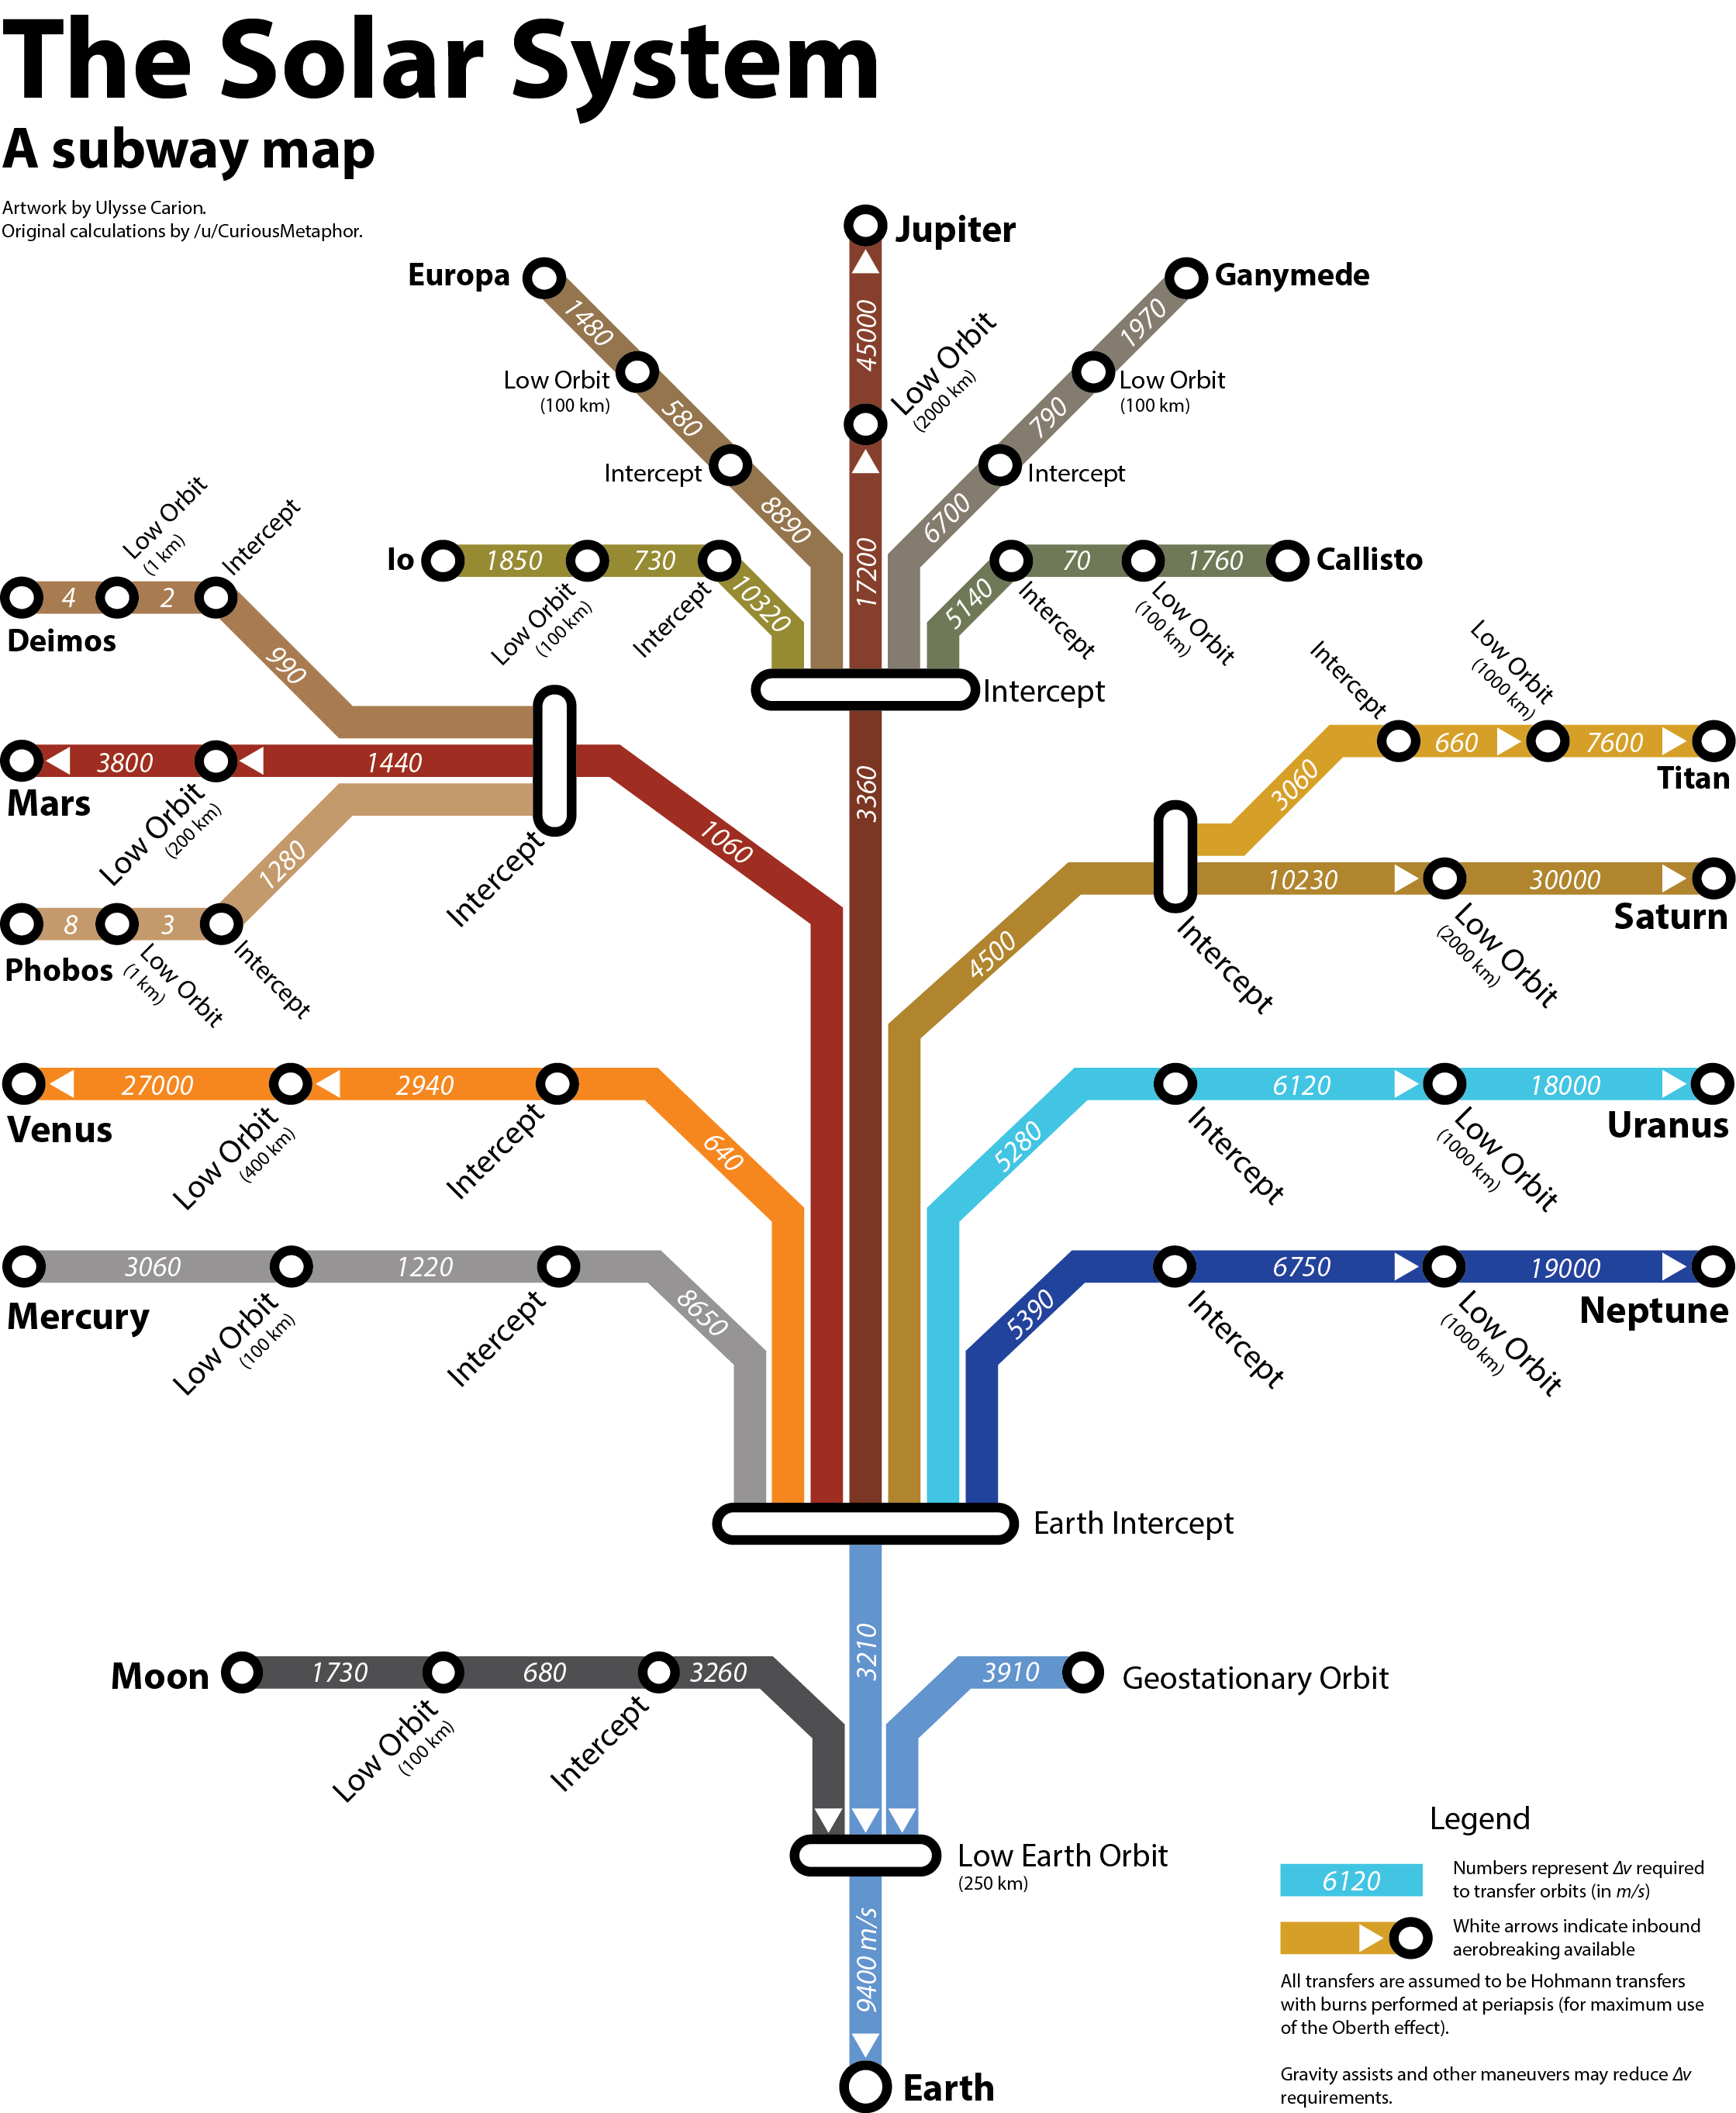
\includegraphics[width=\textwidth]{subway_map}
  \caption{Representation of the different Delta-V needed to go around the solar system, from \citet{reddit-subway}}
  \label{fig-subway_DV}
\end{figure}


For a spacecraft of instantaneous mass $M(t)$, with a propulsion system generating an instantaneous thrust $T(t)$, the Delta-V between $t_1$ and $t_2$ is
\begin{equation} \label{eq-dv}
  \text{Delta-V} = \int_{t_1}^{t_2} \frac{ \norm{T(t)}}{M(t)} dt.
\end{equation}
We see from \cref{eq-dv} that for a more massive spacecraft, a more intense, or a longer thrust is needed in order to obtain the same Delta-V.

\subsection*{Rocket equation}
The thrust $T$ generated by ejecting mass at high velocity is
\begin{equation} \label{eq-thurst}
  T = v_{\rm ex} \dot{M}
\end{equation}
with $v_{\rm ex}$ the exhaust velocity of the propellant, and $\dot{M}$ is the propellant mass flow rate through the thruster.
Hence,
\begin{equation} \label{eq-rocket}
  \text{Delta-V} = \int_{t_1}^{t_2} v_{\rm ex} \frac{ \norm{\dot{M}}}{M(t)} dt = v_{\rm ex} \ln \lp \frac{M_0}{M_1} \rp
\end{equation}
with $M_0 = M(t_0)$ and $M_1=M(t_1)$, and supposing that $v_{\rm ex}$ is constant.
We see from \cref{eq-rocket} that for a given mass $M_1$ to be set to a position after a given Delta-V, the exhaust velocity is a directly link to the initial mass $M_0$.
We usually refer to $M_1$ to the dry mass, and $M_0$ to the wet mass (dry mass plus propellant).
\Cref{eq-rocket} is named the (Tsiolkovsky) rocket equation, 
The exhaust velocity $v_{\rm ex}$ is usually refereed instead by the specific impulse $\Isp = g_0 v_{\rm ex}$, with $g_0$ the standard gravity.
\nomenclature[Q]{\ensuremath{ \Isp}}{ Specific impulse, related to the exhaust velocity of a propellant}
\nomenclature[P]{\ensuremath{ g_0}}{  Standard gravity \nomunit{9.80665 m/s$^2$}}

\subsection*{Chemical and electrical space propulsion systems}
The usual thruster for rocket thruster uses chemical reaction to generate the thrust.
For instance, the Vulcain ( the thruster engine of the main stage of the European Ariane 5 and 6, developed by ArianeGroup, ex Safran) uses the oxygen-hydrogen combustion, the most efficient chemical reaction \citep{nasa-H2O2}
\begin{equation*}
  2 {\rm H_2} + { \rm O_2} = 2 {\rm H_2 O} + 572 \text{~kJ},
\end{equation*}
with the energy of 572~kJ corresponding to 1~mole of oxygen.
This means that burning 1~kg of hydrogen-oxygen mixture deliver an energy of 13~MJ. 

Supposing that of that energy is converted into the exhaust of the water produced, its velocity would be of 5.1~km/s.
In reality, the exhaust velocity of the Vulcain is of 4.2~km/s, corresponding to $\Isp=431$~s.

The fact that the energy source is linked to the propellant mass gives an upper limit of exhaust velocity for a given combustion.
Electrical propulsion engines, on the other hand, decouple the mass ejected (the propellant) from the energy source.
This allows theoretically an unlimited exhaust velocity.
Another advantage is the absence of reactive species, which lowers the security requirements impacting the spacecraft.

\subsection*{Electric propulsion} \label{subsec-label}
\ac{EP} systems mostly rely on plasma \citep{charles2009,mazouffre2016}.
They have been successfully used since the 1960s by governments, but their complexity, the limited electric power available, and the natural risk aversion of the space industry kept the \ac{EP} technologies hidden from the commercial applications \citep{lev2019}.
The breakthrough came in the '90s when the former Soviet Union's companies licenses the technology to western propulsion companies.
However, many commercial satellite manufacturers were sceptical, until the first decade of the 20th century, which brought strong evidences of \ac{EP}.
The landmark of commercial use of \ac{EP} is the selling of 4 all-electric satellites for Geostationary Earth orbit by Boing in 2012, the first 2 of which launched in Marsh 2015.

The two main \ac{EP} technologies used are
\begin{itemize}
  \item the \ac{HET}s, also known as Stationary Plasma Thruster (SPT) in Russia
  \item the Gridded Ion Thrusters (GIT), usually refereed as Ion Thrusters
\end{itemize}

Recently, the first satellites of two mega-constellations (OneWeb, 648 satellites, from which 6 were launched on February, the \nth{26} 2019, and Startlink, 12,000 satellites, from which 62 were launched on May, \nth{23} 2019) were send two Low Earth orbit, both using Hall effect thrusters. 


 
 \paragraph{The Gridded Ion Thruster} is a plasma chamber closed at one end by two or more grids.
 The plasma source is an emitting cathode, generating energetic electrons that ionize the propellant, usually Xenon.
 The ions are accelerated by the potential difference between the grids.
 Another cathode is used to neutralize the ion beam.
 Compared to \ac{HET}s, it produces an ion beam with less divergence and an higher \Isp of the order of 3000 to 4000~s.
 \Cref{fig-iongridded} shows a picture of the ion thruster used for the BepiColombo mission toward Mercury.
 We clearly see the neutralizing cathode, the accelerating grid and the ion beam.
 
\begin{figure}[hbtp]
  \centering
  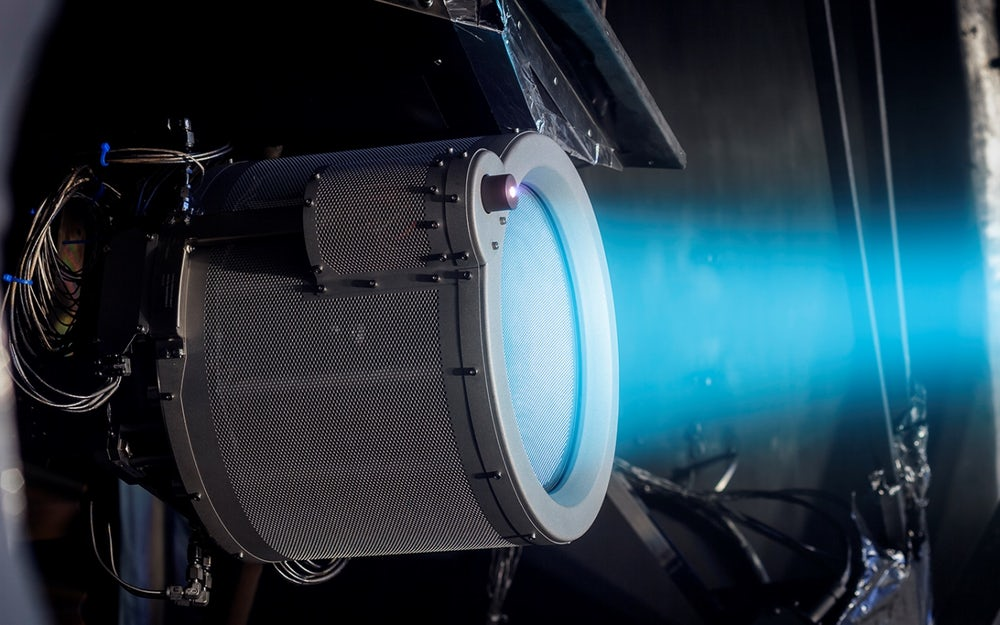
\includegraphics[width=\defaultwidth]{ion_Bepi}
  \caption{The T6 ion thruster will help send BepiColombo to Mercury (Credit: QiniteQ)}
  \label{fig-iongridded}
\end{figure}
 
 \paragraph{Hall Effect thrusters} uses a magnetic barrier to keep the electrons on an annular trajectory, both increasing the ionization of the propellant and creating the accelerating electric field.
 A detailed description of the \ac{HET} is presented in the next section.
 One cathode is used to start the discharge and neutralize the beam.
 Compared to GITs, HETs need less power sources, hence reaching better thrust per power ratio and smaller (hence lighter) Power Processing Unit.
 Their typical \Isp is of the order of 1500~s.
 
 \Cref{fig-13kWHET} shows a high power prototype firing.
 We see the emitting cathode at the center, and the ion beam.
 \begin{figure}[hbtp]
   \centering
   \includegraphics[width=\defaultwidth]{HET_x3}
   \caption{A 13 kilowatt \ac{HET} prototype on a testing bench in a vacuum chamber (Credit: NASA).  }
   \label{fig-13kWHET}
 \end{figure}
 
 
 \subsection*{\ac{EP} environment in France} \label{subsec-HET_thruster}
 
 France is a leader country in the aerospace industry in Europe and in the world, with for example Airbus, Thales, Safran and ArianeGroup.
 Unsurprisingly, its ecosystem of electric propulsion is rich.
 The main French thrusters are the PPS series from Safran, with the \PPS1350 (version G at 1.5~kW nominal power, 89~mN of thrust and \Isp of 1650~s, and the version E at 2.7~kW, at 140~mN of thrust and \Isp of 1800s), and the \PPS5000, a high power \ac{HET} at 5~kW, the first models of which has been delivered to Boeing in May 2019.
 A low-power version of the \PPS{}  is currently developed at Safran \citep{vaudolon2018}.

 
 Several initiative concerning the small-sat sector are also undertaken, as for instance the start-ups Exotrail (micro \ac{HET}) and Thrust Me (radio frequency Ion Thruster), or the Electron Cyclotron Resonance Thruster at ONERA.
 
 A research group on plasma propulsion has been studying \ac{HET} since 1996.
 it is composed of the \ac{CNES}, laboratories as ICARE, LAPLACE and LPP, Safran and ONERA \citep{boniface2017}.
 
 This numerous actors, combined with the support of the France and European space agencies, compose a stimulating environment that contributes both to the most mature technologies and the promising \ac{EP} concepts that could disrupt the propulsion sector.
 
% !TEX root=/home/tavant/these/manuscript/src/manuscript.tex


\section*{\ac{HET} research and development with Safran}
\label{sec-poseidon}
\addcontentsline{toc}{section}{\ac{HET} research and development with Safran}



Safran Aircraft Engines has been collaborating with \ac{LPP} since 2014, starting with the Ph.D. thesis of Viven Croes \citep{croes2017}.
During this first three years, a \ac{2D} \ac{PIC} code has been developed simulating the radial and azimuthal directions of a \ac{HET}.
Azimuthal instabilities have been observed in \citet{croes2017a}, and the effects of alternative propellants have been investigated in \citet{croes2018}.

From this fruitful collaboration, an ANR (Agence National de la Recherche) industrial chair {\sc Poseidon} for  "uture Plasma thrusters for LOw earth orbit SatEllIte propulsiON systems", Grant No. ANR-16-CHIN-0003-01 , has been created.
Its objective is to develop novels methods to reduce the development time and cost of the next \ac{EP} systems.
Both experiments and simulations are being developed to unlock the barriers of \ac{HET} development.
The {\sc Poseidon} chair is linked to the current development of a  low power \ac{HET} at Safran, the \PPS X00, which nominal operating point is of the order of 500W.
The scientific part of the chair is leaded by \ac{LPP}, while an unstructured \ac{3D} simulation code is developed by the CERFACS, in Toulouse.
Safran leads the engineering development and experimental investigation.

At the begining of my thesis, I participated to the development of a \ac{ML} of the \PPS X00.
The objectives of the \PPS X00-\ac{ML}  is to represent the physics of the \PPS X00 while allowing parametric studies of the main parameters of a \ac{HET}, as the geometry, the magnetic field topology, or the wall material.
The \PPS X00-\ac{ML} has successfully showed its usefulness, as the first tests allow to obtain state of the art performances \citep{vaudolon2018}.
My work at Safran showed us that the development of \ac{HET} is still currently driven by experiments, because numerical tools are not yet predictive.
Simulations are helpful for the engineers to have some insights for the thruster behaviour, but cannot be used for development with confidence.
However, experiments are costly and time-consuming.
They also are prone to delays in the conception schedule, and reduce innovation as designers take less risks.

The lack of numerical tools for \ac{HET}  comes from some keys physical phenomena that need to be better understood.


\section*{Key phenomena of \ac{HET}s}
\addcontentsline{toc}{section}{Key phenomena of \ac{HET}s}

Even though \ac{HET} have been studied and used for more than 40 years, some key phenomena are still ill-understood, and then a \emph{trial and errors} method is used for the development by manufacturers.
These key phenomena are
\begin{itemize}
  \item the electron axial transport toward the anode
  \item the plasma-surface interaction 
  \item the wall erosion
  \item the propellant nature
\end{itemize}


\paragraph{The electron axial transport}  through the magnetic barrier has been measured much higher than the expected value from the classical collisional theory by \citet{meezan2001}.
Different phenomena have been proposed to explain the origin of this \emph{anomalous} transport.
Two phenomena are supposed to be mainly responsible for this enhanced mobility\string: the azimuthal instability and the near wall mobility due to electron emission.
A significant part of the work of this Ph.D. thesis concerns the quantitative comparison of the relative importance of the two phenomena.

\paragraph{Plasma-wall interaction} concerns the phenomena that depends of the wall material and affect the discharge.
Indeed, depending on the nature of the wall, the discharge behaviour can vary \citep{gascon2003}.
The phenomenon responsible for this observation is the electron emission, as an electron reaching the wall will have a different probability to emit one or more electrons for different materials.
This affects the particle and power balance of the plasma, hence affecting the sheath and plasma characteristics.
Ion induced electron emission is much less likely to happen as the ions have a small energy of impact.

\paragraph{Wall erosion} is due to sputtering of the ceramic induced by ions impact.
This large erosion is the main limitation of \ac{HET}s lifetime.
While most aspects of the erosion are well understood, we observe the apparition or  patterns with a typical scale of the order of the millimeter in the eroded surfaces that could affect the performances.
The origin, and implication, of these erosion striations stays an open question.

\paragraph{The propellant nature} affects the chemistry of the plasma in the thruster.
Because of its high mass and low ionization energy, xenon has been used since the beginning of \ac{HET}. 
However, it is very costly.
The cheaper, but less effective, propellant of choice is krypton, that started to be used.
Iodine could also be interesting, as it can be stored at room temperature in a solid state.
The impact of the propellant mass and chemistry is not yet clear, and slows down the use of alternative propellants.

\vspace{1em}
The objectives of my thesis, in the context of the {\sc Poseidon} chair focuses on the two first points -- the plasma wall interaction and the electron mobility -- and how they can influence each-other.
\inlinenote{Of the Three point, if I talk about erosions ?}







% !TEX root=/home/tavant/these/manuscript/src/manuscript.tex


\section*{Plasma models and simulations}
\label{sec-simulations}

The plasma is the state of mater were the internal energy is high enough to ionize the atoms.
Depending of the pressure, energy, and time scale, different models are better to describe the plasma.

\paragraph{Boltzmann equation \\}
The Boltzmann equation in \cref{eq-boltzmann} describes the evolution of the particles (atoms, ions and electrons) in the phase space.
The phase space is the set of all possible position $\vect{x}$ and velocity $\vect{v}$.
The evolutions in the phase space are due to forces, diffusion and collisions.

\begin{equation} \label{eq-boltzmann}
\deriv{f}{t}  + \vect{v} \cdot \grad_{\vect{x}} f + \vect{F} \cdot  \grad_{\vect{v}} f = \deriv{f}{t} \at{\rm coll}
\end{equation}
where $f$ is the distribution function of the particle at $\vect{x}, \vect{v}$, and $\deriv{f}{t} \at{\rm coll}$ denotes the effects of the collisions, $\grad$ is the gradient in both the positions (subscript $\vect{x}$) and the velocities (subscript $\vect{v}$)  and $\vect{F}$ is the force applied to the particle.
In the general electro-magnetic case,
\begin{equation*} \label{eq-forceEM}
  \vect{F} =  q \vect{E} + q \vect{v} \times \vect{B}
\end{equation*}
with $q$ the particle charge, $\vect{E}$ the electric field, and $\vect{B}$ the magnetic field.

\paragraph{Fluid equations \\}
The description in 7 dimensions (3 of space, 3 of velocity, and one of time) can complicate the resolution of the Boltzmann equation.
Instead, if the preside description of $f$ is not needed, we can instead use the first moments of \Cref{eq-boltzmann} on the velocity.

The first equation is obtained by integrating \cref{eq-boltzmann} over the velocity space
\begin{align}
  \iiint_{\vect{v}} d^3v \text{ \cref{eq-boltzmann}} &&{ } \iff { }&& \iiint_{\vect{v}}  \deriv{f}{t} d^3v &&+&& \iiint_{\vect{v}}  \vect{v} \cdot \grad_{\vect{x}} f  d^3v &&+&&  \iiint_{\vect{v}}  \vect{F} \cdot  \grad_{\vect{v}} f  d^3v && = && \iiint_{\vect{v}}  \deriv{f}{t} \at{\rm coll} \nonumber  \\ 
  && { } \iff { }&&  \deriv{n}{t} &&+&& \vect{u}  \cdot \grad_{\vect{x}} n &&+&& 0 &&=&& S_{\rm iz}   \label{eq-conc}
\end{align} 
where $n=\iiint f d^3v$ is the density, $\vect{v} = \iiint \vect{v} f d^3v$ is the mean velocity, and $S_{\rm iz}$ is the source term of particle due to ionization.
\Cref{eq-conc} is named the continuity equation.
In the similar fashion, integrating the Boltzmann equation times the velocity of the kinetic energy gives the momentum conservation equation and the energy conservation equation.
This set of equation is simpler to approach, although it relies on more hypotheses.
One of the hypotheses concerns the closure of the system.
Indeed, the continuity equation describes the evolution of the density $n$ but needs the mean velocity $\vect{u}$.
However, the velocity is described by the momentum conservation equation but need the temperature $T$, and so on.

In order to close the system, one has to fix an hypotheses on the higher moment of the distribution function.
A usual closure is the isothermal hypotheses. 
Other closures are the adiabatic hypotheses (no heath flux, the \nth{3} moment of $f$), polytropic law linking the evolution of $n$ with $T$, or the Fourier law for heat diffusion.

\subsection*{Plasma simulation models} \label{subsec-simulations}
As there is two different models to describe the plasma, there is two different simulation methods : the fluid simulations and the kinetic simulations.

The fluid simulations solve the density, mean velocity and temperature of the species, and the electromagnetic fields.
Depending of the conditions, the system of equation can be simplified before resolution.

In electrodynamic conditions, mainly for space plasmas and fusion, the Maxwell equations are coupled to the fluid equations leading to magnetohydrodynamics (MHD).

In the case of electrostatic conditions, has it is usual for cold plasmas, the Poisson equation is coupled to the fluid equations.
Due to the low mass of the electrons compare to the ions, we can suppose the quasi-neutrality of the plasma, leading to the drift-diffusion approximation.

The fluid equations can be solved in \ac{3D}, \ac{2D} or \ac{1D} for space.
In low dimension model, the effects of the missing dimensions is usually added, for instance in the source terms as done by \citet{barral2003a}.

However, some phenomena can only be describes by the shape of the distribution function.
An example of such phenomena is the particle-wave interaction, as the Landau Damping \citep{landau1945,malmberg1964} or the plasma-beam instability \citep{filippychev1990}, for which the gradient of the distribution function in the velocity space is important.
In contrast to the fluid descriptions, \emph{ kinetic} simulations solve for the distribution function for both position  and velocities.
Two approaches are usually used for kinetic simulations:
\begin{itemize}
  \item The Direct-Kinetic (DK) simulations, that discretize \Cref{eq-boltzmann} in the full phase space.
  \item The \ac{PIC}, that uses an ensemble of particles to discretize the distribution function.
\end{itemize} 
While the \ac{DK} simulations use an Eulerian description of the fluid, we can see the \ac{PIC} simulations as a Lagrangian approach.

The \ac{DK} simulations can theoretically better describe the plasma, mostly because there is less numerical noise and we can model binary collision more easily, especially Coulomb collisions.
On the other hand, \ac{PIC} simulations are much more simpler to develop on both a mathematical and a computation perspective.
For instance, the effect of electron emission have been recently studied using \ac{DK} simulation by \citet{cagas2019}, while it has been done since the last century in \ac{PIC} simulations \citep{boswell1988}.




% !TEX root=/home/tavant/these/manuscript/src/manuscript.tex

\section*{Problematic}
\label{sec-problematic}
\addcontentsline{toc}{section}{Problematic}

We have seen in the previous sections that the \ac{HET}s have been studied and used since several decades.
However, several challenges are currently tackled in the \ac{EP} industry, as the most prominent listed by \citet{samukawa2012} \string:
\begin{enumerate}
  \item Performance improvement\string: efficiency, lifetime and cost-effectiveness.
   Lifetime is an important issue and is limited by electrode or wall erosion.
   Lifetime of an electric thruster must be larger than 10 000 h of (reliable) operation.
   \item  Design of more versatile thrusters, i.e. able to operate at different combinations of thrust/propellant velocity.
   \item  Extension of domain of operation to lower power ($\mu$N to 10 mN thrust range) for microsatellites or very precise attitude control.
   \item  Extension to higher power for orbit raising of telecommunication satellites (several tens of kW) and    interplanetary missions (100 kW and more).
   \item Extension of EP to low-altitude spacecraft\string: there is an increasing interest in civil and military spacecraft flying  at altitudes around 100 km where the drag is significant and must be constantly compensated.
\end{enumerate}

The \ac{HET} technology has the potential to answer many of these challenges.
for instance, the lifetime is approached with wall-less and magnetically fielded configuration.
Versatility is tackled with dual-mode \ac{HET} configuration \citep{boniface2017}, low power thruster is attained with $\mu$-thursters \citep{lascombes2018}, and so forth.

Unfortunately, the developed of \ac{HET}s remains principally empirical. 
Two physical phenomena are still unclear, and block the understanding of \ac{HET}s \citep{samukawa2012,adamovich2017}\string:
\begin{itemize}
  \item the electron transport,
  \item the plasma-wall interaction.
\end{itemize}

In parallel to sophisticated diagnostics, efforts in the development of kinetic simulations is pursued.
Indeed, the electron transport is affected by instabilities that can only be described by kinetic models \citep{adam2008a,lafleur2016a}.
In addition, the plasma-wall interaction is also affected by kinetic effects, both concerning the electron emission induced by electron impact \citep{barral2003a,raitses2011,sydorenko2006} and the wall erosion by ion impact sputtering.

Relatively few simulation codes highly parallelized have been developed, that could allow parametric studies.
But the ever increasing computational power available allows bigger simulations to be conducted, with for instance \ac{3D} simulation recently performed \citep{fubiani2018,taccogna2012}, even if a scaling still was needed to obtain the results under a reasonable time.

The objective of the work performed during this thesis was to better understand the inner physics of the \ac{HET} discharge, more precisely the electron transport and the plasma-wall interaction. 
In order to answer this question, a kinetic simulation code, highly parallelized, is developed and used, and order to pin-down the main mechanisms, and propose macroscopic model by the mean of parametric studies.

\vspace{1em}
In Chapter 1, we introduce the simulation model.
Chapter 2 presents the results of a parametric study investigating the wall effect PIC.
In chapter 3, we revisit the sheath model in order to explain the simulation results.
The content of Chapter 4 and 5 are not yet fixed.



% \acresetall

\renewcommand\thechapter\oldthechapter
\renewcommand\chaptername\oldthechaptername

% !TEX root=/home/tavant/these/manuscript/src/manuscript.tex

\chapter{Particle-In-Cell simulations of HETs}
\label{ch-1}
Structure :

{\bf Particle in Cell simulations} 20 pages
\begin{zzz}
  
  1.1 The HET
  1.2 Elements of the 2D PIC-MCC simulations

  1.3 Numerical implementation

  1.4 R-theta simulation: hypotheses
  
  1.5 focus on  Dielectrics : Poisson equation 

  1.6 Axial convection model
  
  1.7 Conclusion
\end{zzz}
\inlinenote{Is missing a part of the HET physics. Like the Boeuf Tutorial. }

The \ac{HET} has been studied since its first designs int he 1960's.
However, the physical processes the govern its behaviour stay ill-understood.
For most of them, as the electron cross field mobility or the plasma-surface interactions, kinetic informations are needed.


The next section present the basics of the \ac{PIC} - \ac{MCC} simulations, and the simulations code \LPPic that is develop at \ac{LPP}.


\inlinenote{add SEE models, discussions concerning the choice we did, a.s.o.}
 
% !TEX root=/home/tavant/these/manuscript/src/manuscript.tex


\subsection{The Hall effect Thruster }
\label{sec-HET}

The \ac{HET} is an electrostatic electrical propulsion system accelerating ions by the mean of an imposed voltage difference.
\Cref{fig-bhtonoff} shows a picture of an \ac{HET} switch on and off.
We can clearly see the plasma in the annular chamber.


\begin{figure}[hbtp]
  \centering
  \includegraphics[width=\defaultwidth]{PPS-ON_OFF.jpg}
  \caption{Front view off an \ac{HET}, the BHT-1500 from Busek, USA}
  \label{fig-bhtonoff}
\end{figure}

We can summarize the composition of an \ac{HET} with four parts:
\begin{enumerate}
  \item The annular chamber.
  \item The injecting anode
  \item The cathode
  \item The magnetic circuit
\end{enumerate}

\begin{figure}[hbtp]
  \centering
  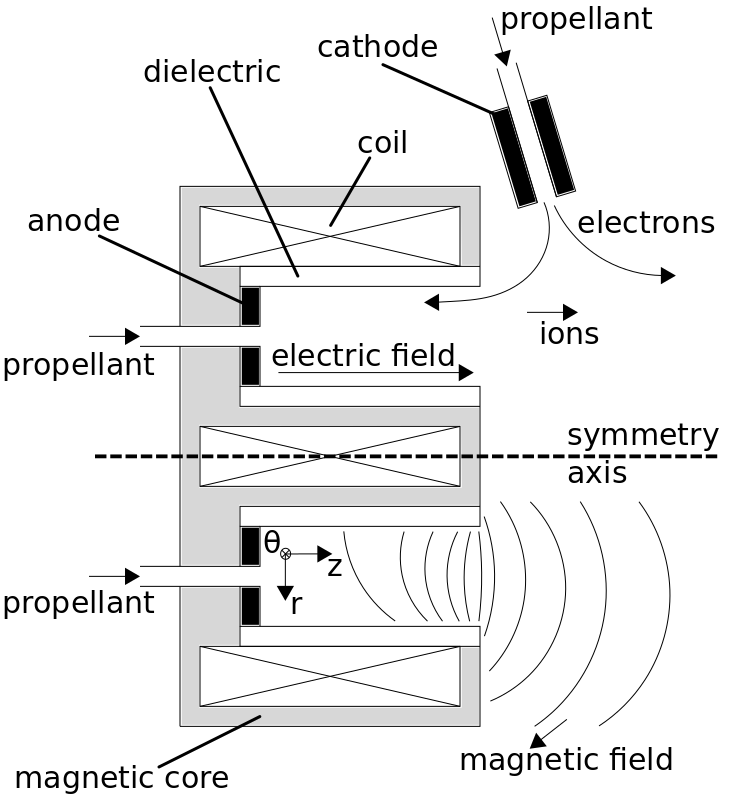
\includegraphics[width=\defaultwidth]{shematic_HET}
  \caption{Schematic cut of an \ac{HET}, illustrating its different parts. }
  \label{fig-shematiccut}
\end{figure}

\Cref{fig-shematiccut} presents a schematic cut of the \ac{HET} along its axial and radial direction.

\paragraph{The chamber} has an annular shape.
It is open closed at the anode side, and kept open at the other side.
The walls are usually constituted by a ceramic, usually \ac{BNSiO2}.
The material needs to be resistant to erosion by ion impact sputtering.
But changing the material is also known to affects the discharge behaviour.
The usually supposed phenomena for this impact is the secondary electron emission yield that is a function of the material nature.


\paragraph{The anode} is at the bottom of the chamber.
The anode voltage is imposed to a few hundred volts.
Usually, the neutral gas injection is made by the anode itself for
The mass flow rate is of the order of a flew mg/s.

\paragraph{The cathode} is outside of the chamber.
It is grounded, and injects electrons for two reasons:
\begin{itemize}
  \item most of the electrons ($\sim 90 \%$) are used to neutralize the ion flux, for both allowing the ions to leave the thruster and avoid charging of the spacecraft.
  \item some of the electrons are attracted by the anode, hence entering the chamber and allowing the plasma discharge and switch and remain on.
\end{itemize}

\paragraph{The magnetic circuit} is composed of electromagnets and a magnetic circuit mode of ferromagnetic material.
It create a constant radial magnetic field in the annular chamber.
The maximum value of the radial magnetic field is located close to the exit plan of the chamber.
Its amplitude is on the order of $200$ Gauss ($\sn{2}{-2}$ T).

\Cref{fig-bshape} illustrate the axial profile of the amplitude of the radial magnetic field.
\begin{figure}[hbtp]
  \centering
  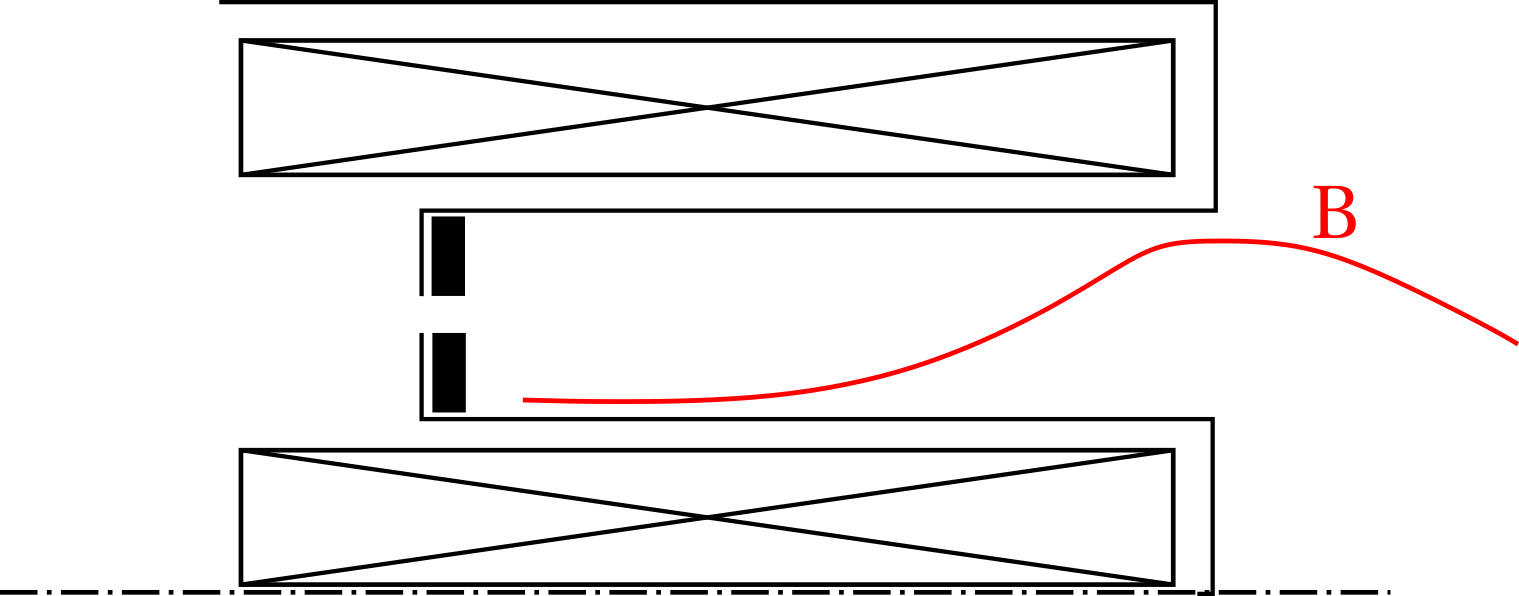
\includegraphics[width=\defaultwidth]{bshape}
  \caption{Usual shape of the axial profile of the radial magnetic field on the centreline of the channel.}
  \label{fig-bshape}
\end{figure}


\subsection{Operating principle}

The operation principle of an \ac{HET} is rather simple.
The objective is to ionize the propellant and impose an electric field to accelerate the ions.

\paragraph{Ionization}
Due to the low pressure (around $\sn{1}{-4}$ Pa), the mean free path of the electrons is too large, compared to the chamber size.
In consequence, we impose the magnetic field in order to trap the electrons in a cyclotron motion, increasing the residence time of the electron, and the ionization.
In average, 90\% of the propellant is ionized in an well designed \ac{HET}.

\paragraph{Acceleration}
The potential difference  between the anode and the cathode is used to accelerate the ions outside of the chamber and create the thrust.
Because the magnetic field slows the electrons down, the plasma resistivity increases in the region where the magnetic field amplitude is large.
Hence, the axial profile of the amplitude of the axial electric field presents a maximum close to the maximum of the magnetic field.

\paragraph{Ionization and Acceleration regions overlay}
As both the ionization region and the acceleration region are governed by the magnetic field, it can be difficult to obtain a net separation.
However, if ionization append in the acceleration region, the newly created ions will not be accelerated at their maximum velocity, hence resulting in a loss compared to the maximum theoretical thrust.

\Cref{fig-zones} shows an illustration of the amplitude of the ionization and the acceleration due tot he electric field.
\begin{figure}[hbtp]
  \centering
  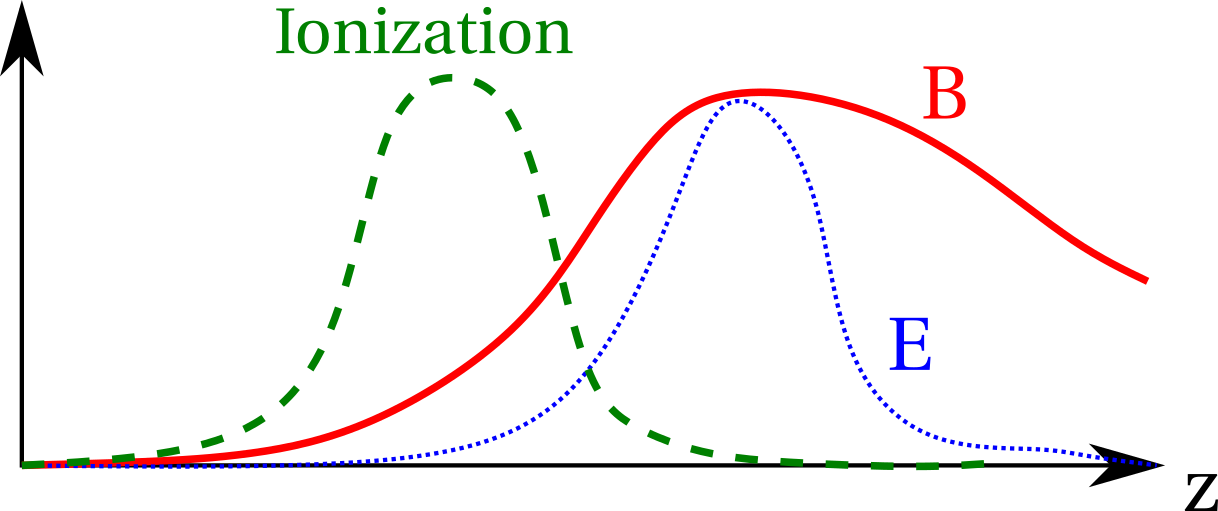
\includegraphics[width=\defaultwidth]{zones}
  \caption{Illustration of the usual axial profiles of the ionization and acceleration amplitude compared to the magnetic field.}
  \label{fig-zones}
\end{figure}

The thruster efficiency, in the usual configuration, is governed by its magnetic field topology.
Hence, it can be difficult to find the best topology that will optimize the ionization and the location of the regions.

Some concepts of double stage \ac{HET} have been proposed to decouple the two phenomena in order to control them independently.
However, the preliminary results are not as satisfactory as expected.
Moreover, the double-stage system needs more parts and power sources, resulting in a more complicated system.
Hence, we keep studying the usual single-stage configuration.

\subsection{Electron Drift and azimuthal instability}
The axial electric field $E$ and the radial magnetic field $B$ induces an azimuthal $E\times B$ drift of the electrons.
Because the ions are not significantly affected by the magnetic field, they do not drift.

As a consequence, they is a strong drift of the electron in respect  to the ions.
This drift can lead to instability in the azimuthal directions.
Because the drift is perpendicular to the magnetic field, it is usually called \ac{ECDI}.
However, as it rises from an $E\times B$ drift, some authors uses the name \ac{EDI}.

Azimuthal oscillations have been observed both experimentally and in simulations.
However, as the \ac{ECDI} characteristic are very close to usual \ac{IAW}, the community is still arguing about the actual kind of wave observed.


\subsection{Plasma-wall interaction}
The ceramic wall closes the chamber in the radial directions.
As usually observed in bounded plasmas, a floating plasmas sheath forms between the plasma and the dielectric wall.
The sheath confines the electrons in the plasma and accelerates the ions toward the walls.
This allows to obtain a flux of electron equals to the flux of ion, resulting in a charge conservation in the plasma, and a neutral flux, also named zero-net current to the surfaces.

Due to the relatively high electron energy, the material can emit electrons induced by electron impact.
These secondary electrons are accelerated toward the plasma, and so modify the plasma and the sheath properties.
The probability of \ac{SEE} depends of the electron impact characteristics (energy, angle) but also of the material: some material are more emitting than others.


\subsection{Cross field transport of the elections}
The electrons are not only drifting in the azimuthal directions.
For instance, because of collisions, the electrons can move from one magnetic line to another.
This leads to a cross-field transport in the direction of the electric field.

It has been observed in \ac{HET} that the electron cross-field transport is higher than the one only due to collisions.
Recently, the \ac{ECDI} has been proposed to induce this so-called anomalous transport of the electrons.

Another phenomena that can leads to increased cross-field transport in the \ac{NWC}.
It is due to electron collisions with the wall, inducing \ac{SEE}.


\section{Three-dimensional physics}
\label{sec-3Dphi}

The physics of the \ac{HET} is really three dimensional:

\begin{itemize}
  \item The plasma is accelerated in the axial direction. The axial profile of the magnetic field is responsible for the performance of the thruster.
  \item The radial dimension is closed by the chamber walls. The walls are responsible for most of the plasma losses, both on the particle and energy balances.
  \item The electrons drifts in the azimuthal direction, leading to instabilities.
\end{itemize}

Consequently, when simulating an \ac{HET}, if one of the direction is not model, a part of the physics will be missing:
\begin{itemize}
  \item Missing axial direction: the ionization and the convection are missing
  \item Missing radial direction: the wall losses and interactions are missing
  \item Missing azimuthal direction: the \ac{ECDI} is missing, hence the electron cross-field transport is not well represented.
\end{itemize}

While 3D-simulations have recently been proposed, they uses scaling laws to simulate the system in a reasonable amount of time.
A simulation at scale {1:1} is not yet accessible.
Hence, we need to rely on \ac{1D} or \ac{2D} simulations.
Consequently, we need to take into account the missing physics or include a model of its effects on the system.

% !TEX root=/home/tavant/these/manuscript/src/manuscript.tex

\section{Elements of the 2D PIC-MCC simulations}
  \label{sec-elements}
  \subsection{Principe of the PIC simulations}

    The \ac{PIC} simulation models particles moving freely on a grid.
    The grid is used to compute the electric field, in the electrostatic approximation by solving the Poisson equation

    \begin{equation}
      \label{eq-poisson}
      \Delta \phi = - \frac{\rho}{\epsilon_0}
    \end{equation}

    where $\phi$ is the electric potential, $\rho$ is the charge density, and $\epsilon_0$ the vacuum permittivity.
    If the electrostatic approximation is not correct, one needs to solve the Maxwell equations.

    The particles move following the Lorenz forces
    \begin{equation}
      \label{eq-Lor}
      m \vec{a} = q \vect{E} + q \vec{v} \times \vec{B}
    \end{equation}
    with $m$ and $q$, the particle mass and electric charge, respectively.
    The numerical particles followed in the simulations correspond to $q_f$ physical particles, with
    \begin{equation}
      q_f = \frac{n V}{\Npc}
    \end{equation}
    with $n$ the particle density, $V$ the volume of a cell, and $\Npc$ the number of numerical particles in a cell.
    A large enough number of particles is needed in order to obtain physical results.
    Indeed, an insufficient number of particles leads to numerical heating \cite{ueda1994}.
    Usually, a minimum of 100 particles per cell are used, but recent results seem to encourage to use more particles \cite{janhunen2018}.

  \subsection{Monte Carlo collisions}

    In \ac{PIC} simulations, collisions between charged and neutral particles can be modeled by binary collision, but this approach is computationally costly.
    Instead, a Monte-Carlo algorithm can be used \cite{vahedi1995}.
    This approach is very efficient and allows scattering, momentum transfer, and ionization to be consistently modeled.
    The propellant used in \ac{HET} is \ac{Xe}.
    The cross-sections used for modeling \ac{Xe} or other gases collisions are taken from the {\sc LXCat} database project \cite{LXCat_web,pancheshnyi2012}.
    Except if otherwise stated, the elastic, inelastic scattering and ionization reactions listed in \cref{tab-reactXe} are used.
    The cross-section values are summarised in \cref{fig-xexsection}.

    \begin{table}[hbtp]
      \ra{1.3}
      \centering
      \caption{Reactions for xenon used in the PIC simulations}
      \label{tab-reactXe}
      \begin{tabular}{@{}lll@{}}  \toprule
        Reaction & Threshold & Reference\\ \midrule
        {\it Elastic scattering} & &\\
        e + Xe = e + Xe   & --   & \cite{Lxcat_Xe,Lxcat_Xe2} \\
        {\it Excitation} & &\\
        e + Xe = e + Xe$^*$   & 8.315eV   & \cite{Lxcat_Xe,Lxcat_Xe2} \\
        e + Xe = e + Xe$^*$   & 9.447eV   & \cite{Lxcat_Xe,Lxcat_Xe2} \\
        e + Xe = e + Xe$^*$   & 9.917eV   & \cite{Lxcat_Xe,Lxcat_Xe2} \\
        e + Xe = e + Xe$^*$   & 11.7eV    & \cite{Lxcat_Xe,Lxcat_Xe2} \\
        {\it Ionization} & &\\
        e + Xe = e + Xe$^+$   & 12.13eV   & \cite{Lxcat_Xe,Lxcat_Xe2} \\
        \bottomrule
      \end{tabular}
    \end{table}



    \begin{figure}[hbtp]
      \centering
      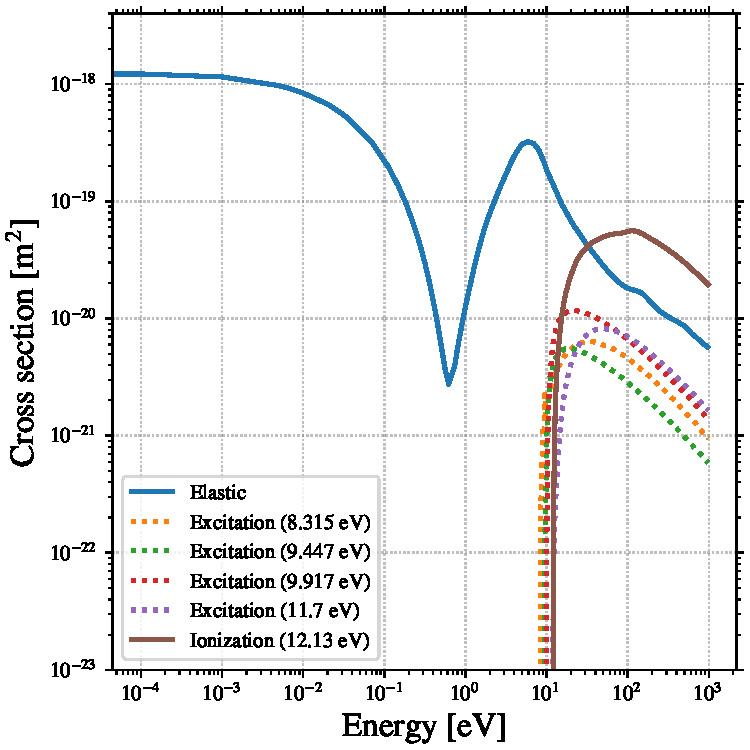
\includegraphics[width=\defaultwidth]{figure/xenon_cross_section.pdf}
      \caption{Cross section values used in the Monte Carlo procedure \cite{Lxcat_Xe,Lxcat_Xe2}.}
      \label{fig-xexsection}
    \end{figure}


\section{Numerical implementation of the Particle in cell simulation}

  \LPPic is an explicit electrostatic \ac{PIC}-\ac{MCC} simulation code.
  Every time-step, the simulation loop presented in \cref{fig-picloop} is computed.
  The different steps constituting the PIC-loop are described in the next subsections.
  \begin{figure}[hbtp]
    \centering
    \smartdiagramset{circular distance=4.5cm,
    module minimum width=3.5cm,
    text width=3cm,
    arrow tip=to}
    \smartdiagram[circular diagram:clockwise]{Particle Motion ,Boundary,Collision,Density weighting, Poisson Equation, Field weighting}
    \caption{\ac{PIC}-\ac{MCC} loop executed every time step.}
    \label{fig-picloop}
  \end{figure}


  \subsection{Data used}
    In \ac{PIC} simulations, there are two kinds of data used\string:
    \begin{itemize}
      \item Particles (electrons, ions, neutrals can be followed as well but not in \LPPic)
      \item Mesh, also named fields (densities, electric and magnetic fields, and so on)
    \end{itemize}

    \paragraph{Particles\\}
    For each particle, are known its position $\vec{x}$ and its velocity $\vec{v}$.
    In most \ac{PIC}-\ac{MCC} simulations, the three directions of the velocity vector are followed in order to take into account scattering.
    It is abbreviated as \acs{3V}.
    The particle positions and velocity are not discretized, except to the numerical floating-point precision.

    \paragraph{Fields\\}
    The fields are defined at the center of each cell of the mesh.
    The charge density $\rho$ is computed by depositing the particle on the mesh, using the Cloud-in-cell model \cite{birdsall1991}.
    The electric field at the position of the particle is also obtained by bilinear interpolation.
    The mesh dimension defines the dimension of the simulation.
    It is usual to find \acs{1D}\acs{3V} or \acs{2D}\acs{3V} \ac{PIC} simulations, for particles with 3 directions on the velocity but one (or two) dimensions in space.

    \subsection{Particle pusher}
    The interaction of the movement equation \cref{eq-Lor} is different for magnetized and non-magnetized particles.
    For non-magnetized particles, we use the leapfrog scheme \cite{birdsall1991}
    \begin{align}\label{eq-leapfrog}
      \vect{v}^t &= \vect{v}^{t-1} + \frac{q}{m} \vect{E} \dt, \\
      \vect{x}^t &= \vect{x}^{t-1} + \vect{v}^t \dt,
    \end{align}
    with the superscript $t$ designing the time step, $q$ and $m$ the particle electric charge and mass, $\vect{E}$ the electric field at the particle position, and \dt the time step duration.

    It is important to note that the leapfrog induces a shift of $\frac{\dt}{2}$ between the position and the velocity, as illustrated in \cref{fig-leapfrog}.
    \begin{figure}[hbtp]
      \centering
      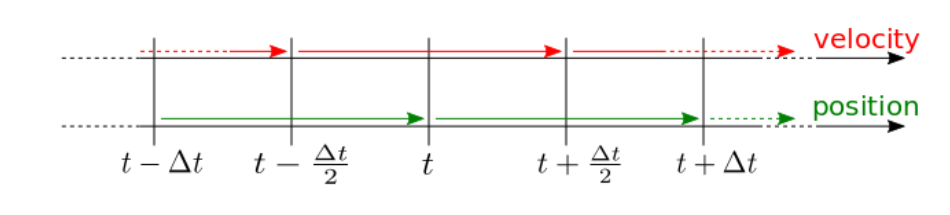
\includegraphics[width=\defaultwidth]{leapfrog.png}
      \caption{Illustration of the shift between the particle velocity and position.}
      \label{fig-leapfrog}
    \end{figure}
    This shift can lead to erroneous diagnostics when computing moments of the particles distribution.
    For instance, the mean velocity of an ensemble of $N$ particles at the instant $t$ is computed as\string:
    \begin{equation} \label{eq-meanv}
      \mean{\vect{v}}^t = \frac{1}{N} \sum_i^N \lp \vect{v_i}^t + \frac{q}{m} \vect{E_i} \frac{\dt}{2} \rp.
    \end{equation}
    Other moments like the mean energy or heat flux follow the same correction.
    We can see that the error between $\mean{\vect{v}}$ defined above and
    $$ \tilde{\vect{v}} = \frac{1}{N} \sum_i^N  \vect{v_i}^t $$
    is
    $$ \mean{\vect{v}} - \tilde{\vect{v}} =\frac{q \dt}{2 m}  \frac{1}{N}  \sum_i^N  \vect{E_i} .$$
    Hence, the error in the diagnostic is larger in the region of large electric field (as in the sheaths).

    \paragraph{Magnetized particles}
    For magnetized particles, we use a modification of the leapfrog algorithm proposed by Boris \cite{boris1970}.
    It corresponds to an operator splitting between the electrostatic acceleration and the magnetic rotation.
    This splitting is described below\string:

    \begin{enumerate}
      \item accelerate the particle during $\frac{\dt}{2}$\string: $\vect{v}^{t-\frac{\dt}{2}} = \vect{v}^{t-1} + \frac{q}{m} \vect{E} \frac{\dt}{2}$
      \item rotate the particle velocity with the magnetic field
      \item accelerate the particle during $\frac{\dt}{2}$\string: $\vect{v}^t = \vect{v}^{t-\frac{\dt}{2}} + \frac{q}{m} \vect{E} \frac{\dt}{2}$
    \end{enumerate}


  \subsection{Poisson equation solver}
  \label{subsec-poissonintro}

    In order to compute the electric field due to the particle charge density, the Poisson equation \cref{eq-poisson}  needs to be discretized over the mesh.
    We can directly discretize the differential operator by using the finite volume approach over a cell of the mesh.
    The formal discretization is developed in \cref{sec-diel}, for the particular case of taking into account the presence of dielectric boundaries.

    In \ac{1D}, the obtained linear system is tridiagonal.
    It can be solved directly using {\sc Thomas}' algorithm, which stores the Gauss elimination's coefficient.
    In \ac{2D}, the linear system is pentadiagonal.
    A direct solver, like the $LU$ decomposition, would require a large amount of memory to store the factorization matrices.
    On the other hand, as the time step is usually small in \ac{PIC} simulation, we expect the plasma potential $\phi$ not to change rapidly.
    Hence, an iterative solver using the previous solution as an initial guess seems more reasonable from both the memory storage and the computational time.
    
    \inlinenote{Anne: dire ici dans quelle section, tu vas en reparler}
    

    
% !TEX root=/home/tavant/these/manuscript/src/manuscript.tex

\section{Bidimentionnal simulation of an \ac{HET}}

We are interested in studying the azimuthal instabilities and the induced electron transport in the axial direction.
In addition, we want to study the plasma-wall interactions.
As realistic \ac{3D} simulations are not yet achievable, we choose to simulate the radial-azimuthal plan.
The axial location where the electron drift is the highest is close to the exit plan, where the axial electric field is the highest.
Hence, we choose this location to be simulated.
In this section, we describe the characteristics of the radial-azimuthal simulation.


\subsection{Neglecting curvature}
The \ac{ECDI} features oscillations of short wavelength of the order of the mm.
Hence, neglecting the curvature of the channel is expected not the change the \ac{ECDI} characteristics while improving the simulation performances.

In  \citet{heron2013},  the authors have performed a \ac{2D} \ac{PIC} simulation including the channel curvature.
They have observed a small difference between the inner and the outer walls.
In  \citet{dominguez-vazquez2018}, the authors studied the effect of the curvature using a \ac{1D} radial model.
They have shown asymmetries due to the combination of the geometric expansion, the magnetic mirror effect, and the centrifugal force.
However, the global behavior of the discharge is not affected compared to simulations without the curvature model.
Hence, in order to simplify the analogy, we choose to neglect the curvature.

Consequently, we can use a Cartesian mesh (also called a rectangular mesh).
The usual notation $x,y$ is used in the simulation for the radial ($r$) and azimuthal directions $\theta$, respectively.
The $z$ component corresponds to the axial direction, normal to the simulation domain.

\subsection{Radial-azimuthal domain description}

The azimuthal direction is closed using a periodic boundary condition for both the particles and the fields.
The radial direction is closed by walls.
The walls can be grounded metallic, or a dielectric boundary can be model.
They are described and discussed in \cref{sec-diel}.

A constant and uniform magnetic field $B_0$ is imposed in the radial direction.
This does not take into account the magnetic mirror, that has been shown to be important \citep{keidar2005,yu2008a,dominguez-vazquez2018}.
However, it cannot be modeled in the \ac{2D} Cartesian radial-azimuthal domain while conserving a divergent-free magnetic field topology.
A constant and uniform axial electric field $E_0$ is imposed.
\Cref{fig-2dschemat} shows a schematic representation of the simulated domain, overlaid with the computed azimuthal electric field $E_y$.

\begin{figure}[hbtp]
  \centering
  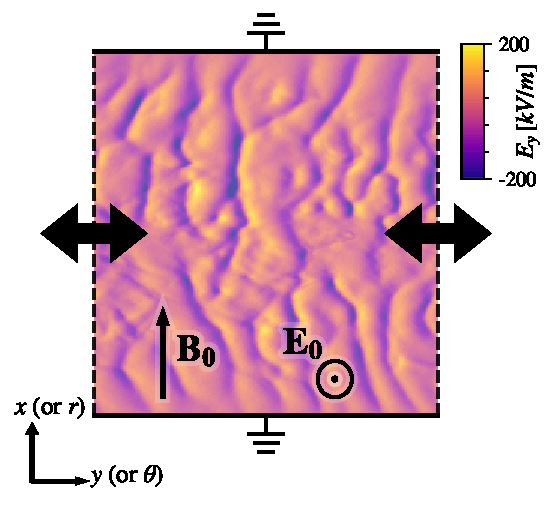
\includegraphics[width=\defaultwidth]{2D_schema.pdf}
  \caption{Schematic representation of the radial-azimuthal simulation domain. Overlaid is the computed azimuthal electric field given as an example. The radial dimensions lengths 2\,cm, and the azimuthal length is 1\,cm.
  The magnetic field is $B_0=0.02\,\tesla$, the axial electric field is $E_0=\sn{2}{4}\,\volt\per\meter$, and the walls are grounded. More parameters are given in \cref{parameters}.}
  \label{fig-2dschemat}
\end{figure}

\subsection{Particle balance}
As the axial position simulated is the exit plane, the ionization is too low to balance the particle losses to the wall.
Instead, the ionization takes place upstream, and the particles are convected downstream.
In these conditions, two models can be used concerning the particle losses at the walls\string:
\begin{itemize}
  \item having a simulation that dies off, as done in \citet{janhunen2018},
  \item forcing an arbitrary ionization to occur in order to compensate the radial losses \citep{dominguez-vazquez2018}.
\end{itemize}
The second option is slightly less realistic, but allows to obtain a steady-state and is supposed not to affect the simulation significantly.
Hence, we use this model to achieve a constant mean plasma density during the simulation.
The forced ionization rate is computed in order to compensate the losses of the ions at each time step.
The spacial ionization  profile is uniform.


\subsection{Axial convection}

Due to the imposed axial electric field, ions and electrons gain energy.
In the \ac{HET}, the axial convection of the particles balances the energy gain.
However, in a purely \ac{2D} simulations, the convection is missing, resulting in an ever-rising particle energy.
This prevents the possibility to reach a steady-state regime, as observed in \citet{heron2013,janhunen2018}.

We implemented a model of convection initially proposed for a \ac{1D} simulation by \citet{lafleur2016a}, and adapted in \ac{2D} by \citet{croes2017a}.
The model uses a finite axial length $L_z$.
When a particle reaches the boundary $z=0$ or $z=L_z$, it is removed from the simulation.
In order to conserve the particle (and charge) balance, a particle is created at $z=0$ for the ions (that are accelerated toward $z>0$) or at $z=L_z$ for the electrons.
It has been observed that using a radial position chosen uniformly at random for the newly injected particle would affect the sheath \citep{croes2017a}.
Hence, the radial position of the new particle is the same as the removed particle.

Concerning the azimuthal particle position, it is more difficult to choose between a random position or the same position as the removed particle.
In \citet{lafleur2016a,croes2017a}, a random azimuthal position was chosen.
However, as will be discussed in \cref{sec-reinjectionnoise}, this induces a numerical noise that can be harmful in some cases.

% !TEX root=/home/tavant/these/manuscript/src/manuscript.tex

\section{Dielectrics boundary condition}
  \label{sec-diel}

  \Cref{fig-2dschemat} shows the simulation of the radial-azimuthal domain with metallic grounded walls.
  \Cref{fig-2D} illustrates the configuration in the radial-azimuthal plane highlighting the more realistic radial boundary conditions.
  The plasma is bounded in the radial direction by dielectric layers isolating the magnetic circuit.
  The magnetic circuit can be considered electrically grounded.

  The particles are absorbed when touching the dielectric wall, and we suppose an infinite residence time.
  Hence, we obtain a surface charge $\sigma$ at a time $t$ with
  \begin{equation} \label{eq-sigmaintegrate}
    \sigma(t) = e \int_0^t (J_i - J_e) dt
  \end{equation}
  with $J_i$ and $J_e$ the ion and electron flux respectively and $e$ is the elementary charge and supposing that there is no surface charge at the interface at the beginning.

  \begin{figure}[hbt]
    \centering
    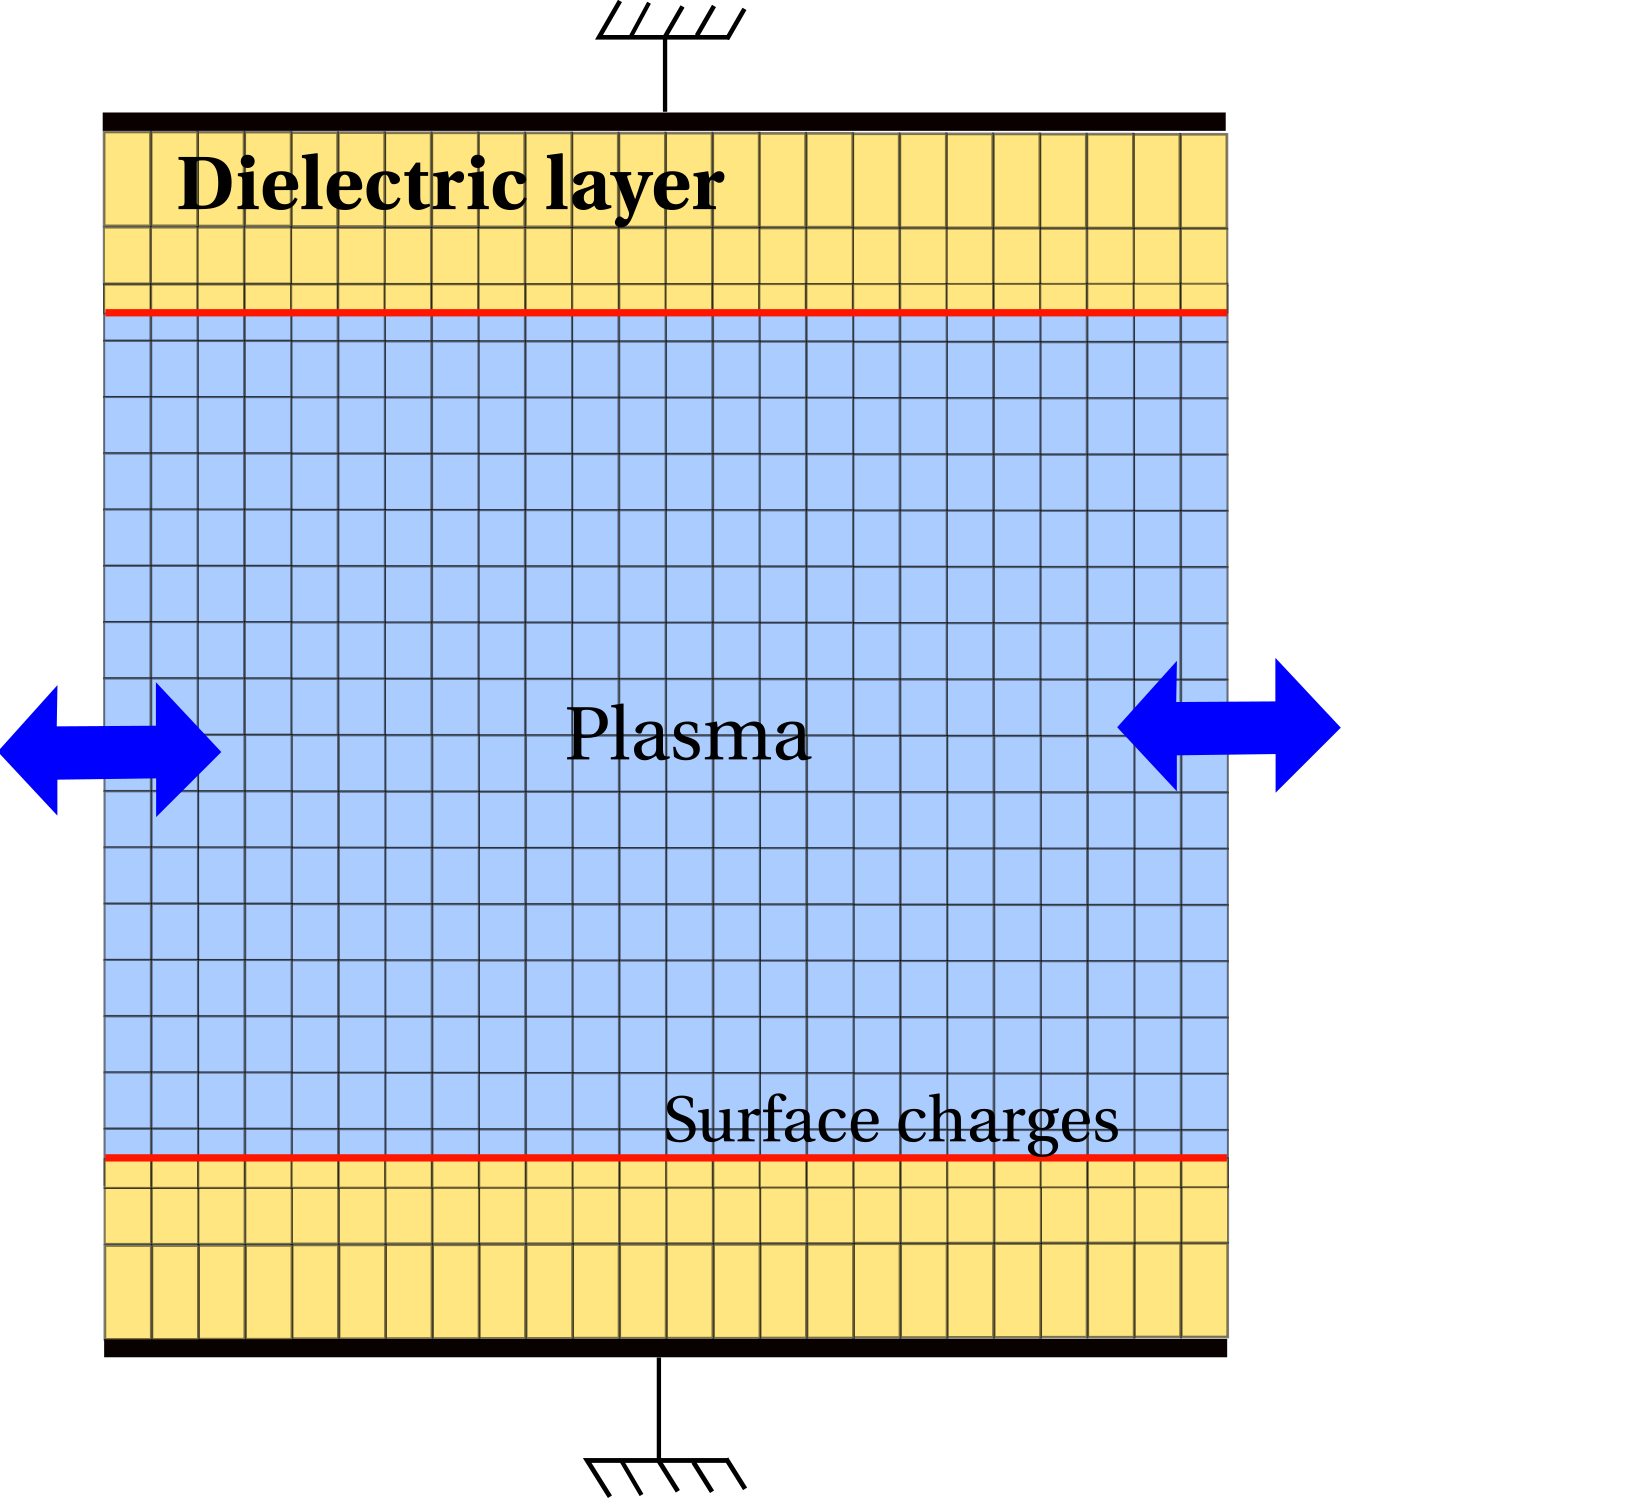
\includegraphics[width=\defaultwidth]{2D_diel_Rtheta}
    \caption{Schematic representation of the dielectric layers between the plasma in the \acs{2D} radial-azimuthal plane. Are present the dielectric in yellow, the plasma in blue, the surface charges in red, and the grounded magnetic circuit in black.}
    \label{fig-2D}
  \end{figure}


  A common approach is to assume that the electric field inside the dielectric is zero \citep{taccogna2019}. 
  Using Gauss theorem, we obtain a Neumann boundary condition at the plasma-wall interface for the potential
  \begin{equation} \label{eq-gauss}
    \norm{\partial_r \phi} = \frac{\norm{\sigma}}{\epsilon_0}
  \end{equation}
  with $\sigma$ the surface charge and $\epsilon_0$ the vacuum permittivity.
  However, the electric field in a dielectric material is not zero but depends on the global system.
  Hence, in order to model the dielectric wall of the \ac{HET} correctly, we choose to include the whole dielectric layers inside of the simulation domain.

  In this section, we derive the discretization of the Poisson equation with a non-uniform permittivity in the \ac{2D} radial azimuthal plane using the finite volume approach.


  \subsection{Non-uniform mesh}

    In the dielectric layers, there is no particle nor charge.
    Hence, the numerical constraints on the cell size are not applicable, and the cell size can be increased.
    In order to reduce the cell size difference between two neighboring cells, we use an exponential growth of the cell size in the radial direction.
    The cell size in the azimuthal direction $\dy$ is kept constant.
    The resulting non-uniform mesh can be seen in \cref{fig-2D}.


  \subsection{Poisson equation discretization}


  The dielectric permittivity is $\epsilon= \epsr \epsilon_0$ with $\epsr$ the relative permittivity of the dielectric.
  The Poisson equation with a not-constant permittivity is
  \begin{equation} \label{eq-poissondiel}
    \grad \cdot \epsilon \grad \phi = \rho
  \end{equation}
  with $\rho$ the charge density.
  We note $\vect{D}=\epsilon \vect{E} = \epsilon \grad \phi$ the electric flux.
  \Cref{fig-decompo1} shows the Cartesian decomposition of the \ac{2D} domain.
  The cell $(i,j)$ has four direct neighbors\string:
  \begin{itemize}
    \item the east $E$ in $(i+1,j)$
    \item the west $W$ in $(i-1, j)$
    \item the north $N$ in $(i, j+1)$
    \item the south $S$ in $(i, j-1)$
  \end{itemize}
  The cell dimensions are $\dx_{i,j}$ and $\dy_{i,j}$, and $\V=\dx_{i,j} \dy_{i,j}$ is the cell volume.
  As the mesh is Cartesian, we have for a given $j$ $\dx_{i,j} = cst$ for all $i$. Hence, we note $\dx_{i,j} = d_i$ and $\dy_{i,j} = d_j$

  The boundaries are noted $S^s_{i,j}$ with $s=E,W,N$ or $S$.
  We can see that $S^W_{i,j}=S^E_{i-1,j}$, and the same goes for the other borders.
  We note $\C = S^E_{i,j} \cup S^W_{i,j} \cup S^N_{i,j} \cup S^S_{i,j}$ the cell surface boundary.
  The center of the cell is located in $i,j$ and the borders are located in $i\pm 1/2$ in the East-West direction and $j\pm 1/2$ in the North-South direction.
  \begin{figure}[hbt]
    \centering
    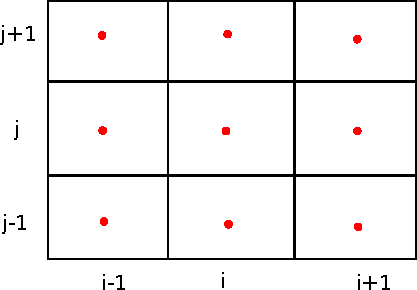
\includegraphics[width=\defaultwidth]{discrect1.pdf}
    \caption{Illustration of the Cartesian decomposition of the \acs{2D} domain}
    \label{fig-decompo1}
  \end{figure}


  \subsection{Poisson equation discretization}

    We start by positioning the plasma-dielectric interface on the surface between two cells.
    This means that the permittivity $\epsilon = \epsilon_0 \epsr$ is  constant over a cell.
    In order to discretize the Poisson equation, we integrate \cref{eq-poissondiel} over the cell volume

    \begin{equation}
    \int_{\V} - \grad \cdot (\epsilon \grad \phi) dv= \int_{\V} \rho dv.
    \end{equation}
    Using Gauss-Ostrogradsky theorem, we obtain
    \begin{equation}
    \oint_{\C} ( - \epsilon \grad \phi) \cdot \vect{n} dS = Q_{tot} =  \V \bar{\rho},
    \end{equation}
    with $\vect{n}$ the normal vector directed outward, $Q_{tot}$ is the total charge of the cell and $\bar{\rho}$ is the mean value of $\rho$ in the cell.
    We can decompose the integration over the cell boundary with the four surfaces $S^s_{i,j}$ as
    \begin{equation}
      \label{eq-poissonsum}
    \oint_{\C} (-\epsilon \grad \phi) \cdot \vect{n} dS = \sum_{k\in(E,W,N,S)} S^k_{i,j} \vect{D}^k_{i,j} \cdot \vect{n}
    \end{equation}
    with $\vect{D}^k_{i,j}$ the flux through the surface $k$ of the cell $(i,j)$.


    \paragraph*{Electric flux \\}
    Let us define the electric flux through the East border  $\vect{D}^E_{i,j}$.
    We suppose there is no surface charges on $S^E$.
    We can hence write the electric flux as
    \begin{align} \label{eq-flux1}
      \vect{D}^E_{i,j} \cdot \vect{n} &= \epsilon_{i,j} E_{x, i+1/2,j}^-\\
                                      &= - \epsilon_{i,j} \frac{\phi_{i+1/2,j} - \phi_{i,j}}{d_i/2},
    \end{align}
    with an off-center discretization of the electric field.
    Using the Gauss's law without charges
    \begin{equation} \label{eq-gausslaw}
      \epsilon_{i,j}E_{x, i+1/2,j}^- - \epsilon_{i+1,j}E_{x, i+1/2,j}^+ =0,
    \end{equation}
    we have
    \begin{equation}
      \epsilon_{i,j} \frac{\phi_{i+1/2,j} - \phi_{i,j}}{d_i/2} = \epsilon_{i+1,j} \frac{\phi_{i+1,j} - \phi_{i+1/2,j}}{d_{i+1}/2}.
    \end{equation}
    Hence
    \begin{equation} \label{eq-phidemi1}
      \phi_{i+1/2,j} = \frac{\epsilon_{i,j} d_{i+1} \phi_{i,j} + \epsilon_{i+1,j} d_{i} \phi_{i+1,j} }{\epsilon_{i,j} d_{i+1} + \epsilon_{i+1,j} d_{i} },
    \end{equation}
    which corresponds to the usual discretization \citep{croes2017} when $\epsilon$ and $d_i$ are both constant.
    Using \cref{eq-phidemi1} in \cref{eq-flux1} we obtain
    \begin{align}
      \label{eq-nosc}
    \vect{D}^E_{i,j} \cdot \vect{n} &=& 2\frac{\epsilon_{i,j}\epsilon_{i+1,j}}{\epsilon_{i,j}d_{i+1} + \epsilon_{i+1,j} d_i} (\phi_{i,j}-\phi_{i+1,j})
    &=& 2\epsilon_0 \frac{\epsr{i,j}\epsr{i+1,j}}{\epsr{i,j}d_{i+1} + \epsr{i+1,j} d_i} (\phi_{i,j}-\phi_{i+1,j})
    \end{align}

    We note $Q^E_{i,j} \equiv \frac{\epsilon_{i,j} \epsilon_{i+1,j}}{\epsilon_{i,j} d_{i+1} + \epsilon_{i+1,j} d_i}$.
    reproducing the same decomposition on the other borders, we obtain
    \begin{equation}
      \label{eq-descretPoisson1}
    S^E_{i,j} Q^E_{i,j} \phi_{i+1,j} + S^W_{i,j} Q^W_{i,j} \phi_{i-1,j} + S^N_{i,j} Q^N_{i,j} \phi_{i,j+1} + S^S_{i,j} Q^S_{i,j} \phi_{i,j-1} - Q^C_{i,j} \phi_{i,j} = - \V \bar{\rho_{i,j}}
    \end{equation}
    with
    \begin{center}
      $\begin{dcases}
     Q^E_{i,j} &= 2\frac{\epsilon_{i,j} \epsilon_{i+1,j}}{\epsilon_{i,j} d_{i+1} + \epsilon_{i+1,j} d_i} \\
     Q^W_{i,j} &= Q^E_{i-1,j} \\
     Q^N_{i,j} &= 2\frac{\epsilon_{i,j} \epsilon_{i,j+1}}{\epsilon_{i,j} d_{j+1} + \epsilon_{i,j+1} d_{j}}\\
     Q^S_{i,j} &= Q^N_{i-1,j} \\
     Q^C_{i,j} &= Q^E_{i,j}S^E_{i,j}+Q^W_{i,j}S^W_{i,j}+Q^N_{i,j}S^N_{i,j}+Q^S_{i,j}S^S_{i,j}
     \end{dcases}$
    \end{center}

    as well as $S^E_{i,j} = S^W_{i,j} =d_id_z, S^N_{i,j} = S^S_{i,j}= d_jd_z$ et $\V = d_jd_id_z$.
    We observe that the evolution of the relative permittivity and the cell size affects the coefficients to be used, but the system remains symmetric as we have $Q^S_{i,j} = Q^N_{i-1,j}$ and $ Q^W_{i,j} = Q^E_{i-1,j}$.
    
    A symmetric system is a linear system of equation $A \cdot X = B$  which matrix $A$ is equal to its transpose\string: $A = A^T$.
    It allows reducing by a factor of two the memory needed to store the matrix.
    It also allows to use algorithms exploiting this aspect.
    For instance, the eigenvalues are real-valued, and the matrix factorization only need to store one factor using Cholesky decomposition, which gives $A = L L^T$ with $L$ a lower-triangular matrix. 

    \subsection{Including surfaces charges}
    Let's now considerer the presence of surface charges on the surface $S^E_{i,j}$.
    Gauss's law now reads
    \begin{equation} \label{eq-gausslawsc}
      -\epsilon_{i,j}E_{x, i+1/2,j}^- + \epsilon_{i+1,j}E_{x, i+1/2,j}^+ =\sigma^E,
    \end{equation}
    with $\sigma^E$ the surface charge on the surface.
    The surface charge is not taken into account when computing the total charge in a cell.
    Using the same discretization as before, we obtain
    \begin{equation}
    \epsilon_{i,j} \frac{\phi_{i+1/2,j} - \phi_{i,j}}{d_i/2} - \epsilon_{i+1,j} \frac{\phi_{i+1,j} - \phi_{i+1/2,j}}{d_{i+1}/2} = \sigma^E
    \end{equation}
    so that
    \begin{equation}
      \label{eq-phidemi}
    \phi_{i+1/2,j} = \frac{\epsilon_{i,j} d_{i+1} \phi_{i,j} + \epsilon_{i+1,j} d_{i} \phi_{i+1,j} }{\epsilon_{i,j} d_{i+1} + \epsilon_{i+1,j} d_{i} } + \frac{1}{2}\sigma^E \frac{d_i d_{i+1}}{\epsilon_{i,j} d_{i+1} + \epsilon_{i+1,j} d_{i}}
    \end{equation}
    hence
    \begin{align*}
    \vect{D}^E_{i,j} \cdot \vect{n} &= 2\frac{\epsilon_{i,j}\epsilon_{i+1,j}}{\epsilon_{i,j}d_{i+1} + \epsilon_{i+1,j} d_i} (\phi_{i,j}-\phi_{i+1,j}) - \sigma^E \frac{\epsilon_{i,j}d_{i+1}}{\epsilon_{i,j}d_{i+1}+\epsilon_{i+1,j}d_{i}}
    \end{align*}
    We obtain the same relation that \cref{eq-nosc} updated by $- \sigma^E \frac{\epsilon_{i,j}d_{i+1}}{\epsilon_{i,j}d_{i+1}+\epsilon_{i+1,j}d_{i}}$

    Hence, we finally obtain
    \begin{equation}
    S^E_{i,j} Q^E_{i,j} \phi_{i+1,j} + S^W_{i,j} Q^W_{i,j} \phi_{i-1,j} + S^N_{i,j} Q^N_{i,j} \phi_{i,j+1} + S^S_{i,j} Q^S_{i,j} \phi_{i,j-1} - Q^C_{i,j} \phi_{i,j} = - \V \bar{\rho_{i,j}} + Q^W_{\sigma} \sigma^W
    \end{equation}
    with $Q^W_{\sigma} =  S^W_{i,j} \frac{\epsilon_{i,j}d_{i-1}}{\epsilon_{i,j}d_{i-1}+\epsilon_{i-1,j}d_{i}}$.



  \subsection{Verification of the Poisson solver} \label{subsec-poisson_validation}
    We verify the discretization by modeling a \ac{1D} capacitor.
    The length of system is $L=1\,\meter$.
    The relative permittivity of the dielectric inside the capacitor (from $x=0.475$ to $0.525\,\meter$) is set to $\epsr = 8$, and a surface charge of  $\sigma = 8$~nC.cm$^{-2}$ is imposed on one side, and $-8$~nC.cm$^{-2}$ on the other side.
    The expected electric field in the capacitor using the infinite plane approximation is $E = \sigma/(\epsilon_0\epsr) = 1.15$~kV.mm$^{-1}$.

    \Cref{fig-surface} shows the electric field computed using the obtained decomposition
    We see that we obtain the expected jump for the electric field due to the surface charge ($\Delta E = 1.15$~kV/m).
    The difference with the theoretical value is due to the Dirichlet conditions $\phi=0$ used in $x=0$ and $x=1\,\meter$.
    

    \begin{figure}[hbt]
      \centering
      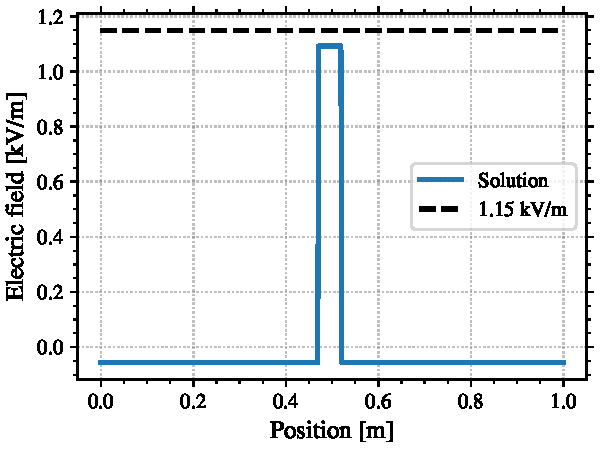
\includegraphics[width=\defaultwidth]{validation_dielectric_field.pdf}
      \caption{Electric field of the capacitor configuration calculated by the Poisson solver in order to validate the discretization and the solver developed. }
      \label{fig-surface}
    \end{figure}



  \subsection{Interface at the cell center}
    In the previous section, we supposed that the plasma-dielectric dielectric boundary was at the interface between the cells.
    However, this means that the electric field close to the interface is unknown, as it is defined at the cell center.
    Moreover, the Dirichlet condition for the potential is better defined at the cell center, and for the sake of simplicity, changing the boundary conditions should not change the particle domain.
    Hence, we chose to position the plasma-wall interface at the center of the cell as shown in \cref{fig-2D,fig-decompo2}.
    This means that the permittivity is not constant over a cell.

    Because the wall boundaries are only in the radial direction, we consider only an interface in the North-South direction.
    \Cref{fig-decompo2} shows the domain decomposition.
    The decomposition is the same as previously, except for the permittivity that can have two different values\string: one in the North half-plane ${\epsr}_{, i,j}^n$ and another in the South half plane ${\epsr}_{, i,j}^s$.

    \begin{figure}[hbt]
      \centering
      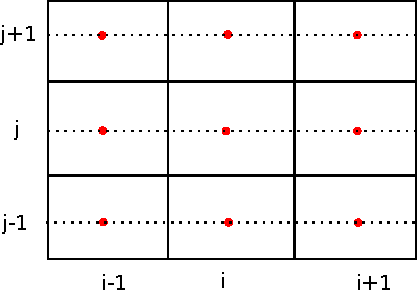
\includegraphics[width=\defaultwidth]{discrect2.pdf}
      \caption{Cartesian decomposition of the \acs{2D} domain. The dash lines represent discontinuities in the permittivity value.}
      \label{fig-decompo2}
    \end{figure}

    The discretization of the Poisson \cref{eq-poissonsum} follows the same path as previously, except that the electric flux in not constant anymore so that \cref{eq-poissonsum} becomes
    \begin{equation}
    \oint_{\C} (-\epsilon \grad \phi) \cdot \vect{n} dS = \sum_{k\in(E,W,N,S)} S^k_{i,j} <\vect{D}^k_{i,j} \cdot \vect{n}>.
    \end{equation}

    We can define
    \begin{align}
    <\vect{D}^E_{i,j} \cdot \vect{n} >&= \frac{1}{2} \epsilon_{i,j}^N E_{x, i+1/2,j}^- + \frac{1}{2} \epsilon_{i,j}^S E_{x, i+1/2,j}^-\\
     &= \frac{-1}{2} (\epsilon_{i,j}^N + \epsilon_{i,j}^S) \frac{\phi_{i+1/2,j} - \phi_{i,j}}{d_i/2}
     \label{eq-flux}
    \end{align}
    so that in the East-West direction, the flux behaves as if the cell permittivity is the mean of the North and South half-plane  $\epsilon_{i,j} = \frac{1}{2} (\epsilon_{i,j}^N + \epsilon_{i,j}^S)$.
    Hence, the rest of the computation is similar.
    For the boundary North and South, the permittivity is constant, hence there is no modification.
    Consequently, we obtain the discretization
    \begin{equation}
    S^E_{i,j} Q^E_{i,j} \phi_{i+1,j} + S^W_{i,j} Q^W_{i,j} \phi_{i-1,j} + S^N_{i,j} Q^N_{i,j} \phi_{i,j+1} + S^S_{i,j} Q^S_{i,j} \phi_{i,j-1} - Q^C_{i,j} \phi_{i,j} = - \V \bar{\rho_{i,j}}
    \label{eq-descretPoissoncentred}
    \end{equation}
    with
    \begin{center}
     $\begin{dcases}
     Q^E_{i,j} &= 2\frac{\epsilon_{i,j} \epsilon_{i+1,j}}{\epsilon_{i,j} d_{i+1} + \epsilon_{i+1,j} d_i} \\
     Q^W_{i,j} &= Q^E_{i-1,j} \\
     Q^N_{i,j} &= 2\frac{\epsilon_{i,j}^N \epsilon_{i,j+1}^S}{\epsilon_{i,j}^N d_{j+1} + \epsilon_{i,j+1}^S d_{j}}\\
     Q^S_{i,j} &= 2\frac{\epsilon_{i,j}^S \epsilon_{i,j-1}^N}{\epsilon_{i,j}^S d_{j+1} + \epsilon_{i,j-1}^N d_{j}} \\
     Q^C_{i,j} &= Q^E_{i,j}S^E_{i,j}+Q^W_{i,j}S^W_{i,j}+Q^N_{i,j}S^N_{i,j}+Q^S_{i,j}S^S_{i,j}
     \end{dcases}$
    \end{center}

    As well as $S^E_{i,j} = S^W_{i,j} =d_id_z, S^N_{i,j} = S^S_{i,j}= d_jd_z$ et $\V = d_jd_id_z$.
    Here, the system is no more symmetric.
    However, we can suppose that the only permittivity jump happens at the cell center, so that  $\epsilon_{i,j}^S = \epsilon_{i,j-1}^N$.
    Hence, $Q^N_{i,j} = 2\frac{\epsilon_{i,j}^N}{ d_{j+1} + d_{j}}$ and the system is symmetric.

  \subsection{Surface charges for centred interface}
    in the case of centred plasma-wall interface, we have surfaces charges at the center of the cell.
    Hence
    \begin{equation}
    \int_{\Omega_{i,j}} \rho dv = \Omega_{i,j}\bar{\rho} + S_{i,j}^N \sigma_{i,j}.
    \end{equation}
    The surface charges behave like volume charges.
    Hence, we obtain
    \begin{equation}
    S^E_{i,j} Q^E_{i,j} \phi_{i+1,j} + S^W_{i,j} Q^W_{i,j} \phi_{i-1,j} + S^N_{i,j} Q^N_{i,j} \phi_{i,j+1} + S^S_{i,j} Q^S_{i,j} \phi_{i,j-1} - Q^C_{i,j} \phi_{i,j} = - \V \bar{\rho_{i,j}} - S^N_{i,j} \sigma_{i,j}
    \end{equation}

    The discretization obtained for the plasma-wall interface cell-centred is very similar to the one obtained for the interface at the cell interface.
    However, it conserves the particle domain when the dielectric layer is not modeled, and that Dirichlet conditions are applied, and the electric field at the plasma-wall interface is better defined.
    Hence, the cell-centred interface will be used.

    \vspace{1em}
    This decomposition has been validate with the same test than presented in \cref{subsec-poisson_validation}.
    We observed no difference between the two decompositions in term of precision.
    
    
  \subsection{Electric field computation}
  
    The resolution of the Poisson equation returns the value of the plasma potential $\phi$ at the cell centers.
    The electric field is computed by taking the first derivative of the potential at the cell interface, as in \cref{eq-flux1},
    \begin{equation} \label{eq-E_ihalf}
      E_{x, i+1/2,j}^- = - \epsilon_{i,j} \frac{\phi_{i+1/2,j} - \phi_{i,j}}{d_i/2},
    \end{equation}
    with $\phi_{i+1/2,j}$ defined with \cref{eq-phidemi1}.
    However, in order to have consistent data, the electric field is also computed at the cell center by interpolation
    \begin{equation} \label{eq-E_mean}
      E_{x, i, j} = \frac{1}{2} \lp E_{x, i-1/2,j} + E_{x, i+1/2,j} \rp =  - \epsilon_{i,j} \frac{\phi_{i+1/2,j} - \phi_{i-i/2,j}}{d_i}.
    \end{equation}
    
    In the cells along to the plasma-wall interface, the effect of the surface charge must be taken into account, is previously described.
    
    \improvement{Can be more explicit here. Add exact expression of $E$ with $\phi_{i,j}$ and the effect of the surface charge.}
  
  
  
% !TEX root=/home/tavant/these/manuscript/src/manuscript.tex

\section{Axial Convection model}
  \label{sec-reinjectionnoise}

  As introduced in the previous section, the \ac{2D} radial-azimuthal simulation does not model a priori the axial convection of the particles.

  \subsection{Lafleur's model of convection}

    \citet{lafleur2016a} proposed a way to model the axial convection of the particles in a \ac{1D} purely azimuthal simulation.
    \Cref{fig-Fake_1d_1} shows a schematic illustration of the model.
    The principle is as follow
    \begin{itemize}
      \item We set a finite axial length, noted $L_z$ on \cref{fig-Fake_1d_1}.
      \item We follow the positions of the particle in the axial direction $z$
      \item When a particle crosses the boundary, it is removed.
      \item A new particle is created
      \begin{itemize}
        \item at $z=0$ for the ions
        \item  at $z=L_z$ for the electrons
      \end{itemize}
    \end{itemize}

    We create a new particle in order to conserve the charge in the simulation.
    The new particle has a velocity following a Maxwellian flux distribution function of a given temperature.
    The azimuthal position of the particle is chosen uniformly at random.

    \improvement{Add definition of the Maxellian and maxellian flux VDF ?}

    \begin{figure}[hbtp]
      \centering
      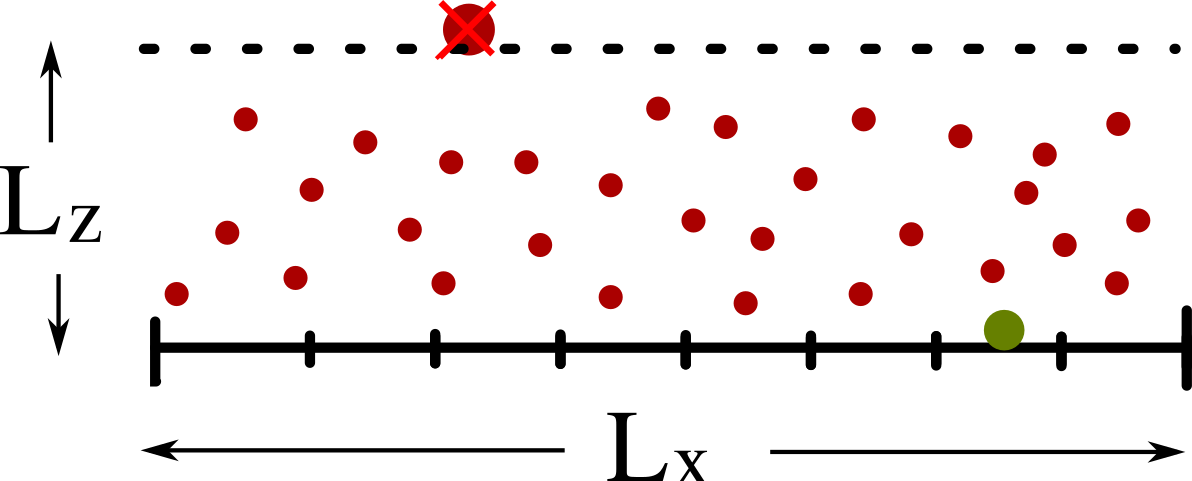
\includegraphics[width=\defaultwidth]{Fake_1d_2}
      \caption{Schematic representation of Lafleur's convection model \citep{lafleur2016a}. The red particle is removed of the simulation, and the green particle is created. In this illustration, the particle is an ion, and the reinjection is at $z=0$. }
      \label{fig-Fake_1d_1}
    \end{figure}

    Lafleur's model of convection has been adopted in \ac{2D} by \citet{croes2017a}.
    The principle is exactly similar.
    The particles are followed in the 3 directions, and a finite length is used to close to axial direction.
    It is important to note that even is the particle are followed in the 3 directions, the meshed domain is only \ac{2D}.
    The simulation is not \ac{3D}-\ac{3V}, but only \ac{2D}-\ac{3V}.

    In \citet{croes2017a}, the authors have observed that if the newly created particle has a radial position chosen uniformly at random, it would affect the sheath.
    Hence, they decided to use the same radial position that the removed particle.
    \Cref{fig-Fake_2d} presents a schematic representation of the convection model in \ac{2D}.

    \begin{figure}[hbtp]
      \centering
      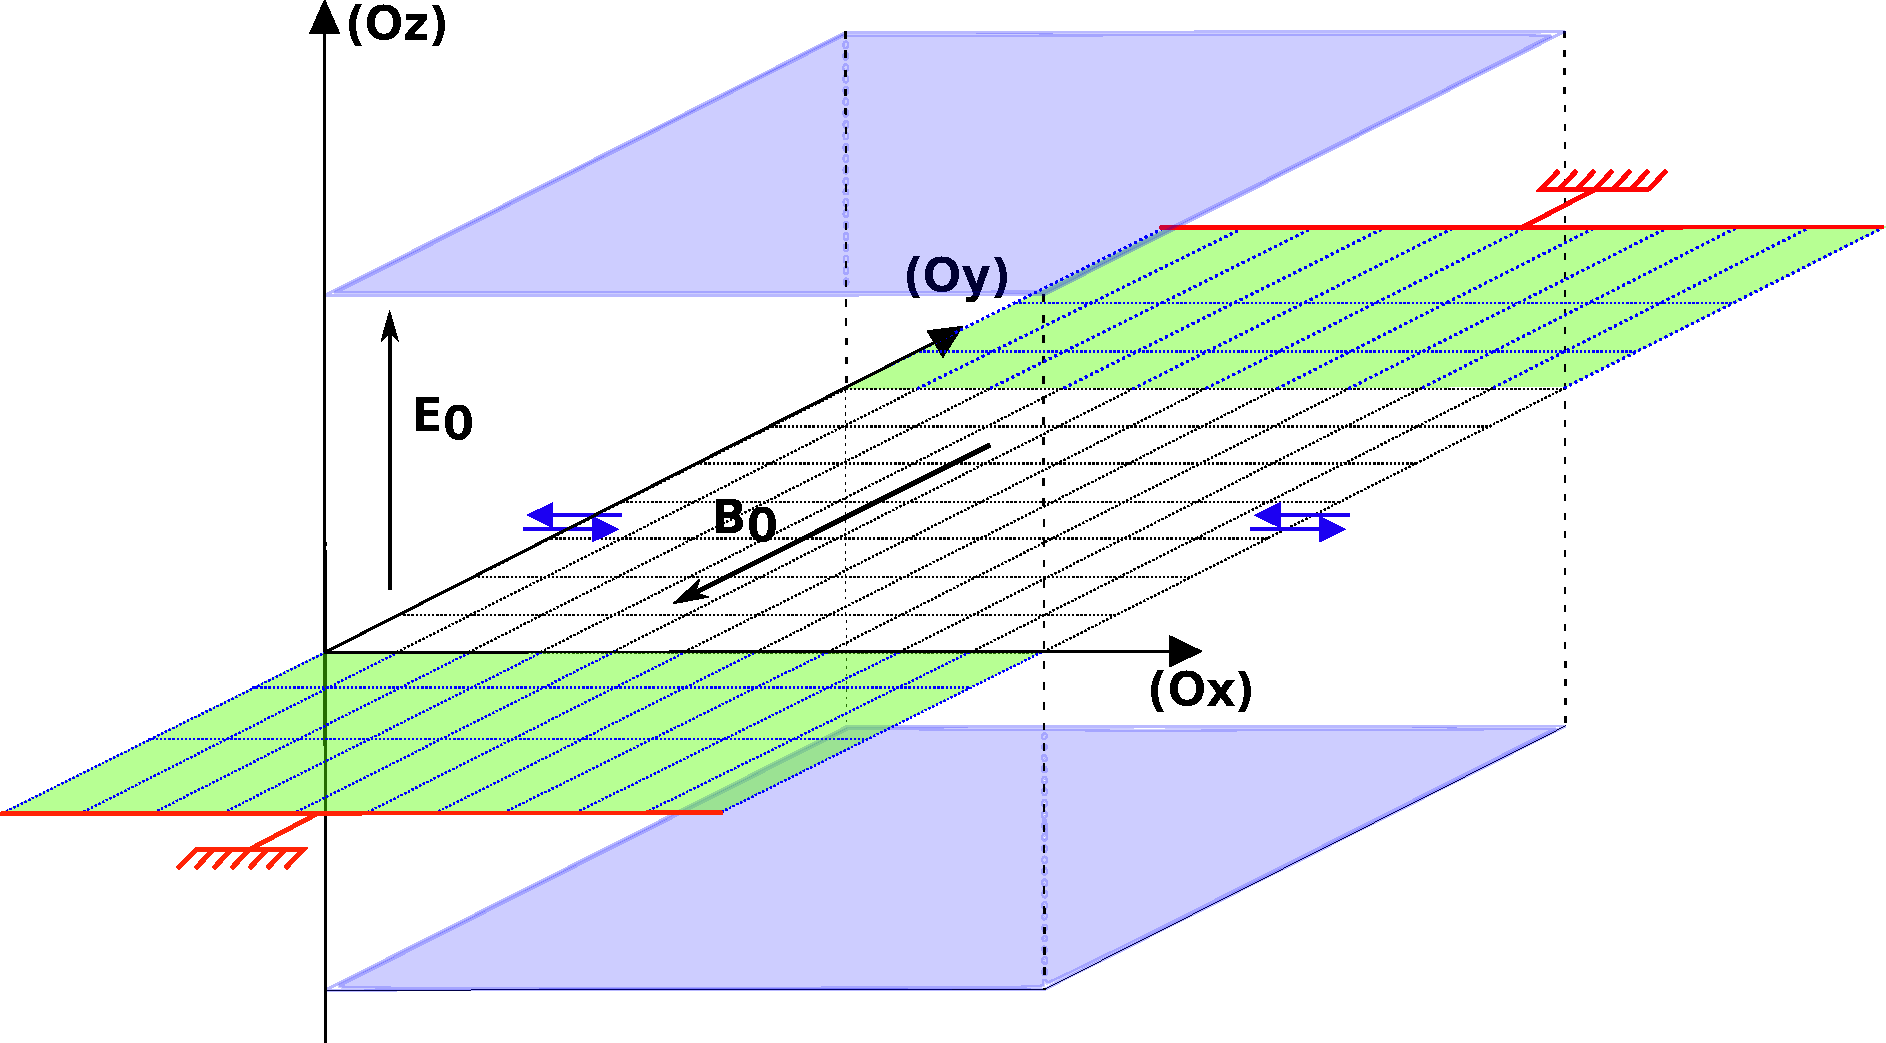
\includegraphics[width=\defaultwidth]{2_5D_dielectric_PPS_small}
      \caption{Schematic representation of the Lafleur's convection model adapted in \ac{2D}. The new particle radial position corresponds to the removed particle, but its azimuthal position is chosen uniformly at random. }
      \label{fig-Fake_2d}
    \end{figure}

    \Cref{fig-energy_convection} shows the evolution as a function of time of the electron mean energy in the simulation in a typical \ac{2D} radial-azimuthal simulation, addapted from \citet{croes2017}.
    We can see that without the convection, the mean energy quickly rises to unphysical values.
    When the convection is modeled, using an axial of $L_z=1$ cm, the energy reaches a steady state.
    \nomenclature[Q]{\ensuremath{ L_z}}{ Axial length}
    \begin{figure}[hbtp]
      \centering
      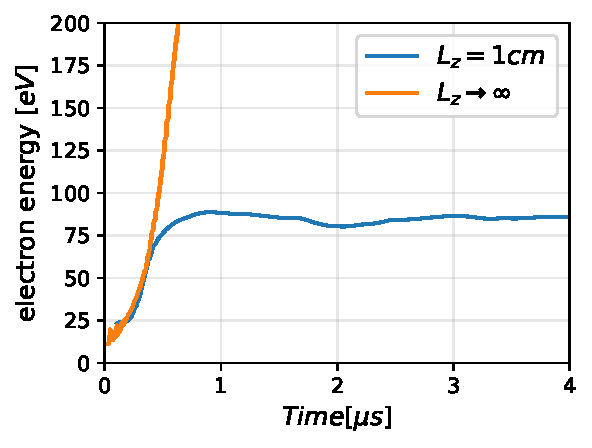
\includegraphics[width=\defaultwidth]{energy}
      \caption{Time evolution of the electron mean energy when the convection is not modeled ($L_z \rightarrow \infty$) and with Lafleur's convection model used, $L_z = 1$ cm. Adapted from \citet{croes2017}.}
      \label{fig-energy_convection}
    \end{figure}



  \subsection{Numerical artefacts}
    \citet{lafleur2016a} studied the impact of the convection model on the simulation results.
    The authors observed in particular that changing the azimuthal length of the simulation domain could affect the simulation results.

    \Cref{fig-convection_numerical} shows the time evolution of the azimuthal electric field $E_{\theta}$ from the \ac{1D} simulation \citep{lafleur2016a}.
    \nomenclature[Q]{\ensuremath{ E_{\theta}}}{ Azimuthal electric field}

    On the first row (\cref{fig-convection_numerical}.{\bf a} and {\bf b}), the length of the periodic azimuthal direction is $L_{\theta}=0.5$~cm.
    \cref{fig-convection_numerical}.{\bf a} corresponds to the case without axial convection.
    We clearly see that the \ac{ECDI} rises and does not saturate.
    The wavelength is short, of the order of $\lambda = 1.5$~mm.
    \nomenclature[Q]{\ensuremath{ \lambda}}{ Wave length}
    \cref{fig-convection_numerical}.{\bf b} corresponds to the same case as \cref{fig-convection_numerical}.{\bf a} but this time with the axial convection modeled.
    We observe this time a saturation of the oscillation's amplitude, and the wavelength is close to $\lambda \simeq 1.5$~mm.

    On the second row (\cref{fig-convection_numerical}.{\bf c} and {\bf d}), the length of the periodic azimuthal direction is $L_{\theta}=1$~cm.
    \cref{fig-convection_numerical}.{\bf c} corresponds to the case without axial convection, and \cref{fig-convection_numerical}.{\bf b} corresponds to the same case but with the axial convection modeled.
    In \cref{fig-convection_numerical}.{\bf c}, we can see that increasing the azimuthal length did not affect the \ac{ECDI}, as expected.
    However, in  \cref{fig-convection_numerical}.{\bf d}, the instability is clearly affected.
    A single oscillation is observed, corresponding to $\lambda=10$~mm, which seems almost certainly unphysical.

    \begin{figure}[hbtp]
      \centering

      \begin{tabular}{cc}
        \subfigure{Lafleur_NoLz_1}{a}{20, 20}
            &
        \subfigure{Lafleur_Lz_1}{b}{20, 20} \\

        \subfigure{Lafleur_NoLz_2}{c}{20, 20} &
        \subfigure{Lafleur_Lz_2}{d}{20, 20} \\
      \end{tabular}
      \caption{Effects of Lafleur's convection model for two different azimuthal length on the azimuthal electric field. ({\bf a}) No convection, $L_x=0.5$~cm,  ({\bf b}) convection modeled, $L_x=0.5$~cm,  ({\bf c}) No convection, $L_x=1$~cm,  ({\bf d}) convection modeled, $L_x=1$~cm. The colour of each plots is normalized to the maximum amplitude. Adapted from \citep{lafleur2016a}. \inlinenote{Get $\theta$ back to $y$ instead of $x$}}
      \label{fig-convection_numerical}
    \end{figure}

    \FloatBarrier
    \citet{croes2017} observed similar behaviour with the bidimensional  simulation.
    The author investigated the values of the azimuthal length which presented physical and unphysical results
    for different values of the axial length.
    \Cref{fig-couplesCroes} shows the results obtained (adapted from \citep{croes2017}).
    We can see that for a given value of the axial length, the azimuthal must be less that a certain value to present physical results.
    However, the value of this upper limit depends of the axial length, such that the if the axial length decreases, the upper limit of the azimuthal length decreases as well.

    \begin{figure}[hbtp]
      \centering
      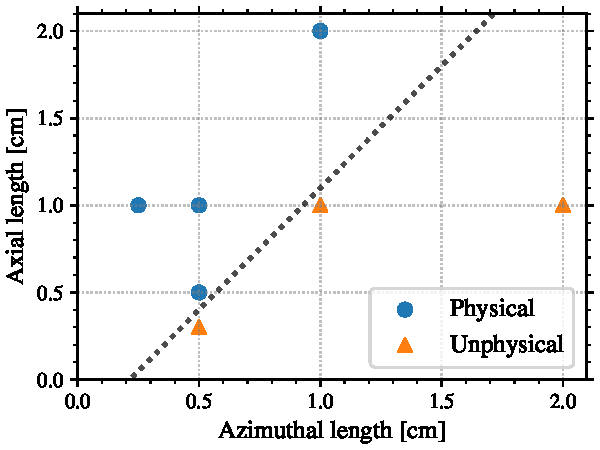
\includegraphics[width=\defaultwidth]{2D_couples}
      \caption{Values of the azimuthal length and the axial length for which the simulation result is physical (similar to \cref{fig-convection_numerical}.{\bf b}) or unphysical  (similar to \cref{fig-convection_numerical}.{\bf d}) \inlinenote{Make this image smaller (smaller font, etc.), correct azimuthal}}
      \label{fig-couplesCroes}
    \end{figure}

    In the next section, we develop a theory that could explain the observation, and a new convection model for the simulation is proposed.

  \subsection{Numerical noise of Lafleur's convection model}

    Let us consider Lafleur's convection model in \ac{1D} on the charge density.
    When computing the charge density on the mesh vertices, the axial position is not taken into account.
    Consequently, the convection process illustrated on \cref{fig-Fake_1d_1} is similar to moving a particle arbitrarily (read randomly).
    Seen by the charge density, this is similar to a Poisson noise, also named shot noise, on the charge density.\footnote{Actually, this noise is the combination of a Poisson noise with a uniform noise, happening twice for every particles convection, once with a positive charge and once with a negative charge.}

    After a certain number of particles removed and created, the Poisson noise is similar to a Gaussian noise, also named thermal noise, following a normal distribution $\N$ . 
    \nomenclature[Q]{\ensuremath{ \N }}{ Normal distribution.}
    Hence, the charge density becomes \footnote{One can note that the mean of the noise is strictly zero (with probability 1), as the charge density is conserved.}
    \begin{equation} \label{eq-rhonoise}
      \rho = \rho_0 + \N(0, \stdconv),
    \end{equation}
    with $\rho$ the charge density, $\rho_0$ the charge density without the convection process, and $\stdconv$ the standard deviation of the distribution of the noise associated with the convection model.
    \nomenclature[Q]{\ensuremath{ \rho}}{ Charge density}
    \nomenclature[Q]{\ensuremath{ \stdconv}}{ tandard deviation of the distribution of the noise associated with the convection model}
    Surprisingly, the noise due to the convection model is similar to the numerical noise induced by the decomposition of the plasma into particles $\N(0, \sigma_{\rm stat})$.
    However, the amplitude of this statistical noise decreases with the number of particles per cell used
    \begin{equation*} \label{eq-statistical}
     \sigma_{\rm stat} \propto \frac{1}{\sqrt{N_{pc}}}.
    \end{equation*}

    On the other hand, the amplitude of the noise induced by the convection model depends on the plasma density $n$, the axis velocity of the particles $v_z$ and the axial length $L_z$
    \begin{equation} \label{eq-convstd}
     \stdconv \propto \frac{n}{L_z} v_z.
    \end{equation}

    We can see on \cref{eq-convstd} that the amplitude of the convection induced noise on the charge density is proportional to the inverse of the axial length $L_z$.
    This could explain the observation of \cref{fig-couplesCroes} when using a smaller $L_z$.
    However, it does not explain the effects of the azimuthal length observed in \cref{fig-couplesCroes,fig-convection_numerical}.

  \subsection{Effect of the noise on the electric field}
    \label{sec-mathnoise}
    In order to explain the impact of the azimuthal length on the instability, we can study the azimuthal electric field $\aziE$ resulting of the charge density $\rho$.
    As the Pouisson equation is linear, we have
    \begin{align}
      \aziE(\theta) &= C + \frac{1}{\epsilon_0} \int_0^{\theta} \rho(s) ds\\
                    &= C + \frac{1}{\epsilon_0} \int_0^{\theta} (\rho_0(s) + \N(0, \stdconv) ) ds \\ 
                    &= C + \aziE_{, 0} + \aziE_{, 1}
    \end{align}
    with $C$ a constant that ensure that the periodical \ac{BC} are respected.
    The part of the electric field $\aziE_{, 0}$ corresponds to the unperturbed charge density $\rho_0$ and $\aziE_{, 1}$  corresponds to the noisy charge density $\N(0, \sigma_{\rm stat})$.
    Hence, let us focus now on $\aziE_{, 1}$.
    We can study $\aziE_{, 1}$ using two equivalent means\string: the \ac{FT} and the Brownian bridge.
    
    \paragraph{Fourier Transform \\}
      Applying the \ac{FT} on the equation
      \begin{equation} \label{eq-aziE1}
        \aziE_{, 1} = \frac{1}{\epsilon_0} \int_0^{\theta}  \N(0, \stdconv) ds
      \end{equation}
      gives    
      \begin{align}
        \FFT \lp \aziE_{, 1} \rp (k) &= \frac{1}{\epsilon_0} \FFT \lp \int_0^{\theta}  \N(0, \stdconv) ds \rp \\
                                     &= \frac{1}{\epsilon_0} \frac{ \N(\mu_{\rm FT}, \sigma_{\rm FT})}{k} \label{eq-fft}
      \end{align}
      
      \Cref{eq-fft} shows that $\aziE_{, 1}$ is also follows a Gaussian distribution, but with a non-zero mean value.
      It is also inversely proportional to the wave number $k$.
      Hence, when we increase the azimuthal length, which means that small wave number can exit in the simulation domain, the amplitude of $\aziE_{, 1}$ increases as well.
      
    \paragraph{Brownian Bridge\\}
      \Cref{eq-aziE1}, combined with the \ac{BC}, is the definition of the a Browning bridge.
      
      A Brownian bridge is a particular Brownian motion that reaches at a given distance the same value that the initial value.
      Hence, we have \citep{ibe2013}
      \begin{align*}
        \mathbb{E}(\aziE_{, 1}) &= 0,  \\
        {\rm var}(\aziE_{, 1}) &= \stdconv^2 \frac{L_{\theta}}{4}
      \end{align*}
    
      Hence, the increase of the azimuthal length increases the amplitude of $\aziE_{, 1}$.
      
    
    We believe that when the amplitude of $\aziE_{, 1}$ is too large, it can trigger an unphysical oscillation.
    The next section uses this conclusion in order to adapt the convection model.
    
    \subsection{Noiseless convection model}
      \label{sec-noiselessresults}
      In previous section, we have shown that the convection model induces a noise in the charge density, that produces an azimuthal electric field which amplitudes depends on the azimuthal length.
      
      We propose here a modified version of Lafleur's convection model in order to remove the noise in the charge density
      The noiseless convection model follows the same algorithm that before, but the azimuthal position of the particle created is not chosen uniformly as random, but instead the new particle has the same position as the removed particle.
      \Cref{fig-fakez3} shows a schematic illustration of the noiseless convection algorithm applied on a particle.
      
      \begin{figure}[hbtp]
        \centering
        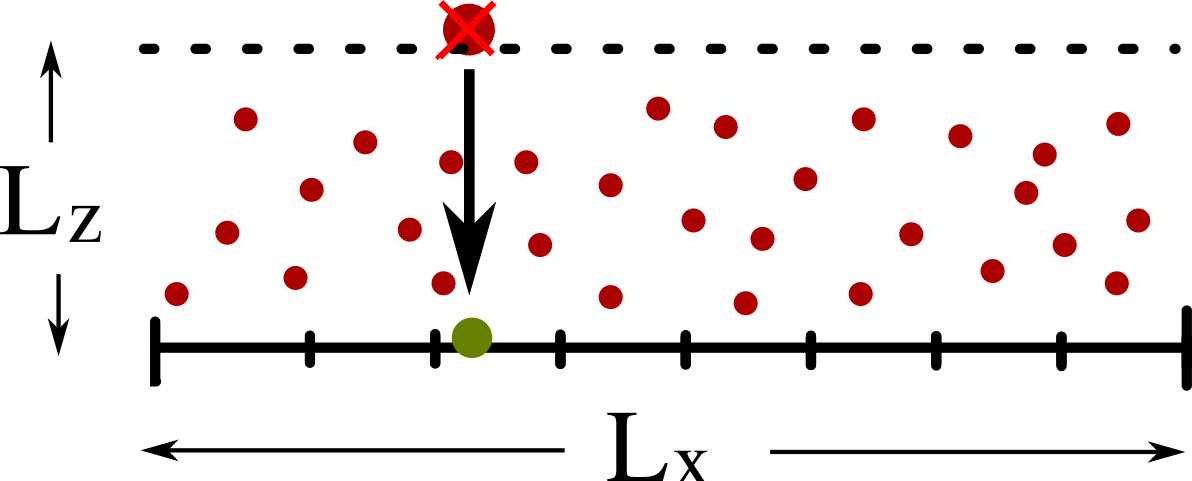
\includegraphics[width=\defaultwidth]{Fake_1d_3}
        \caption{Illustration of the noiseless convection model}
        \label{fig-fakez3}
      \end{figure}
      
      We have implemented this modified convection model in the \ac{2D} radial-azimuthal simulation.
      
      \Cref{fig-newconv_noconv} shows the time  evolution of the azimuthal electric field at the center of the radial dimension with and without the noiseless convection model.
      It presents the same conditions that in \cref{fig-convection_numerical}.{\bf a} and {\bf b}. 
      As previously, the convection stabilises the growth of the instability to a steady-state, but it does not affect the physics.
       
      
      \begin{figure}[hbtp]
        \centering
        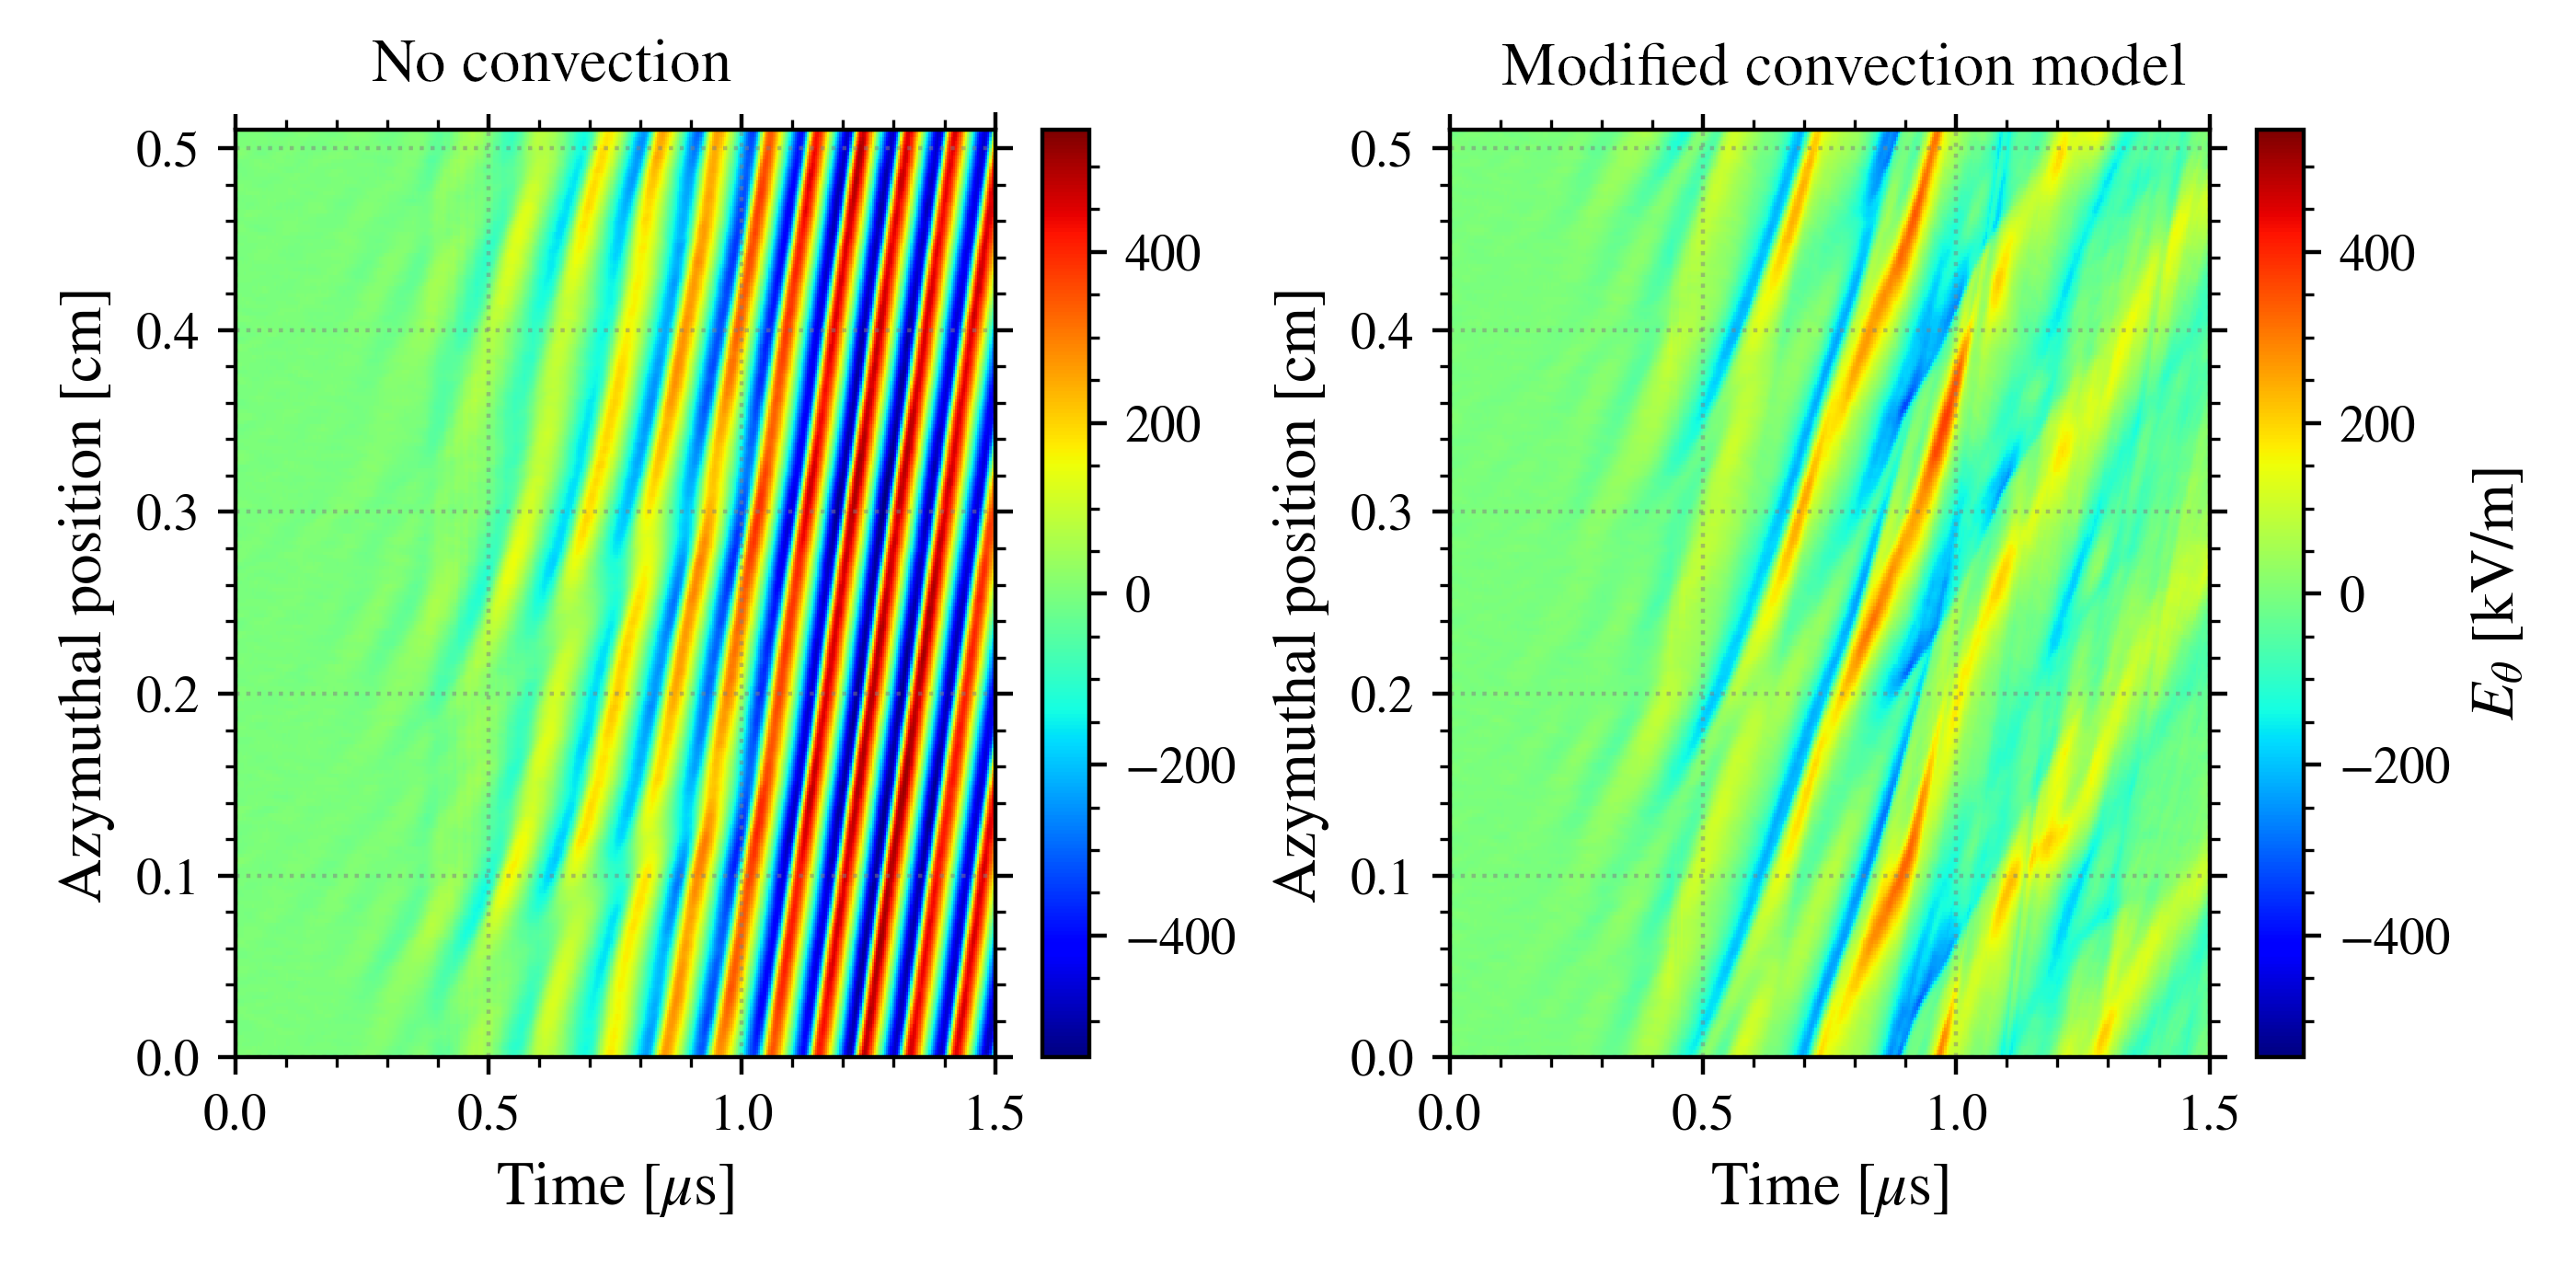
\includegraphics[width=\defaultwidth]{Compare_no_new_Reinj_Oz}
        \caption{Time evolution of the azimuthal electric field at the center of the radial dimension with and without the noiseless convection model. }
        \label{fig-newconv_noconv}
      \end{figure}
      
      \Cref{fig-oldeconv_newconv} shows the  time  evolution of the azimuthal electric field at the center of the radial dimension  with the convection modeled using Lafleur's model and the noiseless model with a small azimuthal length.
      We can see that the two models gives almost exactly the same results.
      
      \begin{figure}[hbtp]
        \centering
        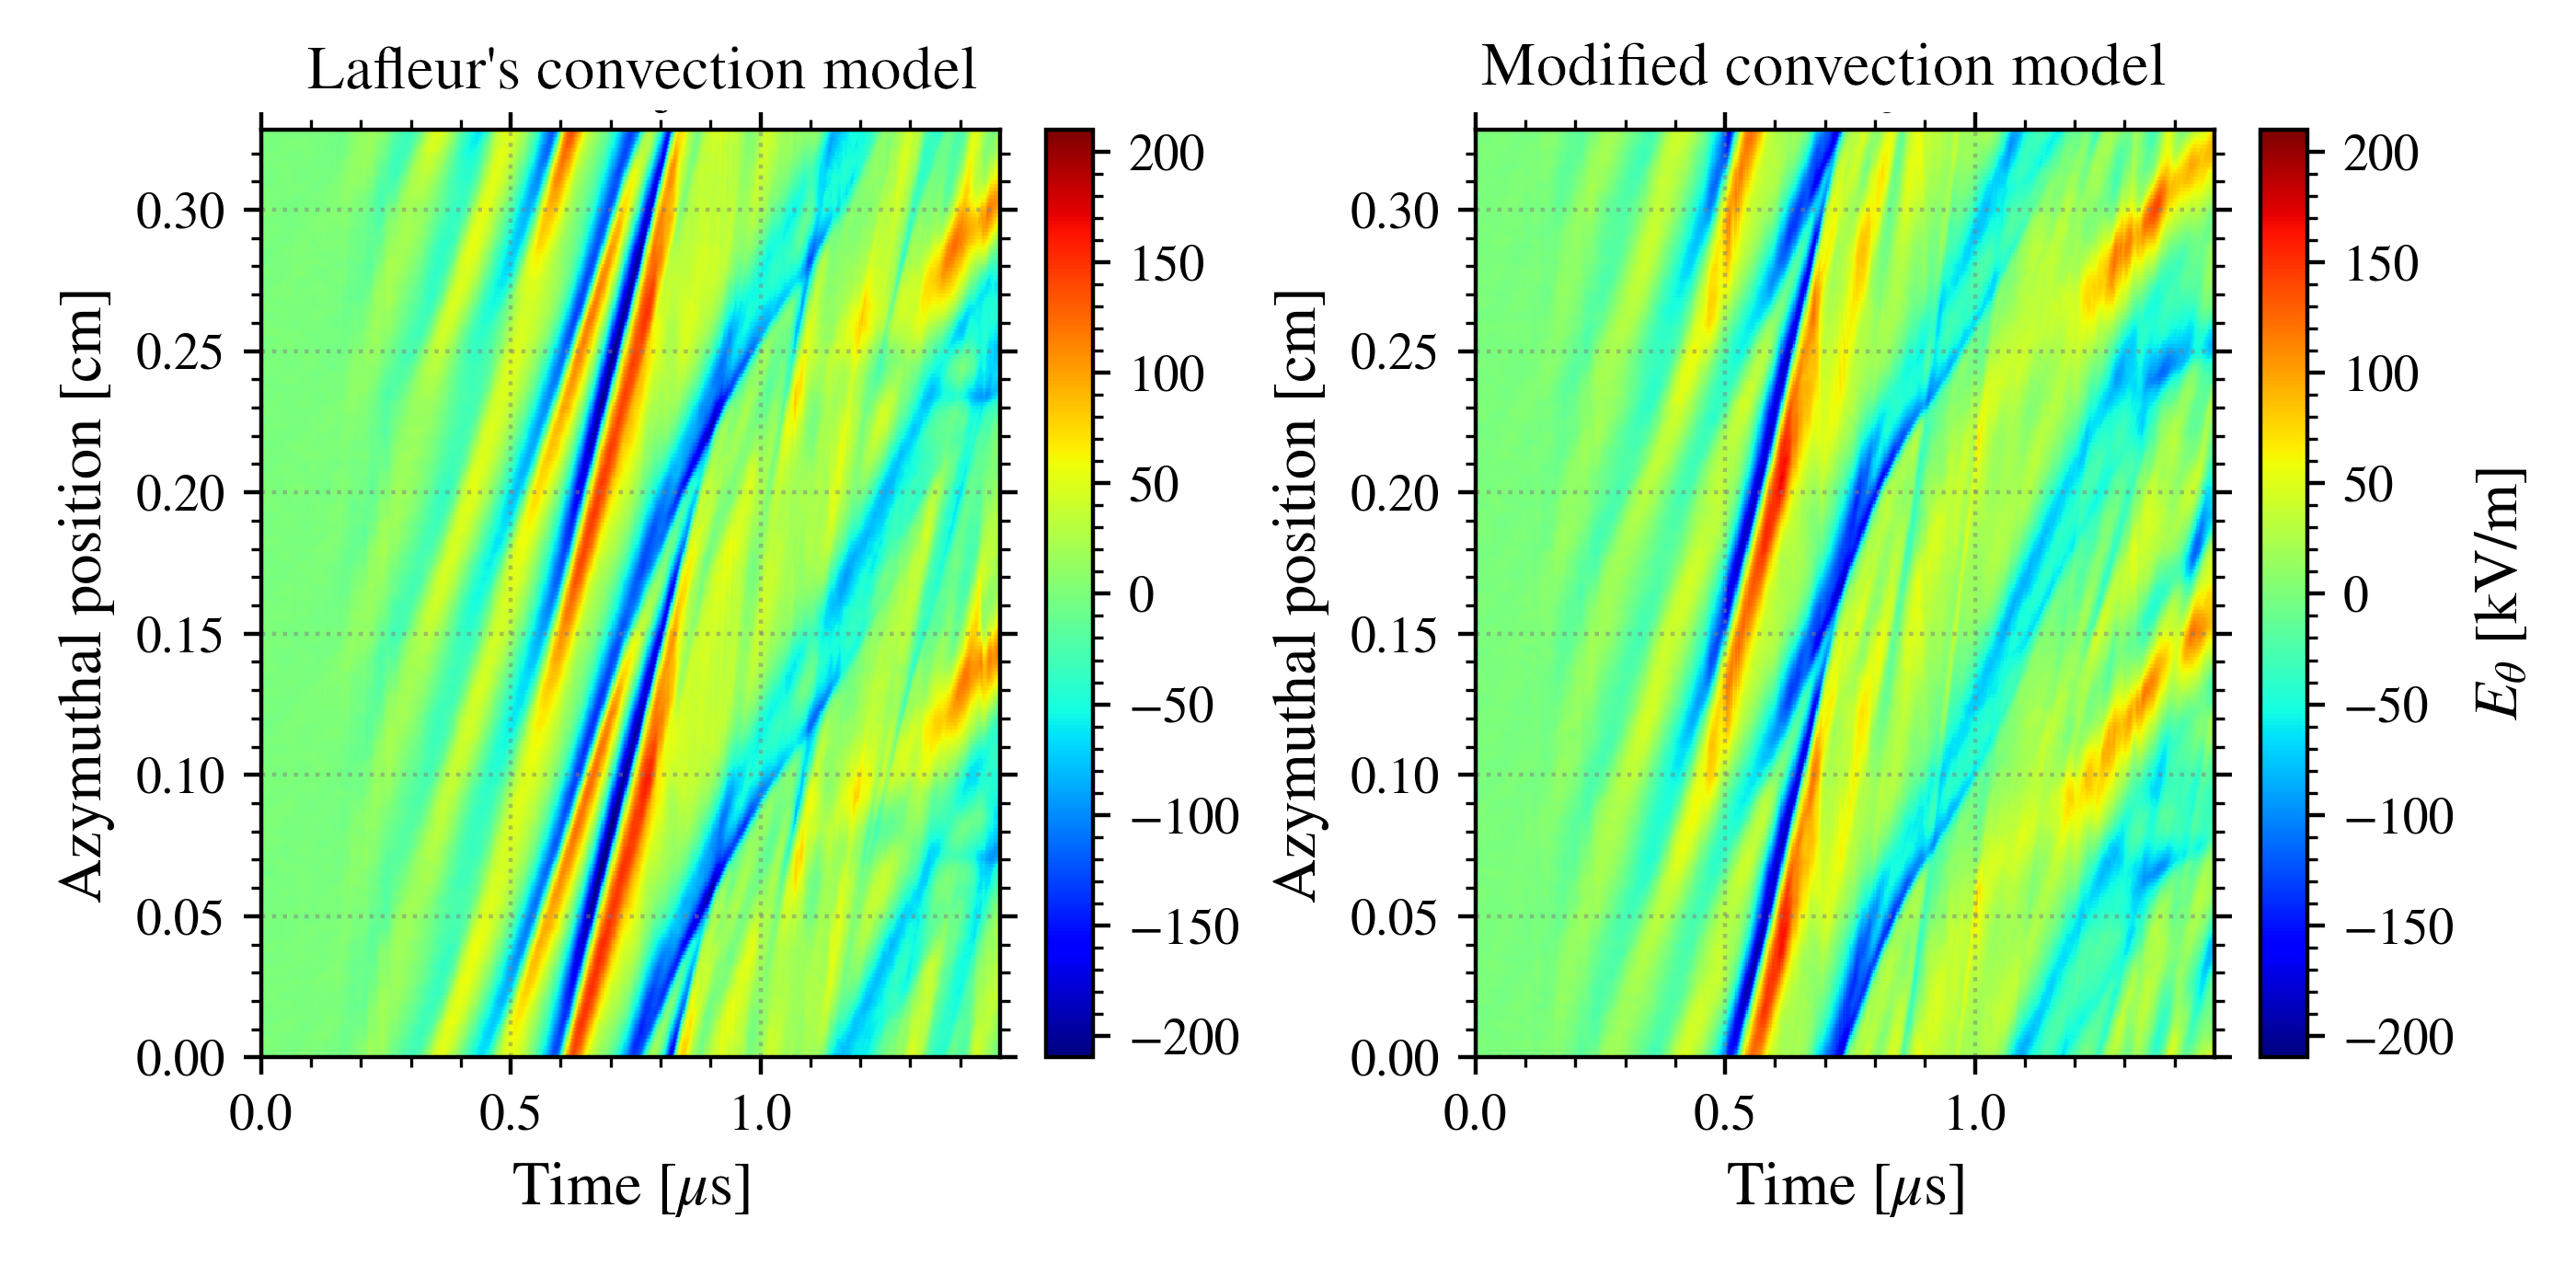
\includegraphics[width=\defaultwidth]{Compare_old_new_Reinj_Oz}
        \caption{Time evolution of the azimuthal electric field at the center of the radial dimension with the convection modeled using (left) Lafleur's model and (right) the noiseless model with a small azimuthal length.}
        \label{fig-oldeconv_newconv}
      \end{figure}
      
      
      \Cref{fig-oldeconv_newconv_longLZ} shows the  time  evolution of the azimuthal electric field at the center of the radial dimension  with the convection modeled using Lafleur's model and the noiseless model but using a longer azimuthal length than \cref{fig-oldeconv_newconv}.
      In this cases, we can see that Lafleur's convection model induces oscillations that are not observed with the noiseless model.
      
      \begin{figure}[hbtp]
        \centering
        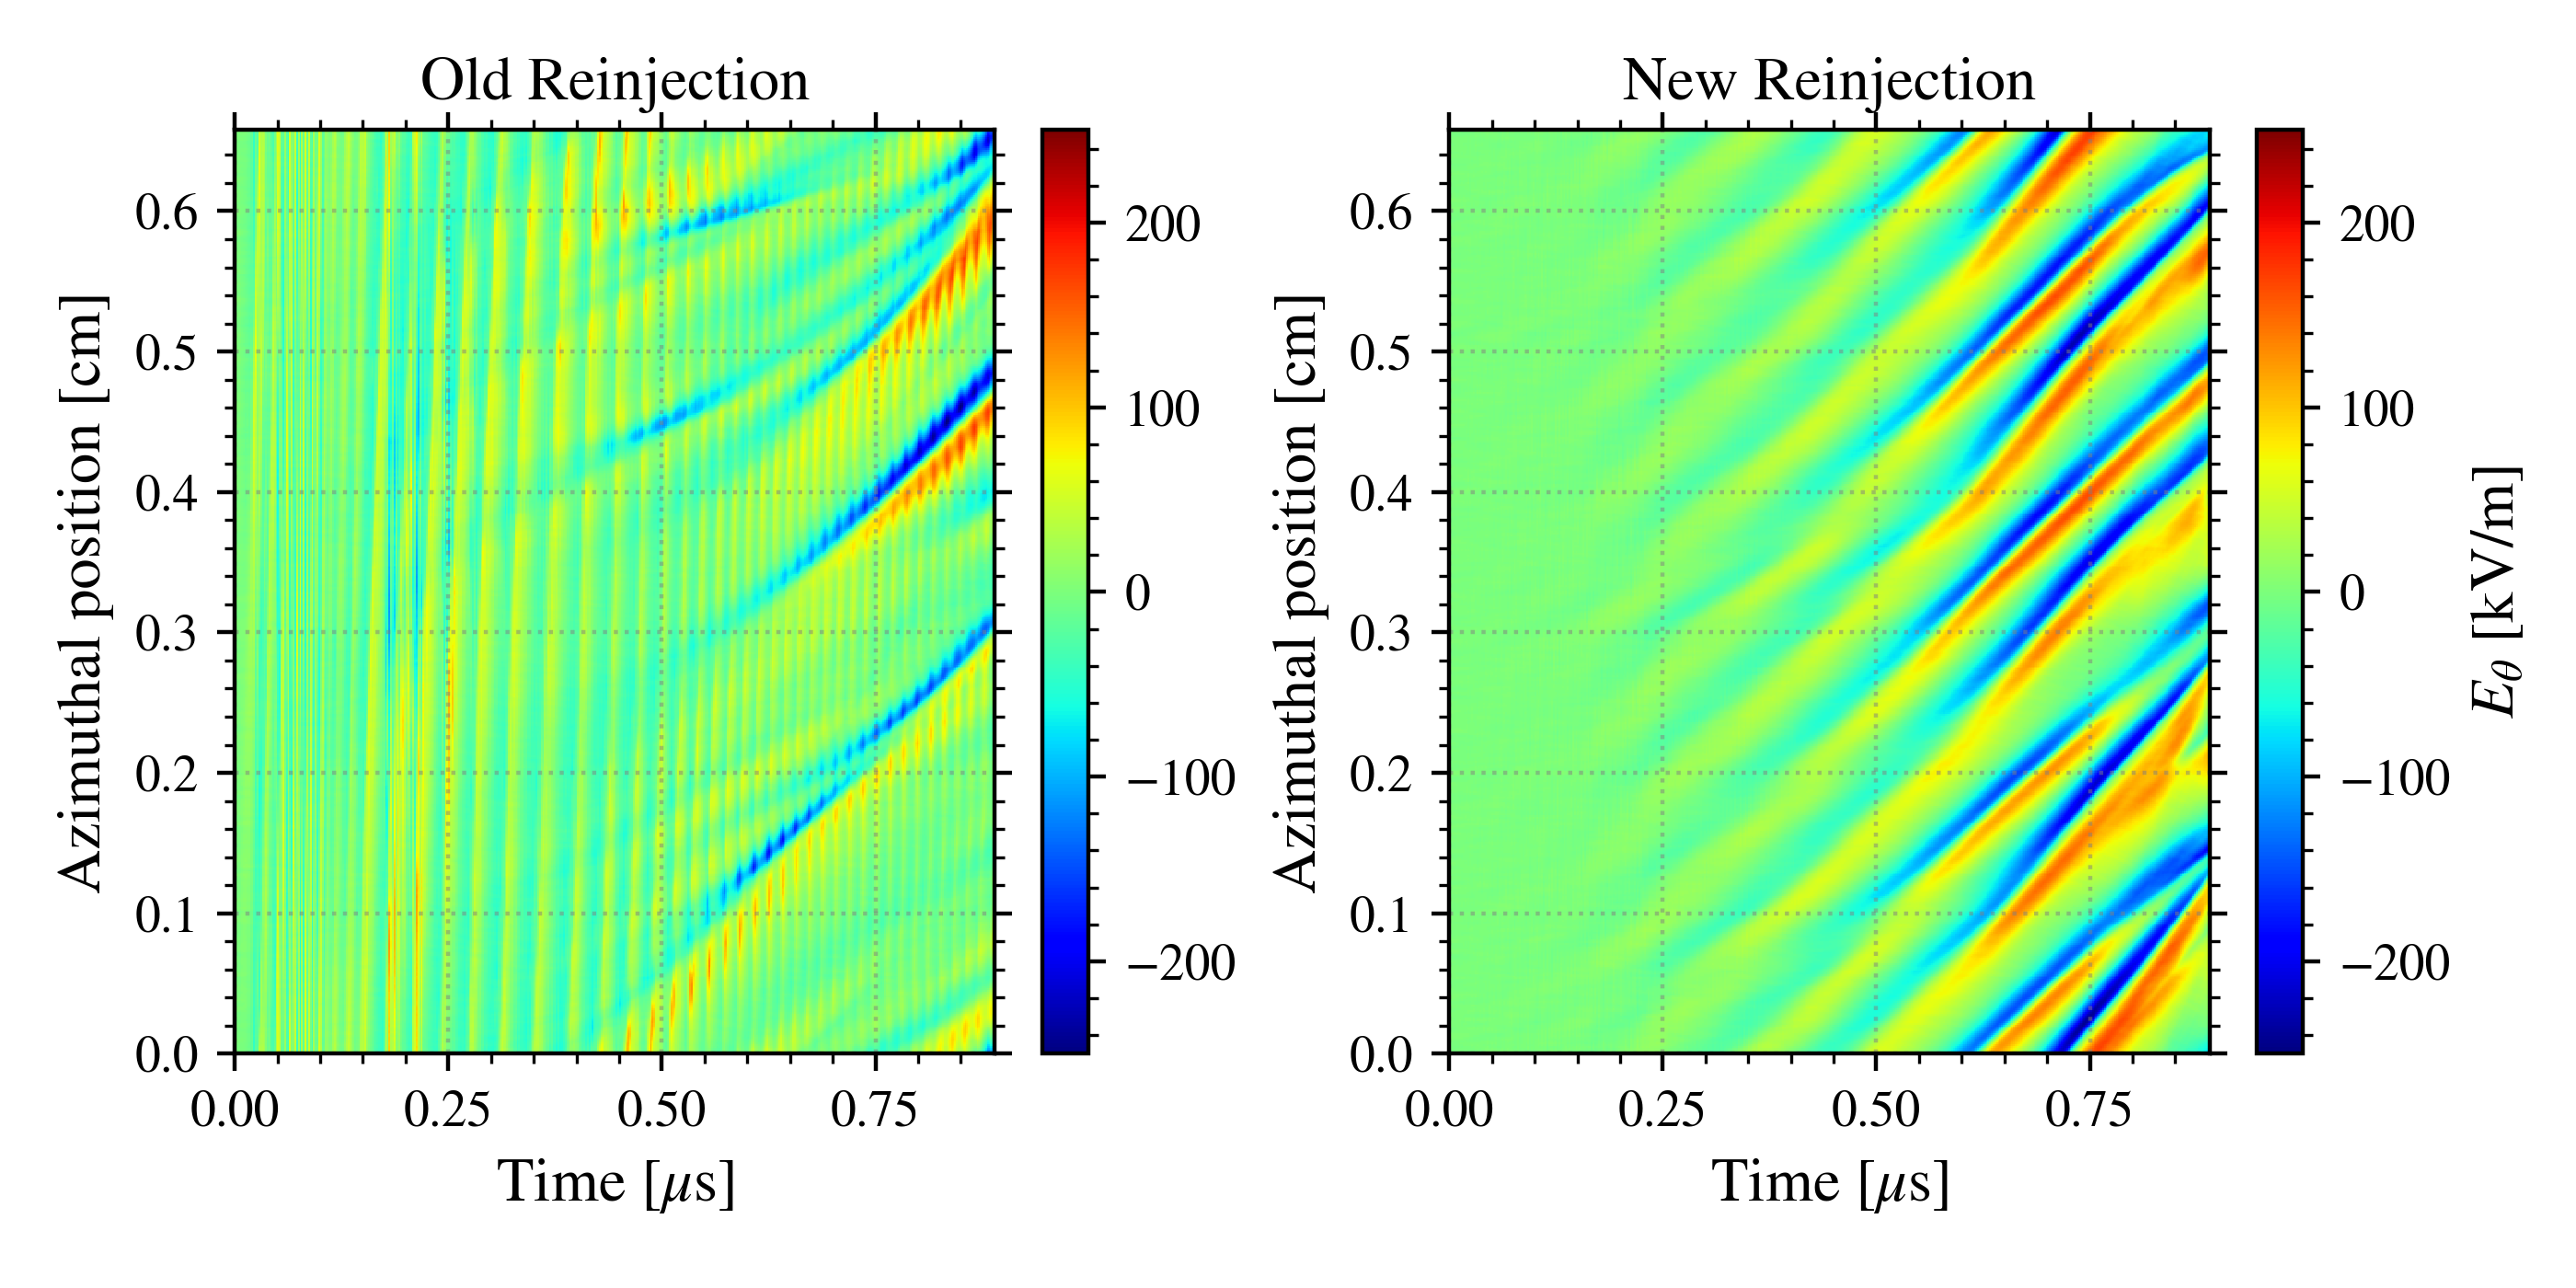
\includegraphics[width=\defaultwidth]{Compare_old_new_Reinj_Oz_LongLx}
        \caption{Time evolution of the azimuthal electric field at the center of the radial dimension with the convection modeled using (left) Lafleur's model and (right) the noiseless model with a longer azimuthal length.}
        \label{fig-oldeconv_newconv_longLZ}
      \end{figure}
      


      Theses observations have shown that Lafleur's convection model induces a noise on the charge density, that do not affect the simulation when the domain size is small, but can rise numerical artefacts when the domain size is larger.
      We have seen that the minor modification on the model do not affect the simulations results on a small domain, but allow us to use larger simulation domain without any numerical artefacts.
      
      Unfortunately, the new model has been developed during the last year of my theses.
      Hence, the first simulation results have been obtained using Lafleur's convection model.
      As seen in \cref{fig-oldeconv_newconv}, on a small geometry the results are not affected, hence there is no need to verify all of the simulations obtained.
      On the other hand, in order to study the instability, it is useful to have a longer azimuthal, in order to obtain a more resolved frequency spectra.
      Hence, the modified convection model  used in this case.
      \inlinenote{Give precise sections where it is used}
          
    \subsection{Effects on a \ac{2D} simulation domain}
      
      The mathematical development of \cref{sec-mathnoise} has been done in \ac{1D}.
      We can legitimately wonder is the results  can be extended directly to a \ac{2D} domain.
      A mathematical definition of $\aziE_{, 1}$ is more difficult, as we have, neglecting the dielectric layers,
      \begin{equation} \label{eq-aziE}
        \aziE_{, 1} = \partial_{\theta} \phi_1 \text{ such that } \grad \cdot \grad \phi_1 = - \frac { \N(0, \stdconv)}{\epsilon_0} \text{ following the \ac{BC}}.
      \end{equation}
      The \ac{BC}s are
      \begin{itemize}
        \item periodic \ac{BC} in the azimuthal direction,
        \item Dirichlet \ac{BC} in the radial direction, modeling grounded walls,
      \end{itemize}
      which translate as
      \begin{align}
        &\phi = 0 \text{ for } r=0 \text{ and } r=L_r, &\forall \theta \label{eq-BC1} \\
        &\phi(\theta = 0)= \phi(\theta = L_{\theta}) , &\forall r \label{eq-BC2}
      \end{align}
      
      Solving \cref{eq-aziE,eq-BC1,eq-BC2} analytically is much more difficult that the \ac{1D} development because of the Dirichlet \ac{BC}.
      \nomenclature[N]{Dirichlet Boundary condition\string:}{ a type of boundary conditions for which the field is fixed. For instance for grounded electrodes on the plasma potential\string: $\phi = 0$}
      However, we can investigate it numerically, by solving \cref{eq-aziE} for a given random source term.
      Using a Monte Carlo approach, the results are averaged 50 times in order to better observe the mean behaviour in respect to the noise (i.e. increasing signal to noise ratio).
        
      \Cref{fig-dftLr} shows the \ac{DFT} of the source term \[\rho_1 = \N(0, \stdconv),\] the resulting azimuthal electric field $\aziE_{, 1}$ and plasma potential $\phi$ computed on the centreline of the simulation domain in the radial direction, for three different radial length expressed in number of cell $N_x$.
      Is also showed the "equivalent" source term $\rho_{\rm eq}$, which is the source term that would give the frequency spectra of $\aziE_{, 1}$ observed in a \ac{1D} domain
      
      \begin{equation} \label{eq-equirho}
        \rho_{\rm eq} = \epsilon_0 \partial_\theta \aziE_{, 1}.
      \end{equation}
      The results are given for different radial length $N_x=15,50 \text{ and } 200$, while the azimuthally length $N_y=200$ is kept constant.
      We can see that the plasma potential and the electric field show larger amplitude for small wave numbers (large wavelength) compared to large wave numbers in the three cases.
      However, the amplitude of the smaller wave numbers is affected.
      In the cases of small radial length ($N_x=15 \text{ and } 50$), the spectra of the electric field is not monotonic.
      This can be explained by the Dirichlet \ac{BC}s that {\it pin down} the fluctuation of the plasma potential.
      
      However, even though the amplitude is reduces in \ac{2D} with small radial direction compared to a \ac{1D} model, we still observe large amplitude of small wave number oscillations in both the electric field and the plasma potential.
      Hence, the conclusions of  \cref{sec-mathnoise} derived in \ac{1D} can be legitimately used for \ac{2D} domains.
      
      
      
      \begin{figure}[hbtp]
        \centering
        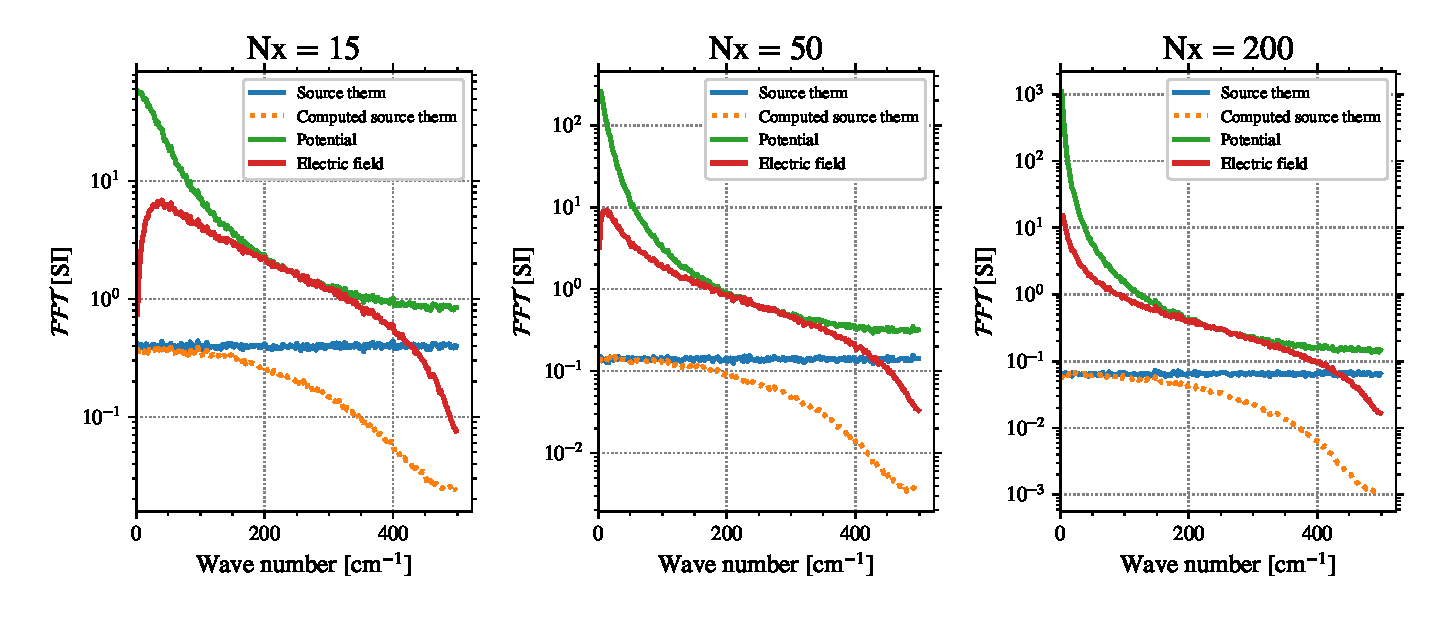
\includegraphics[width=\textwidth]{effect_Lr}
        \caption{\ac{DFT} of the source term $\rho_1 = \N(0, \stdconv)$, the resulting azimuthal electric field $\aziE_{, 1}$ and plasma potential $\rho$ computed on the centreline of a radial-azimuthal simulation, and the "equivalent" source term defined by \cref{eq-equirho}. $N_y=200$. }
        \label{fig-dftLr}
      \end{figure}
      
      






% !TEX root=/home/tavant/these/manuscript/src/manuscript.tex

\section{Secondary electron emission}
\label{sec-seemodel}
When an incident electron reaches the wall material, several scenarii are possible, as described in \citet{villemant2018}
\begin{enumerate}
  \item Elastic reflection\string: the electron encounters only elastic collision with the material, hence its energy is constant. However, its reflection is not necessary specular.
  \item Inelastic reflection\string: the electron looses some of its energy to the material before returning to the plasma.
  \item Secondary electron emission\string: the energy of the primary electron is enough to extract one or more electrons from the material.
  \item No emission, the electron is absorbed by the wall.
\end{enumerate}

The probability \proba{}  that one event happens instead of another depends predominantly on the particle energy, and weakly on its  impact angle.
Concerning the mean flux of electron incident and emitted, we uses the mean emission rate, or yield, \rate
\begin{equation*} \label{eq-ratedifinition}
  \rate = \frac{\Gamma_{e, \rm secondary}}{\Gamma_{e, \rm primary}}
\end{equation*}
which can be developed using the distribution function to 
\begin{equation*} \label{eq-ratedifinition_evdf}
  \rate = \frac{\iiint_{\Omega} v_x \proba(\vect{v_e}) f(\vect{v_e}) d^3v}{\iiint_{\Omega} v_x \proba(\vect{v_e}) f(\vect{v_e}) d^3v}
\end{equation*}
with $\Omega$ the ensemble of $\vect{v_e}$ directed toward the wall\string: $\vect{v_e} \cdot \vect{n} > 0$, with $\vect{n} $ the unit vector normal to and toward the wall.

\subsection{Models of emission } \label{subsec-seemodels}
Several models can be used to describe the electron emission.

\paragraph{Monte Carlo models} are the more realistic.
 They are based on the computation of the trajectory of the electrons through the material, during which the electron can encounter several interactions with the material.
 Each interactions can modify the electron direction, energy, and generate new electron.
 Several models have been proposed, as \citet{furman2002,pierron2017}.
 These models allow a precise characterization of the processes, but depends of a large number of parameters difficult to obtain due to the lack of experimental data.
 
\paragraph{Analytical models} provides a simplified description of the rate of emission.
Their complexity depends of the precision desired.
The most largely used are the models of \citet{vaughan1989,barral2003a,sydorenko2006b}.

In this work, we are interested only in representing qualitatively the electron emission.
Moreover, \citet{croes2017} showed that changing the model used do not affect significantly the results. 
Hence, we will use the model of \citet{barral2003a} for its simplicity.

\subsection{Barral electron emission model}
\label{sec-modelused}

The emission model used follows a linear-saturated law for the probability of emission with three parameters. 
It describes the total emission corresponding to the sum of the elastic and inelastic backscattering and the secondary electron emission.
\begin{equation} \label{eq-proba_barral}
  \proba(\ek) = 
  \begin{cases}
    \proba_0 + (1 - \proba_0) \frac{\ek}{\crover}   &\text{ if } \ek <  \ek_{\max} \\
    \probamax &\text{ if } \ek \geq \ek_{\max}
  \end{cases}
\end{equation}
where $\ek$ is the kinetic energy of the incoming electron, $\proba_0$ is the asymptotic probability of emission at energy null, $\crover$ is the crossover energy above which the probability of emission is higher that one, \probamax is the maximum probability and $\ek_{\max}= \frac{\probamax - \proba_0}{1 - \proba_0} \crover $ is the minimum energy for which $\rate = \probamax$ .
\Cref{eq-proba_barral} is illustrated in \Cref{fig-modelbarral}.

\begin{figure}[hbtp]
  \centering
  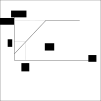
\includegraphics[width=\defaultwidth]{barral}
  \caption{Linear-saturated emission model from \citet{barral2003a}.}
  \label{fig-modelbarral}
\end{figure}

 We suppose that all of the electrons emitted are isotropically emitted following a Maxwellian flux distribution function of temperature $\Tsee$.
 The parameters $\proba_0$,  $\probamax$ and $\crover$ can be obtained from experiments. 
 \Cref{tab-seeparames} shows the crossover energy and the  probability of emission at energy null for different materials.
 The value of $\proba_0$ is always close to $0.5$, but $\crover$ can vary from 18 to 305 V.
 Hence, in the following parametric studies, $\proba_0$ will be kept at 0.5 while we vary $\crover$ from low values, corresponding to highly emmissive materials, to high values, representing less emmissive materials.
 
 \begin{table}[hbtp]
   \ra{1.3}
   \centering
   \caption{Emission parameters for different materials, from \citet{barral2003a}.}
   \label{tab-seeparames}
   \begin{tabular}{@{}lll@{}} \toprule
   Material & $\crover$ (V)& $\proba_0$ \\ \midrule
   BN-SiO$_2$ & 53 & 0.45 \\ 
   Al$_2$O$_3$ & 18  & 0.57 \\ 
   SiC     &  43  &0.69  \\
   Graphite & 305  & 0.40 \\ 
   \bottomrule
   \end{tabular}
 \end{table}
 

% !TEX root=/home/tavant/these/manuscript/src/manuscript.tex

\section{Electron cross-field transport}
  \label{sec-transport}
  
  The electron mobility in the axial direction $\mobe$ is defined as the ratio between the mean velocity $u$ and the electric field
  \begin{equation} \label{eq-mudef}
    \mobe = \frac{u_{e,z}}{E_z}
  \end{equation}
  with $u_{e,z}=<v_{e,z}>$ the electron mean velocity
  \nomenclature[Q]{\ensuremath{ u_{e,z}}}{Electron mean velocity int he axial direction : $u_{e,z} = < v_{e,z}>$}
  In the \ac{PIC} simulations, \cref{eq-mudef} can be used directed to compute $\mobpic$.
  
  In the classical drift diffusion theory of the electron mobility transverse to a magnetic field, the mobility is due to collisions as \citep{chen2006,meezan2001}
  \begin{equation} \label{eq-mobclas}
    \mobcla = \frac{e}{m_e} \frac{\nu_m}{\nu_m^2 + \oce^2}
  \end{equation}
  with $\oce=\frac{e B}{m_e}$ the electron cyclotron frequency and $\nu_m$ the electron-neutral momentum transfer collision frequency.
  \nomenclature[Q]{\ensuremath{ \oce}}{ Electron cyclotron frequency $\oce=\frac{e B}{m_e}$}
  \nomenclature[Q]{\ensuremath{ \nu_m}}{  electron-neutral momentum transfer collision frequency}
  
  At the exit plan, the classical mobility predict a mobility of the order of $\mobcla=0.001 -- 0.01\mobunit$ \citep{adam2008a}.
  
  The kinetic approach allowed \citet{lafleur2016a} to propose a modified mobility due to the oscillations of the electron density and the azimuthal electric field of the \ac{ECDI}.
  This effective mobility obtained is 
  \begin{equation} \label{eq-defmobeff}
    \mobeff = \mobcla \lp 1 - \frac{\oce}{\nu_m}  \frac{< \dne \dEt >_{\theta} }{n_0 E_z}   \rp
  \end{equation}
  with \dne and \dEt the fluctuations in the azimuthal directions of the electron density and azimuthal electric field, respectively, the operator $< . >_{\theta}$ is the average in the azimuthal direction, and $n_0$ is the average plasma density.
  In the case where $\nu_m << \oce$, \cref{eq-defmobeff} can be simplified to 
  \begin{align} 
    \mobeff &= \frac{\frac{e}{m_e} \nu_m}{\oce^2} \lp 1 - \frac{\oce^2}{\nu_m}  \frac{< \dne \dEt >_{\theta} }{n_0 E_z}   \rp \nonumber \\
    &= \frac{< \dne \dEt >_{\theta} }{n_0 E_z}   \frac{1}{B_r} \label{eq-mobeffsimple}
  \end{align}
  which shows that the instability enhances the electron axial mobility in a wave similar to an $E \times B$ drift.
  The electric field $E_{\theta}$ oscillates and presents a zero mean value, but the average effect on the electron transport is not zero if the correction between \dEt and \dne is not zero.
  
  In  \citet{lafleur2016a}, the authors present the instability effect as an electron-ion friction force $\Rei = - e < \dne \dEt >_{\theta}$.
  Under the assumption that the saturation of the instability is mainly due to ion trapping, the electron-ion friction force can be simplified to
  \begin{equation} \label{eq-rei-sat}
    \Rei^{sat} = \frac{e \norm{\grad \cdot (n_e \Te \vect{v_i})}}{4 \sqrt{6} c_s} \simeq \frac{e n_e \Te \viout}{4 \sqrt 6 c_s L_z}
  \end{equation} 
  \nomenclature[Q]{\ensuremath{ \vect{v_i}}}{  ion velocity vector}
  \nomenclature[Q]{\ensuremath{ c_s}}{ ion sound speed $c_s=(e \Te/m_i)^{1/2}$ }
  where $\vect{v_i}$ is the ion velocity, $c_s=(e \Te/m_i)^{1/2}$  is the ion sound speed, and the spatial derivative in has been approximated across the axial simulation direction, with $\viout$ the ion outlet velocity 
  \begin{equation} \label{eq-viz}
    \viout = \sqrt{\frac{2 e U_z}{m_i}},
  \end{equation}
  with $U_z = E_z L_z$ the total potential difference in the axial direction.
  \nomenclature[Q]{\ensuremath{ U_z}}{   total potential difference in the axial direction $U_z = E_z L_z$}
  
  Using \cref{eq-rei-sat} in \cref{eq-mobeffsimple}, we obtain the simplified expression
  \begin{equation} \label{eq-mobeffsat}
    \mobeffsat = \frac{\sqrt{\frac{\Te}{U_z}}}{4\sqrt{3}B_r}.
  \end{equation}
  
  \Cref{eq-mobeffsat} shows that for the radial and azimuthal \ac{2D} geometry being used here, the enhanced mobility due to \ac{ECDI} scales as the square-root of the electron temperature $\Te$ if the simulation parameters are constant.
  However, it is not the case in general, as the saturation of the instability can be also due to convection, and there are axial gradients in the electron temperature and plasma density as well.
  
  We can note that $\mobpic, \mobeff$ and $\mobcla$ are defined at every position of the simulation, but that $\mobeffsat$ can only be globally calculated. 
  
  
  
  
  
% !TEX root=/home/tavant/these/manuscript/src/manuscript.tex

\section{Sheath model with electron emission}
  \label{sec-sheath}
  
  \inlinenote{Ici, le model est introduit rapidement... Peut-etre le faire plus explicitement a partire des equations fluid ?}
  
  The sheath model featuring SEE processes has been historically studied by Hobbs and Wesson \citet{hobbs1967}, but is still an active research topic nowadays \citep{ahedo2005}.
  The sheath is often considered to be collision-less and isothermal, while the plasma is composed of hot Maxwellian electrons and cold ions. A third population of electron-induced secondary electrons is also present in the sheath, and the re-emission rate $\rate$ is assumed to be constant.
  The SEE process modifies the potential drop in the sheath as \citep{hobbs1967}
  \begin{equation} \label{eq-sheathhobbs}
    \dphisheath = \Tepar \ln \lp (1 - \rate) \sqrt{\frac{m_i}{2 \pi m_e}}   \rp
  \end{equation}
  with $\Tepar$ the electron temperature in the direction parallel to the magnetic field, thus normal to the walls.
  Adding a pre-sheath drop of $\Tepar/2$ \citep{ahedo2002}, the total potential drop to the wall becomes
  
  \begin{equation} \label{eq-total_drop}
    \dphi = \dphisheath + \frac{\Tepar}{2} =  \Tepar \lp \frac{1}{2} + \ln \lb (1 - \rate) \sqrt{\frac{m_i}{2 \pi m_e}}   \rb  \rp
  \end{equation}
  
  In \Cref{eq-sheathhobbs,eq-total_drop}, we uses $\Tepar$ as in general, and more precisely for low-pressure magnetized plasma, the electrons can be anisotrope.
  
  We can see that \cref{eq-sheathhobbs} becomes negative for a critical value of the emission rate
  \begin{equation} \label{eq-ratecrone}
    \rate_{\rm max} = 1 - \sqrt{\frac{2 \pi m_e}{m_i}} \simeq 0.985 \text{ for Xenon.}
  \end{equation}
  
  However, before that $\rate$ attains $\rate_{\rm max}$, the model of \citet{hobbs1967} presents another behaviour against the hypotheses of  \cref{eq-sheathhobbs}, as the sheath becomes \ac{SCL}.
  In the \ac{SCL} conditions, the electron emission is so large that the electric field at the wall becomes zero 
  \begin{equation} \label{eq-scl_Er}
    \deriv{\phi}{r} \at{\rm wall}= 0 
  \end{equation}
  In this case, the plasma potential drop to the wall for any ion mass is \citep{hobbs1967}
  \begin{equation} \label{eq-dphi_scl}
    \dphiscl \simeq 1.02 \Tepar,
  \end{equation}
  and the limit emission rate is
  \begin{equation} \label{eq-ratecr}
    \ratecr \simeq 1 - 8.3 \sqrt{\frac{m_e}{m_i}}
  \end{equation}

  For xenon, \cref{eq-ratecr} gives $\ratecr = 0.983$ \citep{goebel2008}.\footnote{This value of 0.983 is obtained after several approximation, as \cref{eq-scl_Er} , some of which should not allow to use three significant digits. That's why it does not exactly match with the numerical results presented in \cref{fig-potential_profile}.}

  \Cref{fig-potential_profile} illustrates the sheath model of \citet{hobbs1967} by showing the plasma potential profile in the sheath for different values of electron emission rate for a xenon plasma.
  \cref{fig-potential_profile}.{\bf a} gives the potential $\phi$ normalized by $\dphisheath$ from \cref{eq-sheathhobbs}, and \cref{fig-potential_profile}.{\bf b} gives $\phi$ not normalized.
  We can see in \cref{fig-potential_profile}  that for $\rate < \ratecr$, the plasma potential reached $\dphisheath$.
  However, for $\rate > \ratecr$, the plasma potential do not reaches $\dphisheath$, resulting in a non-zero current to the wall.
  Indeed, the sheath is not monotonic in this case, hence the hypotheses needed to develop \cref{eq-sheathhobbs} are not fulfilled.
  
  In \cref{fig-potential_profile}.{\bf b}, we can see that at $\rate \simeq \ratecr$, the plasma potential tends towards $\Te$, as mentioned by \cref{eq-dphi_scl}.
  \begin{figure}[hbtp]
    \centering
    \begin{tabular}{c c}
      \subfigure{plasma_profile_normed}{a}{25,20} & 
      \subfigure{plasma_profile}{b}{25,20} 
    \end{tabular}
    \caption{Evolution of the plasma potential in the sheath for different values of electron emission rate $\rate$ fro a xenon plasma, ({\bf a}) normalized by the total potential drop $\dphisheath$ from \cref{eq-sheathhobbs}, and ({\bf b}) normalized by the electron temperature, but $\dphisheath/\Te$ is noted with the black dotted line.  }
    \label{fig-potential_profile}
  \end{figure}
  
  
% !TEX root=/home/tavant/these/manuscript/src/manuscript.tex



\section{Conclusion}
  \label{sec-conclusion_ch1}
  

  In order to study the plasma wall interaction in an \ac{HET}, we developed a bi-dimensional simulation code using \ac{PIC}-\ac{MCC} modeling.
  As the electrons drift azimuthally due to the $E \times B$ configuration, the \ac{ECDI} rises, enhancing the cross field transport of the electron toward the anode.
  The walls closing the chamber in the radial direction are also important for the discharge behaviour.
  Hence, in order to compare the interaction between these phenomena, we simulate the radial-azimuthal domain.
  
  A special care have been taken during the developement of \LPPic, the \ac{2D}-\ac{3V} \ac{PIC}-\ac{MCC} simulation code, concerning
  \begin{itemize}
    \item the modeling of the axial convection, in order to model the energy losses and so attain a steady state,
    \item the modeling of the radial boundary with the dielectric layer included in the simulation domain.
  \end{itemize}
  
  Several theories have also been given in order to better understand the \ac{PIC} simulation results, especially concerning the electron cross-field mobility and the sheath model in presence of electron emission.

% \acresetall
% !TEX root=/home/tavant/these/manuscript/src/manuscript.tex




\chapter{Parametric study of the dielectric characteristics}
\label{ch-2}
\headerchaptername{Dielectric parametric study}

\begin{Chabstract}
We use the PIC simulation code described in \cref{ch-1} to perform a parametric study over the two aspects of the dielectric walls\string: the secondary electron emission, and the modification of the electrostatic boundary condition.
We observe their impacts on the electron cross-field mobility, the electron mean temperature and the sheath characteristics.
The electrostatic boundary condition does not modify the results significantly.
On the other hand, the electron emission increases the near-wall mobility while decreasing the mean electron temperature, that reduces the importance of the \ac{ECDI} on the mobility.
A large discrepancy is observed between the sheath model of \cref{sec-sheath} and the PIC simulation results.
\end{Chabstract}



\minitoc


% 
% Structure \string:
% 
% {\bf II. Parametric study of the dielectric} 30 pages
% \begin{zzz}
%   This chapter takes the 1rst paper which uses Vivien's results.
% 
%   2.1 Fully metallic wall (no SEE, grounded).
% 
%   2.2 Impact of Dielectric layer without SEE
% 
%   2.3 Impact of SEE with grounded wall
% 
%   2.4 SEE and dielectric in the same time
% 
%   2.5 Discrepancy between $\mean{\Te}$, $\sigma_{PIC}$ and $\sigma_{theo} = \sigma_0 + (1 - \sigma_0) \frac{2 T_e}{\epsilon_0}$
% \end{zzz}


% !TEX root=/home/tavant/these/manuscript/src/manuscript.tex

\section{Simulation parameters}
  \label{sec-params}
  
  The simulation domain corresponds to the exit plane of the thruster.
  Hence, a neutral pressure $P_n$ of 0.1~mTorr and a plasma density $n_e$ of $\sn{1}{17}$ m$^{-3}$ are used.
  The fixed axial electric field and radial magnetic field are $E_z=\sn{2}{4}\,\volt\per\meter$ s and $B_r=200$ G, respectively.
  The rectangular \ac{2D} domain measures $L_r=2$~cm in the radial dimension and $L_{\theta}=0.5$~cm in the azimuthal direction.
  The axial length used for the convection is fixed at $L_z=1$~cm.
  It is important to note that the results shown in this chapter have been obtained at the beginning of my thesis, before the study of the convection presented in \cref{ch-1}.
  Hence, in this chapter we use the convection model of \citet{lafleur2016a}.
  However, we have validated at posteriori that the convection model used does not modify the results under the conditions studied.
  
  The numerical parameters are chosen to respect the stability criterion of \ac{PIC} simulation, and are presented in \Cref{parameters}
  
  \begin{table}[htbp] %PIC parameters
       \centering
       \ra{1.3}
       \caption{\label{parameters} Standard operating and numerical parameters used in the 2D PIC simulations of an HET.  The simulation results are given as representative values.}
       \begin{tabular}{@{}r c c c@{}} 
          \toprule
          {\bf Physical Parameter} & notation & Value & Unit \\
          \midrule
          Gas & & Xenon & - \\
          Domain dimensions & $L_{x} \times L_{y} \times L_{z}$ & $2.0 \times 0.5 \times 1.0$ & [cm$^3$] \\
          Radial magnetic field & $B_{0}$                    & $200$                 & [{G}] \\
          Axial electric field & $E_{0}$                    & $2 \times 10^{4}$     & [{Vm}$^{-1}$] \\
          Mean plasma density & $n_{0}$                    & $3 \times 10^{17}$    & [{m}$^{-3}$] \\
          Initial electron temperature & $\Te_{,0}  $               & $5.0$                 & [{V}] \\
          Initial ion temperature & $T_{i,0}   $               & $0.1$                 & [{V}] \\
          Secondary electron temperature & $T_{see}   $               & $1.0$                 & [{V}] \\
          Neutral gas pressure & $P_{n}     $               & $1.0$                 & [{mTorr}] \\
          Neutral gas temperature & $T_{n}     $               & $300$                 & [{K}] \\
          Neutral gas density & $n_{g}     $               & $3.22 \times 10^{19}$ & [{m}$^{-3}$]\\
          \midrule
          {\bf Simulation Parameter} &  &   &  \\
          
          Time step & $\Delta t  $                      & $4 \times 10^{-12}$ & [{s}] \\
          Cell size & $\Delta x = \Delta y = \Delta z $ & $2 \times 10^{-5}$  & [{m}] \\
          Number of particles per cell & $N/NG      $                      & $80$                & [{part/cell}] \\
          \midrule
          {\bf Typical quantities} &  &  &  \\ 
          Electron plasma frequency & $\omega_{pe}$               & $3.1 \times 10^{10} $  & [rad/s]\\
          Iopn plasma frequency & $\omega_{pi}$               & $36 \times 10^{6} $  & [rad/s]\\
          Electron cyclotron frequency & $\omega_{ce}$               &  $3.5\times 10^{9}$  & [rad/s] \\
          Electron Larmor radius & $r_{Le}$                    & 6$\times 10^{-4}$    & [m] \\
          \bottomrule
       \end{tabular}
    \end{table}
  
  
  The simulation is initialized with a uniform density of particles, following a Maxwellian distribution for temperature $\Te_{,0}$ and $\Ti_{,0}$ for the electrons and the ions respectively.
  
  
% !TEX root=/home/tavant/these/manuscript/src/manuscript.tex

\section{The base case}
  \label{sec-canonical}
  
  
  The {\it base} case corresponds to the case when the walls are grounded, and are fully absorbing. 
  It is the reference case that will be extensively described and commented.
  Then, it will be used as reference to analyze and quantify the effects of two characteristics of the dielectric walls on the studied discharges : the secondary electron emission, and the modification of the electrostatic boundary condition.
  
  \subsection{Initial phase of the simulation\string: \texorpdfstring{$t < 2\,\micro\second$}{ t < 2 microseconds} } \label{subsec-initlaphase}
  
  The initial phase of the simulation corresponds to the growth of the \ac{ECDI}, and the formation of the sheaths.
  Because of the growth of the instability, the electron transport increases as well, which increases the electron heating.
  The time scale of the sheath formation is governed by the ion inertia.
  It is roughly the same time scale as the saturation of the instability due to ion-trapping.
  
  \begin{figure}[hbt]
    \centering
    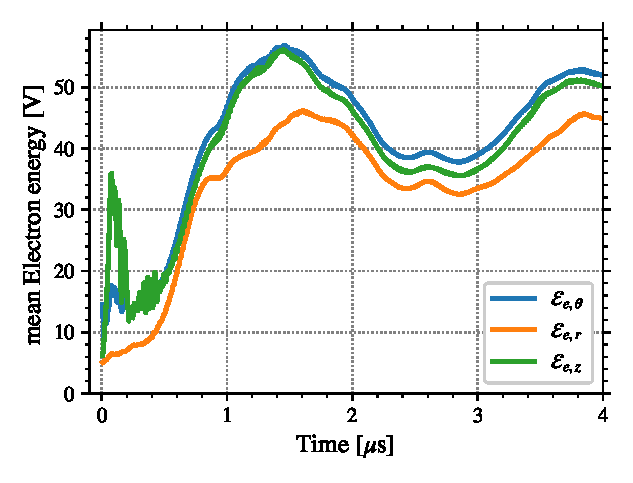
\includegraphics[width=\defaultwidth]{canonical_Te_start_directions}
    \caption{Temporal evolution of the electron mean kinetic energy decomposed over the three directions. Only the beginning of the simulation is shown.}
    \label{fig-canon_Te_strat}
  \end{figure}
  
  \Cref{fig-canon_Te_strat} shows the temporal evolution of the electron mean kinetic energy decomposed over the three directions, $\Ee_r, \Ee_{\theta}, \Ee_z$, such that
  \begin{equation} \label{eq-Ee_direction}
    \Ee_d = \frac{1}{n} \frac{1}{2} m_e \iiint_{\vect{v}}  v_{e,d}^2 f (\vect{v}) d^3v, \text{ with } d \in \{r, \theta, z  \}
  \end{equation}
  The mean kinetic energy is the sum of the thermal energy and the kinetic energy of the mean velocity.
  Because the electrons drift mainly in the azimuthal direction, we have
  \begin{equation} \label{eq-kinetic}
    \begin{cases}
      \Ee_r \simeq \frac{\Te_r}{2} \\
      \Ee_z \simeq \frac{\Te_z}{2} \\
      \Ee_{\theta} \simeq \frac{\Te_{\theta}}{2} + \frac{m_e}{2} \lp \frac{E_0}{B_0} \rp^2 \\
    \end{cases}
  \end{equation} 
  with $\frac{m_e}{2} \lp \frac{E_0}{B_0} \rp^2 \simeq  2.84\,\volt $.
  \nomenclature[Q]{\ensuremath{ \Ee}}{ Electron total kinetic energy, imposed of the thermal (or internal) energy and the kinetic energy of the mean velocity.  }
  We see that after some high frequency oscillations of $\Ee_{\theta}$ and $\Ee_z$ due to the cyclotron motion, the energies rise before stabilizing at $\Ee \simeq 45$V.
  The radial kinetic energy $\Ee_r$ is less than $\Ee_z$ and $\Ee_{\theta}$, but only by a small difference of $5\,\volt$, corresponding to roughly $10\%$.
  The small difference between the azimuthal and the axial kinetic energy is of the order of $2\,\volt$, as expected from the cyclotron motion of the electrons and \cref{eq-kinetic}.
  This means that the electrons are almost isotropic.
  
  
  \begin{figure}[hbt]
    \centering
    \begin{tabular}{@{} c c}
      \subfigure{time_r_mean_n}{a}{20, 20} &
          
      \subfigure{time_r_mean_phi}{b}{20, 20} 
    \end{tabular}
    \caption{Temporal evolution of the radial profile of the ({\bf a}) electron density and ({\bf b}) the plasma potential averaged azimuthally.}
    \label{fig-tx_n_phi}
  \end{figure}

  We can see in \Cref{fig-tx_n_phi} the evolution of the radial profile of the electron density on the plasma potential over the same period as \cref{fig-canon_Te_strat}.
  We observe on both quantities the formation of the sheath and the evolution toward a steady-state.
  
  \subsection{Saturated quasi steady-state\string: \texorpdfstring{$t \geq 2\,\micro\second$}{t > 2 microseconds}  }
  \label{subsec-stablephase}
  After the relatively fast rise of the plasma characteristics, the simulation reaches a quasi steady-state, as we can see in \Cref{fig-canon_Te_all}.
  We observe that after $t\simeq2\mus$ , the electron energy $\Ee$ starts to oscillate around a mean value.
  The oscillations are then damped and reach their minimum amplitude at  $t\simeq 7\mus$ and then remain with a small amplitude as shown on simulations carried out up to $25\,\micro\second$ in \cref{fig-canon_Te_all} (the origin of these oscillations has been discussed in \Cref{subsec-temp}).  
  
  
  \begin{figure}[hbt]
    \centering
    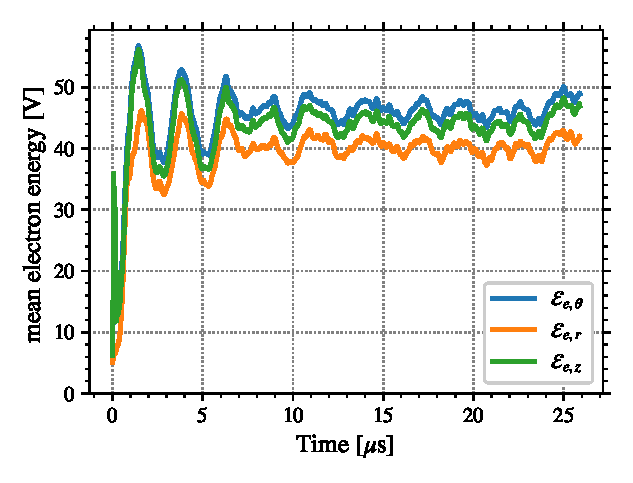
\includegraphics[width=\defaultwidth]{canonical_Te_all_directions_long}
    \caption{Temporal evolution of the electron mean kinetic energy decomposed over the three directions, similar to \cref{fig-canon_Te_strat} but for a longer period. We still see the difference between $\Ee_z$ and $\Ee_{\theta}$ due to the $E\times B$ drift, and the colder radial energy.}
    \label{fig-canon_Te_all}
  \end{figure}
  

  \Cref{fig-profiles} shows the azimuthally-averaged radial profiles of the electron and ion densities.
  The plasma is mostly quasineutral, except close to the walls, in the sheath, where the electron density falls more rapidly compared to that of ions.
  The sheath length can be roughly estimated to be $1\,\milli\meter$.
  The Debye length in our conditions is
  \begin{equation} \label{eq-debye}
    \lambda_D = \sqrt{\frac{\epsilon_0 k_b T_e}{n_e e^2}} \sim 0.4\,\milli\meter,
  \end{equation}
  which corresponds to the expected floating sheath length \citep{chabert2014} (a few $\lde$).
  
  \begin{figure}[hbt]
    \centering
    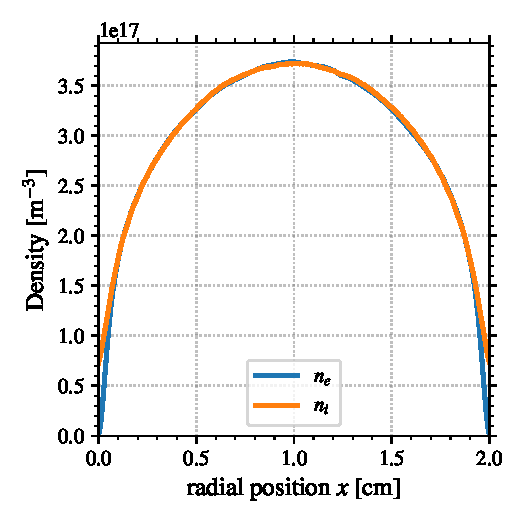
\includegraphics[width=\defaultwidth]{density_profile.pdf}
    \caption{Radial profile of the ion and electron densities at steady-state, averaged azimuthally and in time over the 5 last microseconds.}
    \label{fig-profiles}
  \end{figure}
  
  \subsection{Enhanced electron transport} \label{subsec-canonmue}
  As introduced in \cref{sec-transport}, the electron cross-field axial transport is characterized by the electron mobility
  \begin{equation} \label{eq-mobdef}
    \mob = \frac{u_{e, z}}{E_z}
  \end{equation}
  with $u_{e,z}$ and $E_z$ the electron mean axial velocity and the axial electric field, respectively.
  \nomenclature[Q]{\ensuremath{ \mob}}{ Electron mobility}
  \nomenclature[Q]{\ensuremath{ u}}{ Electron mean velocity}
  In \ac{PIC} simulations, $\mob$ is computed at each time step by
  \begin{equation} \label{eq-mobpic}
    \mobpic = \frac{1}{N E_z} \sum_N v_{e,z}
  \end{equation}

  \begin{figure}[hbt]
    \centering
    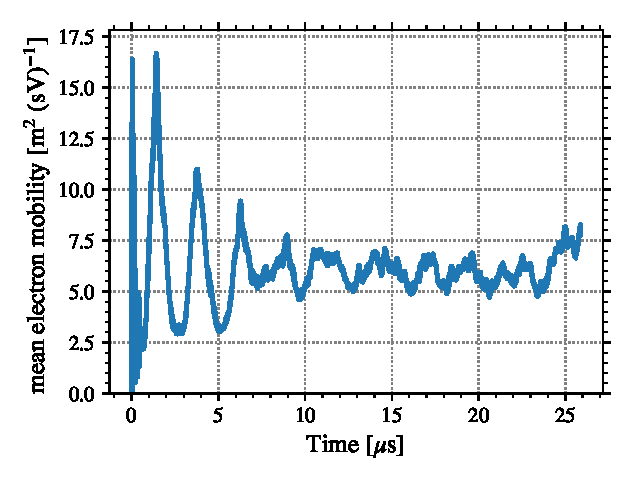
\includegraphics[width=\defaultwidth]{canonical_mu_all}
    \caption{Temporal evolution of the electron axial mobility computed in the \acs{PIC} simulation.}
    \label{fig-canon_mu}
  \end{figure}
  
  \Cref{fig-canon_mu} shows the temporal evolution of the electron mobility $\mobpic$ measured in the simulation with \cref{eq-mobpic}.
  We can see that it presents the same characteristics as the evolution of the electron energy $\Ee$ on \cref{fig-canon_Te_all}.
  We recall that the classical electron mobility from the collisional theory developed in \cref{eq-mobility} is \citep{lafleur2016a}
  \begin{equation} \label{eq-muclass}
    \mobcla = \frac{\nu_m \frac{e}{m_e}}{\oce^2 + \nu_m^2}
  \end{equation}
  with $\nu_m$ the electron-neutral  collision frequency and \oce{} is the electron cyclotron frequency.
  In the conditions of \cref{parameters}, $\mobcla \simeq 0.8$ \square\meter(sV)$^{-1}$.
  
  The measured electron mobility in the \ac{PIC} simulation is one order of magnitude larger than the classical mobility.
  In the present case, as no electron is emitted from the wall, the enhancement can only come from the instabilities present in the plasma.

  % K_ex = 2 10^-13
  % n_g = 1e19
  % wce = q B / m
  The oscillations can be seen in \cref{fig-2dschemat}, which shows the azimuthal electric field observed at $T=4\,\micro\second$.
  It clearly features the oscillation of wavelength of the order of 1~mm, as observed in \citet{heron2013}, and \citet{janhunen2018}.
  \Cref{fig-exampleECDI} shows the temporal evolution of the azimuthal electric field measured at the center of the channel.
  We can see that the instability rises and saturates quickly.
  Then, the oscillation remains quite stable.
  The Fourier Transform of the electric field presents a clear maximum at $14\,\mega\hertz$.
  The theoretical frequency of the \ac{ECDI} instability is \citep{lafleur2017}
  \begin{equation} \label{eq-maxfeq}
    f_{\rm max} = \frac{\omega_{pi}}{\sqrt{3}} \simeq 21 \,\mega\hertz,
  \end{equation}
  which gives a relatively good agreement with the oscillation observed.
  The \ac{ECDI} instability was the subject of \Cref{ch-5}, hence it will not be further discussed here.
  
  
  \begin{figure}[hbt]
    \centering
    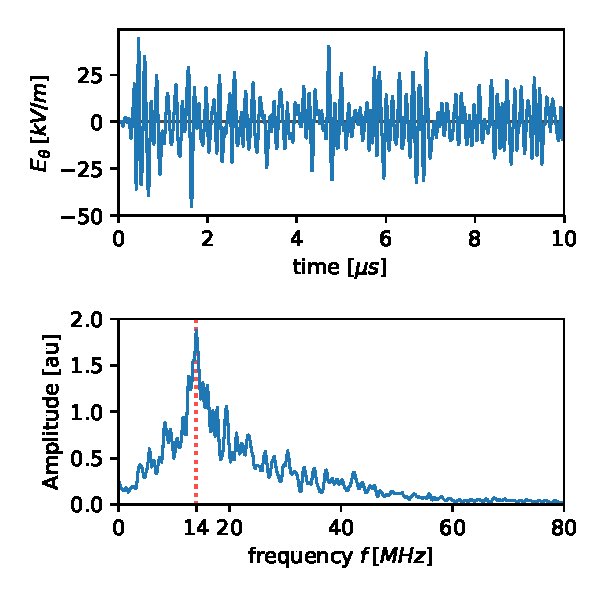
\includegraphics[width=\defaultwidth]{time_and_FFT}
    \caption{Azimuthal instability\string: temporal evolution of the azimuthal electric field at the center of the simulations, and its frequency spectrum computed by \acs{FFT}. The frequency for which the amplitude is maximum is highlighted.}
    \label{fig-exampleECDI}
  \end{figure}
  
  The effective mobility $\mobeff$ is determined by the correlation term $<\dEt \dne>$ and the parameters of the simulations.
  The effective mobility at saturation $\mobeffsat$, using the hypothesis of saturation by ion-wave trapping, only needs the electron temperature $\Te$.
  We can see that the three values $\mobpic, \mobeff$, and $\mobeffsat$ are close from each-others.
  
  \begin{table}[!hbt]
  \ra{1.3}
    \centering
    \caption{Characteristics  measured in the simulation at $t=27\,\micro\second$.}
    \label{tab-canonical_mobility}
    \begin{tabular}{@{} r l @{}} \toprule
    Quantity & Value \\ \midrule
    Correlation $<\dEt \dne>$ & $\sn{6}{20}$ V/m${^4}$ \\
    Effective mobility $\mobeff$ from \cref{eq-eq_mobeffsimple_two} & 4.4 m$^2$(sV)$^{-1}$ \\
    Mobility saturation $\mobeffsat$ from \cref{eq-mobeffsat} & 3.3 m$^2$(sV)$^{-1}$ \\
    Measured mobility $\mobpic$ from \cref{eq-mobpic} & 6 m$^2$(sV)$^{-1}$\\
    \bottomrule
    \end{tabular}
  \end{table}
  

  
  
% !TEX root=/home/tavant/these/manuscript/src/manuscript.tex

\section{Modeling the dielectric layer }
  \label{sec-diel_layer}
  
  The first effect of the wall material studied is adding a layer of dielectric material with its own permittivity, as introduced in \Cref{sec-diel}.
  The simulation parameters are the same as in the canonical case, presented in \cref{sec-canonical}, but the plasma is separated from the ground wall by a dielectric layer of 3~mm.
  Hence, the distance between the grounded electrodes is $2.6\,\centi\meter$.
  The relative permittivity of the dielectric is $\epsr=25$.
  %% SEE runs 250et 257 ?? Ly=1cm, Diel avec et sans SEE
  
  \Cref{fig-diel_radial_Er} shows the radial profile of the radial electric field $E_R$ at $t=10\,\micro\second$ averaged in the azimuthal direction.
  The plasma domain starts at $r=0$ and finishes at $r=2\,\centi\meter$.
  We note the jump in the value of the electric field at the plasma-wall transition.
  This jump is due to the surface charge.
  We can also notice that in the dielectric layer, in $r < 0$ and $r > 2\,\centi\meter$, the radial electric field is close to zero, compared to the value in the sheath.
  
  \begin{figure}[hbt]
    \centering
    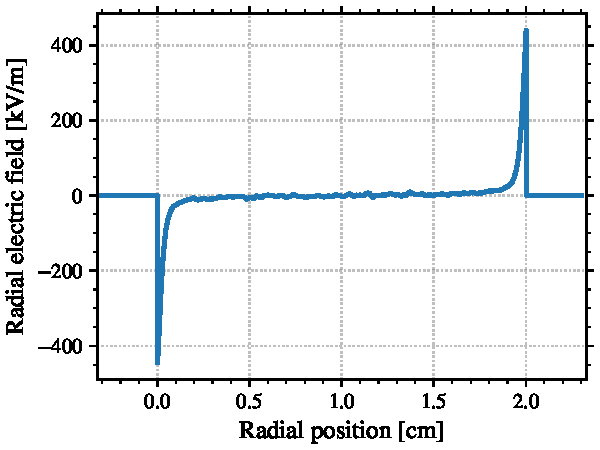
\includegraphics[width=\defaultwidth]{diel_average_radial_electric_field}
    \caption{Radial profile of the radial electric field $E_R$ averaged in the azimuthal direction at $t=10\,\micro\second$. The plasma domain starts at $r=0$ and finishes at $r=2\,\centi\meter$. The dielectric length is $L_{\\rm Diel} = 3\,\milli\meter$.  }
    \label{fig-diel_radial_Er}
  \end{figure}
  
  The next sections investigate the impact of the dielectric layer on the plasma characteristics, and highlight the plasma-wall interaction.
  
  \subsection{Effect of the dielectric layer} \label{subsec-effect_mob}
    
  
  The simulation results are qualitatively the same as in the case without the dielectric layer.
  As an example, \Cref{fig-mod_diel_comp} shows the temporal evolution of the axial electron mobility with and without the dielectric layer.
  We see that the results for the electron temperature and mobility are similar.
  The low amplitude oscillation of the case with the dielectric decreases slightly slower.
  
  \begin{figure}[hbt]
    \centering
    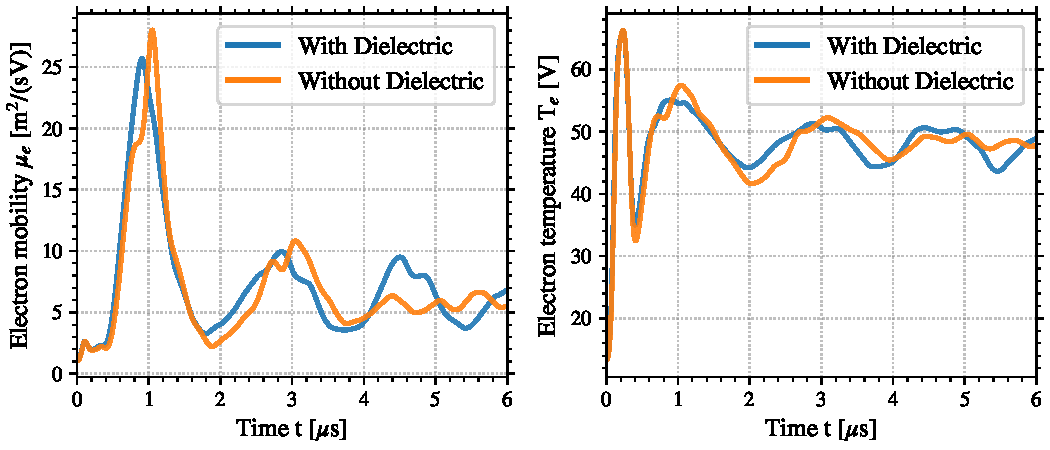
\includegraphics[width=\textwidth]{Dielectric_noSEE_temporal.pdf}
    \caption{Temporal evolution of the axial electron mobility (left), and the electron temperature (right) with and without the dielectric layer modeled.}
    \label{fig-mod_diel_comp}
  \end{figure}

  
  \subsection{Near-wall and in-wall parameters} \label{subsec-nearwall}
    In this section, we focus on the surface charge and the near-wall electric field.
    \Cref{fig-sigma_time} shows the temporal evolution of the surface charge at one point of the wall.
    The position has been chosen to be the center ($L_{\theta} = 0.25$~cm) of the lower wall, but the observations are similar at other positions.
     
    \begin{figure}[hbt]
      \centering
      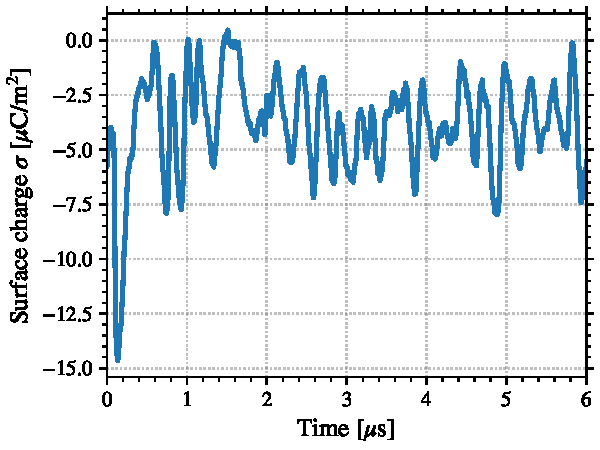
\includegraphics[width=\defaultwidth]{temporal_sigma}
      \caption{Temporal evolution of the surface charge $\sigma$ at one position of the lower dielectric wall}
      \label{fig-sigma_time}
    \end{figure}

    We can see on \cref{fig-sigma_time} that the value of the surface charge start by decreasing significantly (increasing in absolute value), due to the hot electrons that reach quickly the walls.
    Then, $\sigma$ growth and oscillates around a mean value close to $-3.5 \,\micro\coulomb/\square\meter$ and with an amplitude of approximately $1.2 \,\micro\coulomb/\square\meter$.
    
    \cref{fig-indiel} shows the azimuthal evolution of the radial electric field inside the dielectric layer.
    The electric field is given at three different positions ($r=-0.2, -0.9,$ and $-1.8\,\milli\meter$ away from the plasma-wall interface) to highlight its evolution.
    We can see that, even thought there is no charge in the dielectric, the amplitude of the electric field decreases when going further away from the plasma.
    This is due to the \ac{2D} Poisson equation, which smooth-out the inhomogeneity.
     
    \begin{figure}[hbt]
      \centering
      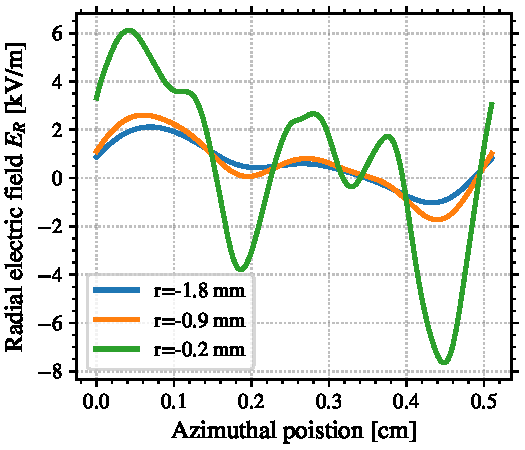
\includegraphics[width=\defaultwidth]{Radial_electric_feld_in_diel.pdf}
      \caption{Azimuthal evolution of the radial electric field inside of the dielectric layer at three different positions; the reference $r=0$ is the plasma-wall interface, the grounded electrode is located at $r=-3\,\milli\meter$.}
      \label{fig-indiel}
    \end{figure}

    
  \subsection{Dielectric model comparison} \label{subsec-modelcomp}
  
  \inlinenote{Anne: {\bf Beaucoup de remarques sur cette partie: pas assez claire, décrire plus les valeures observées, etc. Voir les notes sur le pdf (22 juillet)}}
  
  As introduced in \cref{sec-diel}, a simplified approach to model the effect of the surface charges on the plasma is to use a Neumann boundary condition \citep{taccogna2019}
  \begin{equation} \label{eq-neuman}
    E_r = \frac{\sigma}{\epsilon_0}.
  \end{equation}
  \Cref{eq-neuman} uses two approximations\string:
  \begin{itemize}
    \item one dimensional
    \item No electric field in the dielectric
  \end{itemize}
  We have already seen in \cref{fig-indiel} that the electric field in the dielectric is not zero, but instead it oscillates in respect to the azimuthal instability present in the plasma.  
  \Cref{fig-spacial_comparaison} shows the radial electric field at the wall and compares it to would be obtained by \cref{eq-neuman}.
  We can see that the two values are of the same order of magnitude, close to $-500$~kV/m.
  However, the two values are not equal, as they oscillates around their mean value.
  We can see that the surface charge oscillates more than the actual electric field obtained by solving the Poisson equation.

\begin{figure}[hbt]
  \centering
  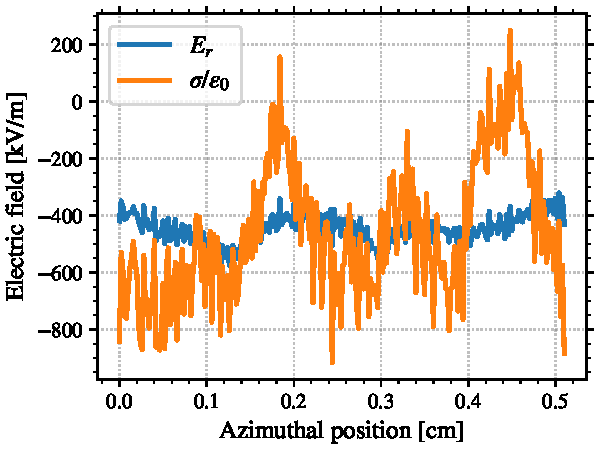
\includegraphics[width=\defaultwidth]{Radila_electric_field.pdf}
  \caption{Azimuthal evolution of the radial electric field at the plasma-wall interface and the electric field that would result from surface charge according to \cref{eq-neuman}.}
  \label{fig-spacial_comparaison}
\end{figure}
\renewcommand\subfigurewidth{0.45\textwidth}

  As a conclusion, we have observed that the dielectric layer does not change the simulation results much, but it can modify the surface processes.
  The model use here for the dielectric layer does not modify the performance of the simulation, while allowing to take into account the \ac{2D} effects.
  In this section, no secondary electron emission has been taken into account.
  In \cref{sec-fulldiel}, we will discuss the influence of using the simplified \cref{eq-neuman} in the case where secondary electron emission is important.

  
% !TEX root=/home/tavant/these/manuscript/src/manuscript.tex

\section{Impact of the radial boundary conditions on the oscillation}
  \label{subsec-BC}

  In \Cref{sec-DR-BC}, we discussed the choice of the radial wavenumber of the instability observed.
  Changing the radial electric boundary condition could affect the instability.
  Therefore, we discuss in this section  the impacts of the dielectric electrostatic boundary condition on the oscillation.
  We have seen in \Cref{sec-diel_layer} that the dielectric boundary did not affect the simulation results macroscopic.
  \Cref{fig-closswallosci} shows the radial evolution in the first few cells of the amplitude of the oscillation of the azimuthal electric field on the left, and the ion density on the right, with grounded (metallic) wall and dielectric wall.
  
  \begin{figure}[!hbt]
    \centering
    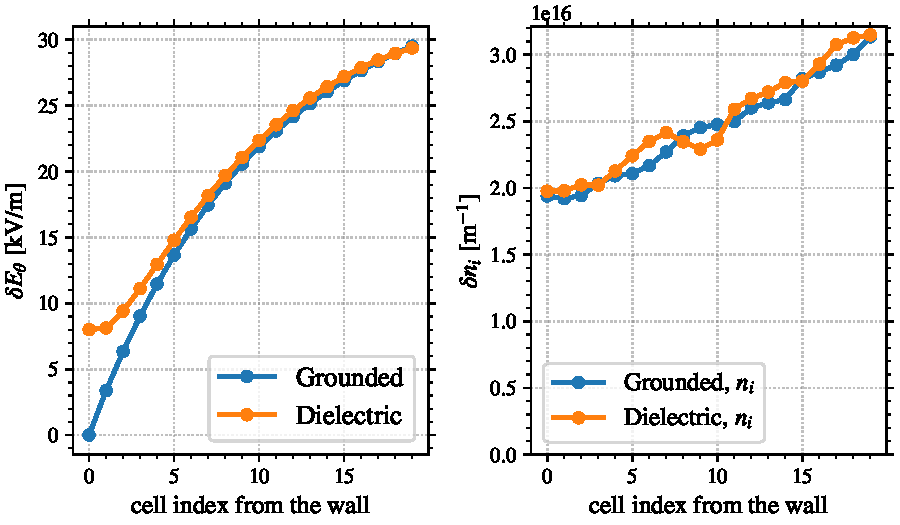
\includegraphics[width=\textwidth]{Ex_closewall.pdf}
    \caption{Radial evolution in the first cells of the amplitude of the oscillation of (left) the azimuthal electric field and (right) the ion density, with grounded (metallic) wall and dielectric wall.}
    \label{fig-closswallosci}
  \end{figure}
  
  We can see in \cref{fig-closswallosci} that the boundary condition does not affects the ion oscillations.
  This is consistent with the observation in \cref{subsec-kr} that the ion fluctuation was not affected by the wall.
  On the other hand, the azimuthal electric field has to go to zero when the wall is grounded.
  In contrast, using the dielectric boundary condition, the azimuthal electric field at the wall limit can be more than zero.
  Indeed, as seen in \cref{fig-indiel}, the amplitude of the azimuthal electric field decreases toward zero inside of the dielectric layer.
  
  Nevertheless, the difference in $E_{\theta}$ between the two boundary conditions quickly disappears inside the plasma domain.
  Indeed, after a dozen cells, corresponding to a few Debye lengths, the amplitudes of $\delta E_{\theta}$ are equal for both cases.
  Hence, the electrostatic boundary condition induces only minor differences in the instability and therefore the plasma discharge.
  
  
% !TEX root=/home/tavant/these/manuscript/src/manuscript.tex

\section{Effect of electron emission}
  \label{sec-see}
  
  In \Cref{sec-canonical}, the walls are not emissive.
  However, the dielectric ceramic used in \ac{HET} can emit electrons \citep{villemant2018,barral2003a}.
  The electron emission model used, introduced in \cref{sec-modelused}, has three parameters $\proba_0, \crover, \probamax$, such that the emission probability depends on the kinetic energy of the incident electron $\ek$ as
  \begin{equation} \label{eq-barral_second}
    \proba = \min \lp \proba_0 + (1 -  \proba_0) \frac{\ek}{\crover}, \probamax    \rp.
  \end{equation}
  
  The value of parameters are summarized in \cref{tab-tabe_parameters_see}.
  The crossover energy $\crover$ is varied from as low as 4~V, corresponding to a very emissive material, to as high as 200~V, a less emissive material.
  
  \begin{table}[hbtp]
  \ra{1.3}
    \centering
    \caption{Parameters of the electron emission probability model}
    \label{tab-tabe_parameters_see}
    \begin{tabular}{@{}ll@{}} \toprule
    Parameter & value  \\ \midrule
    $\proba_0$ & 0.5  \\
    $\probamax$ & 2.9 \\
    $\crover$   &  4  -- 200 V\\
    \bottomrule
    \end{tabular}
  \end{table}
  
  \begin{figure}[hbtp]
    \centering
    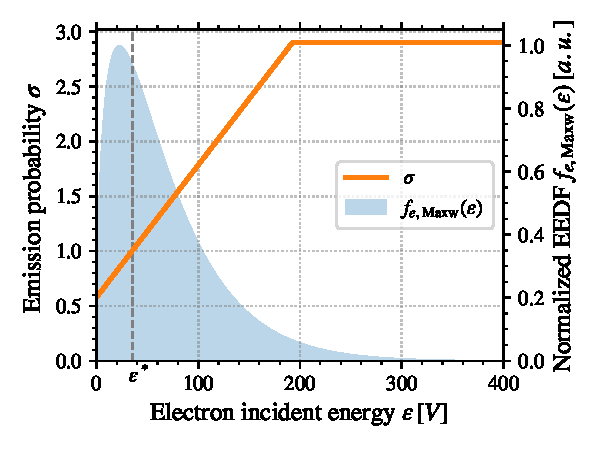
\includegraphics[width=\defaultwidth]{SEE_models}
    \caption{Illustration of the electron emission model of \cref{eq-barral_second} compared to a Maxwellian energy distribution function of temperature of 45~V, with $\crover=35.04$~V.}
    \label{fig-see_illustration}
  \end{figure}
  
  \Cref{fig-see_illustration} shows the electron emission probability for $\crover=35.04$~V compared to a Maxwellian \ac{EEDF} of temperature of 45~V.
  We can see that the saturation of $\proba$ at $\probamax$ happens only for the very high energy tail.
  In the simulation, we can only measure the average electron emission yield, also named emission rate, 
  \begin{equation} \label{eq-seeyield}
    \rate = \frac{\Gamma_{\rm emitted}}{\Gamma_{\rm incident}} = \frac{\iiint v_r \proba(\vect{v}) f(\vect{v}) d^3v}{\iiint v_r  f(\vect{v}) d^3v}.
  \end{equation}
  In general, \cref{eq-seeyield} cannot be calculated analytically.
  However, if we suppose that the \ac{EEDF} is Maxwellian and neglect the saturation at $\probamax$, \cref{eq-seeyield} yields
  \begin{equation} \label{eq-seemaxw}
    \ratemaxw(\Te) = \proba_0 + (1 - \proba_0) \frac{2 \Te}{\crover}.
  \end{equation}
  The saturation at $\probamax$ can be neglected as we have seen that it only affects a small part of the electron population, see \cref{fig-see_illustration}.
  \inlinenote{Add the exact calculation and the relative error ? \\Anne: oui. si trop long, a mettre en annexe.}
  
  \subsection{Impact of the electron emission of the mobility} \label{subsec-param-mob}
    
  The effects of the electron emission at the wall on the electron axial mobility are presented in \Cref{fig-mob-epsstar}.
  The measured mobility $\mobpic$ are shown, as well as the effective mobility $\mobeff$, the saturation estimate $\mobeffsat$ and the classical mobility $\mobcla$, defined in \cref{sec-transport} respectively by \cref{eq-mudef}, \cref{eq-defmobeff}, \cref{eq-mobeffsat} and \cref{eq-mobclas}.
  The values are averaged in time between $t=5 \mus$ and $t=10\mus$, and in space over the azimuthal and radial directions.
  \inlinenote{Anne: For epsilon=0, we have the values presented in section 2.2 without dielectrics.}
  \begin{figure}[hbtp]
    \centering
    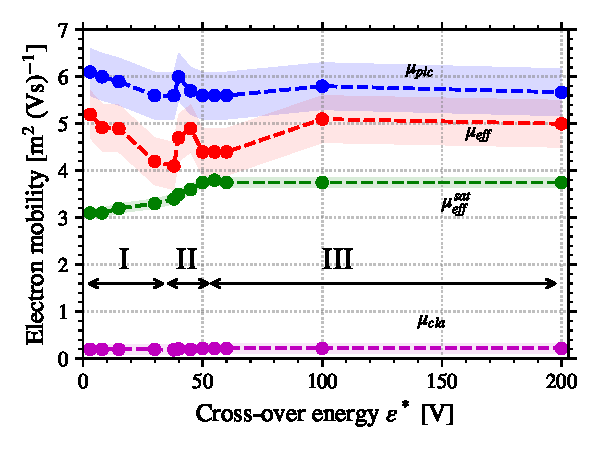
\includegraphics[width=\defaultwidth]{parametric_mobs_eps_complete}
    \caption{Evolution of the electron mobility as a function of the crossover energy $\crover$. In blue $\mobpic$ is the mobility measured in the simulations, while $\mobcla, \mobeff$ and $\mobeffsat$ in purple, red and green respectively are calculated with \cref{eq-mudef,eq-mobclas,eq-defmobeff,eq-mobeffsat}. The three regimes {\bf I, II} and {\bf III}, described in \cref{subsec-regimes} are identified.}
    \label{fig-mob-epsstar}
  \end{figure}
  \inlinenote{Units, in italic !}
  
  As expected, the classical mobility in  \cref{fig-mob-epsstar} is underestimated by more than one order of magnitude compared to $\mobpic$.
  The effective mobility $\mobeff$ and the effective mobility at saturation $\mobeffsat$  are much closer to $\mobpic$, with an underestimation of roughly 10\% and 30\% respectively.
  The mobility measured in the simulation does not evolve much with the electron emission, even for very high emission rate, i.e very low values of $\crover$.
  
  On the other hand, $\mobeffsat$ decreases slightly when $\crover$ decreases from around 40V to lower values.
  However, it still provides a reasonable approximation of the electron enhanced mobility, even with high electron emission rate. 
  
  \subsection{Near wall conductivity}
  
  The results presented in \cref{subsec-param-mob} are spatially averaged.
  However, the mobility coming from the  instability is expected to be higher where the instability is larger, hence at the center of the channel.
  On the other hand, the mobility due to wall emission is located close to the wall \citep{morozov1972}.
  
  \Cref{fig-radial-data} presents the radial profiles of the mobility measured in the \ac{PIC}  simulations without electron emission and for three values of $\crover$.
  On the left, the measured mobility $\mobpic$ is shown and on the right it is the effective mobility $\mobeff$ given by \cref{eq-defmobeff}.
  
  \begin{figure}[hbtp]
    \centering
    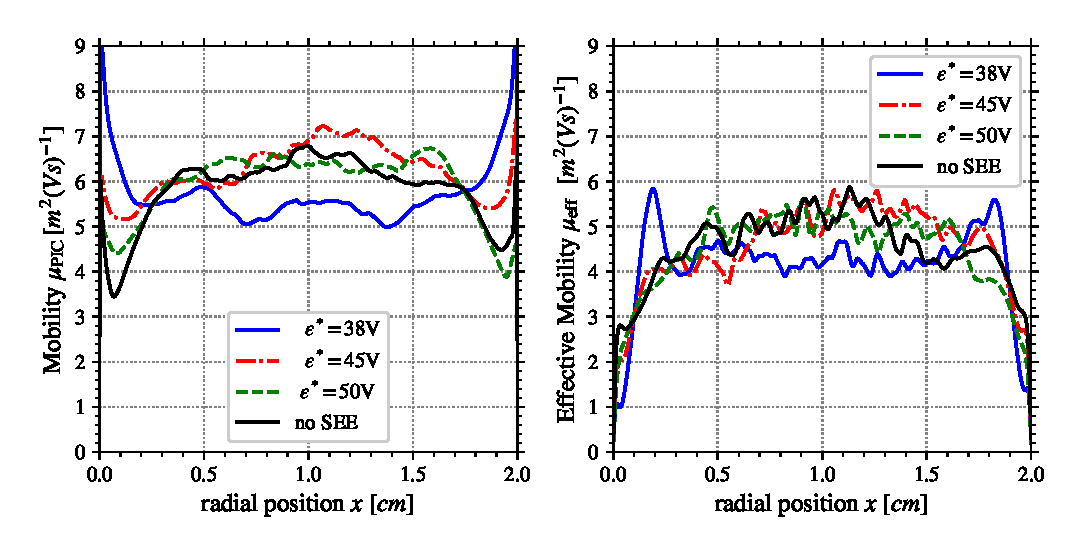
\includegraphics[width=\textwidth]{both_Mobility_SEE}
    \caption{Radial profile the electron mobility (left) measured in the \ac{PIC} simulations, and (right) given by \cref{eq-defmobeff}, for different wall emissivities. }
    \label{fig-radial-data}
  \end{figure}
  
  We can see in \cref{fig-radial-data} that the mobility measured $\mobpic$  in the center decreases by roughly 20\% as the emission rate increases.
  This observation is in agreement with $\mobeffsat$ observed in \cref{fig-radial-data,fig-mob-epsstar}.
  This is due the electron temperature $\Te$ which decreases from around $\Te=45$V at $\crover=200$V to $\Te=30$V at low $\crover$ (the evolution of $\Te$ can be seen in \cref{fig-Tevsproba}).
  
  On the other hand, the near wall mobility increases significantly on $\mobpic$ (almost by a factor of 2) with the increase of the electron emission.
  However, we do not see this evolution on $\mobeffsat$, meaning that it indeed comes from another physical mechanism than the \ac{ECDI}.
  
  
  \subsection{Three different regimes}
  \label{subsec-regimes}

  In \Cref{fig-mob-epsstar}, three regimes have been identified.
  Regime {\bf I} corresponds to low values of $\crover$ (lower than 35V), during which $\mobeffsat$ increases with $\crover$ but $\mobpic$ and $\mobeff$ decreases.
  Regime {\bf III} corresponds to high values of $\crover$ (higher than 50V), during which $\mobeffsat$, and  $\mobpic$ are roughlty constants, but $\mobeff$ increases slightly.
  Regime {\bf II} is a short transition regime, for $35 < \crover < 50$V.
  
  The different regimes are actually obvious when looking at the temporal evolution of the different variables.
  \Cref{fig-threeregimes}  presents the temporal evolution of the space average $\ratepic$ for three different
  values of $\crover$ , corresponding to three different regimes we have identified.
  In regimes {\bf I} and {\bf III}, $\ratepic$ reaches a steady state after a few microseconds.

  \begin{figure}[hbtp]
    \centering
    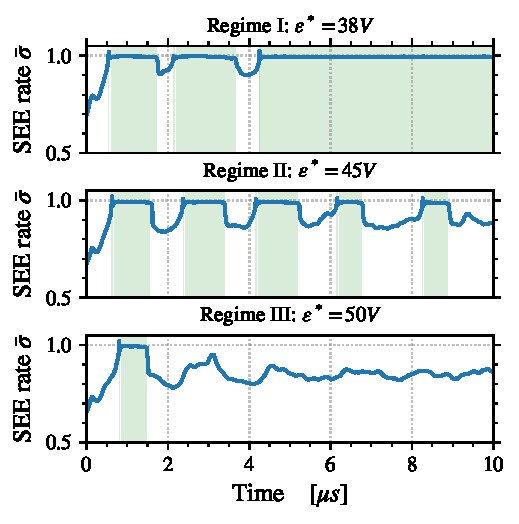
\includegraphics[width=\defaultwidth]{comparaison_3_regimes}
    \caption{Evolution as a function of time of the averaged electron emission rate $\ratepic$ in the three regimes observed (two stables, one with oscillations). The light green zones correspond to the periods when $\ratepic > \ratecr$}
    \label{fig-threeregimes}
  \end{figure}
  

  Regime {\bf I}, with low $\crover$, is characterized by a saturation of $\ratepic$ at a value between $\ratecr$ and 1, which leads to a non-monotonic potential profile.
  Regime {\bf III}, for higher $\crover$, is characterized by a steady state with a SEE rate lower than $\ratecr$.

  The transition between these two stable regimes (monotonic and non-monotonic sheath) passes by regime {\bf II}, an oscillating mode between the two stable regimes.
 As shown in \cref{fig-mob-epsstar}, regime {\bf II} is observed only in a narrow range of $\crover$.
 The oscillations of regime {\bf II} are shown in \cref{fig-threeregimes} up to $10\mus$ but have been observed for more than $40\mus$.
 Note that regimes {\bf I} and {\bf III} in \cref{fig-threeregimes} are obtained for $\crover = 38$~V and $\crover = 50$~V respectively, i.e. near the boundary of the unstable window (see \cref{fig-mob-epsstar}).
 Consequently, we observe a few oscillations before the steady-state is reached, as these cases are close to the bifurcation.
   
   
   The physical origin of the bifurcation can bee seen with the help of \cref{fig-dphivsTe}, which shows the evolution of the potential drop to the wall as a function of the electron temperature.
   It is computed using \cref{eq-seemaxw} for $\rate$ and \cref{eq-sheathhobbs} for the potential drop, which is summarized as 
   \begin{equation} \label{eq-dphi_vs_Te_Maxw}
     \begin{cases}
       \rate = \proba_0 + (1- \proba_0) \frac{2 \Te}{\crover} \\
       \dphi = \Te \ln \lp [1 - \rate] \sqrt{ \frac{m_i}{2 \pi m_e}}  \rp
     \end{cases}
   \end{equation}

   \begin{figure}[hbtp]
     \centering
     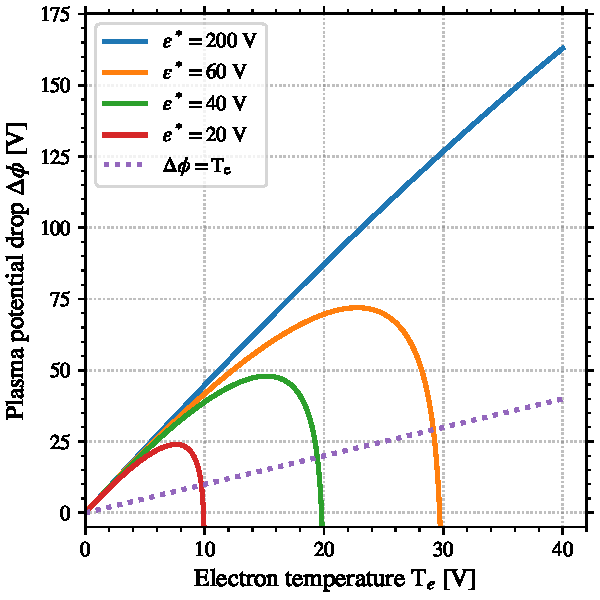
\includegraphics[width=\defaultwidth]{RSO_theo_sheath_bis}
     \caption{Plasma potential drop to the wall as a function of the electron temperature for different values of the cross-over energy $\crover$ using \cref{eq-dphi_vs_Te_Maxw}. The dashed line is $\dphi=\Te$. }
     \label{fig-dphivsTe}
   \end{figure}
   
   \Cref{fig-dphivsTe} shows the evolution of $\dphi$ as a function of $\Te$ obtained with \cref{eq-dphi_vs_Te_Maxw} using four different values of $\crover$. 
   We can see that, starting from low electron temperature, the potential drop increases with the electron temperature, resulting in a better screening of the electrons.
   This corresponds to regime {\bf III}.
   However, the $\dphi$ reaches a maximum, after which it drops sharply to zero and below.
   
   When the potential passes the maximum, the electrons are not screened by the sheath any more.
   Hence, the electrons reach the wall with a higher energy, resulting in a higher electron emission from the wall, hence a smaller potential drop.
   The sheath is unstable, and quickly attains a \ac{SCL} regime \citep{raitses2005}.
   
   In this regime, the sheath is not monotonic, and the model of \cref{eq-sheathhobbs} is no more valid, and the potential drop tends toward $\dphi \simeq \Te$ \citep{hobbs1967,goebel2008} \footnote{see \cref{sec-sheath} for more details}, shown in \cref{fig-dphivsTe}.
   This corresponds to regime {\bf I}.
   
   However, during regime {\bf I}, the electron power losses to the wall are very high, and they can exceed the gains.
   Hence, the electron temperature decreases.
   If $\Te$ decreases too much, the sheath can come back to the previous regime {\bf III}.
   The oscillations between regime {\bf I} and {\bf III} defines regimes {\bf II}.
      
   We have seen in \ref{fig-canon_Te_all} that without electron emission, $\Te$ is of the order of $45$~V.
   Using \cref{fig-dphivsTe}, we can expect to observe the transition between regime {\bf III} and {\bf II} for $\crover \gtrsim 60$~V, as for $\crover = 60$~V, the maximum of $\dphi$ is at $\Te\sim 25$~V, which is significantly lower than 45~V.
   The fact that regime {\bf II} appears at $\crover=50$~V can be explained because
   \begin{enumerate}
     \item a lower $\crover$ increases the electron losses, hence decreases the electron temperature at equilibrium,
     \item the electrons are not Maxwellian.
   \end{enumerate}
   
   The evolution of the temperature with $\crover$ is shown in \cref{fig-Tevsproba}.
   We can see that $\Te \simeq 45\,\volt$ for emission rate up to $\sigma = 0.8$, and decreases down to $\Te=30\,\volt$ for higher emission rates.
   Consequently, even if $\Te$ does indeed decreases when increasing $\crover$, it remains too large compared to the observations of \cref{fig-dphivsTe}.
   The impact of second point will be studied in \cref{ch-3}.
   
   
  
% !TEX root=/home/tavant/these/manuscript/src/manuscript.tex

\section{Validation of the sheath model }
  \label{sec-sheath_validation}
  
  The \ac{PIC} simulations used here do not need any sheath theory in order to model the plasma-wall interaction.
  Conversely, they rely on first principle models.
  Hence, they can be used in order to validate the sheath model introduced in \cref{sec-sheath} coming from the fluid theory.
  
  This sheath model links with \cref{eq-dphi_vs_Te_Maxw} the plasma potential drop $\dphi$ with the electron temperature $\Te$ and the electron emission rate $\rate$.
  \Cref{eq-seemaxw} can be used to estimate the electron emission rate given the mean electron temperature measured in the simulations, corresponding statistically to the plasma bulk temperature.   
  In the \ac{PIC} simulations, $\rate$ can be computed using \cref{eq-seeyield} by counting the number of electrons attaining the wall and emitted during a time-step.
  We note \ratepic this measurement.
  \vspace{1em}
   
  \begin{figure}[hbt]
    \centering
    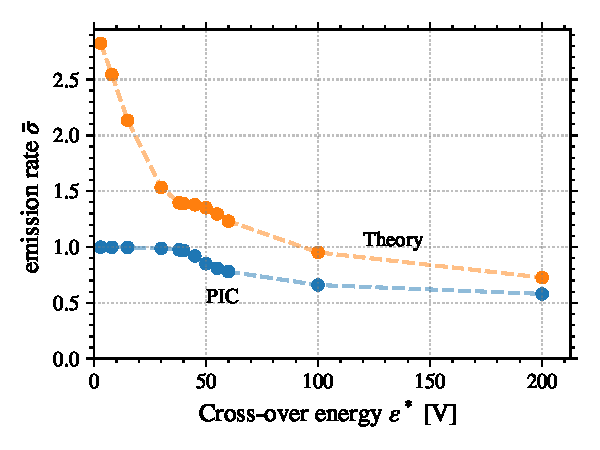
\includegraphics[width=\defaultwidth]{SEE_rates}
    \caption{Values of the electron emission rate $\ratepic$ (blue) measured in the \acs{PIC} simulations, and $ \ratemaxw$ obtained with \cref{eq-seemaxw} using the electron temperature shown in \cref{fig-Tevsproba}. }
    \label{fig-seeparamesMaxw}
  \end{figure}
  
  
  We can see in \Cref{fig-seeparamesMaxw} that the mean electron emission rate lies between 0.6 for large $\crover$ and 1 at low $\crover$.
  The saturation of $\ratepic$ at 1 for high emissivity ( $\crover < 50 \volt$) was not expected from \ratemaxw.
  Indeed, $\probamax$ is equal to 2.9, and the electron temperature in the bulk measured, when used in \cref{eq-seemaxw}, predicts a rate between 1.4 and 2.8.
  This discrepancy at low $\crover$ is due to the \ac{SCL} regime.
  \citet{hobbs1967} predicted that in this regime, a potential well forms such that a fraction of the emitted electrons return to the wall, in order to maintain the effective emission rate to $\ratecr\sim1$.
  However, for $\crover > 50 \volt$, the sheath regime described in \cref{sec-sheath} should be valid.
   
  \begin{figure}[hbt]
    \centering
    \begin{tabular}{@{} cc}
      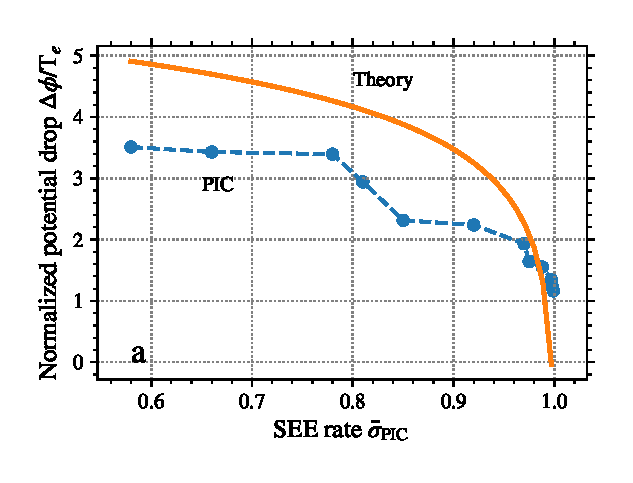
\includegraphics[width=0.45\textwidth]{phi_drop_6}
      &
      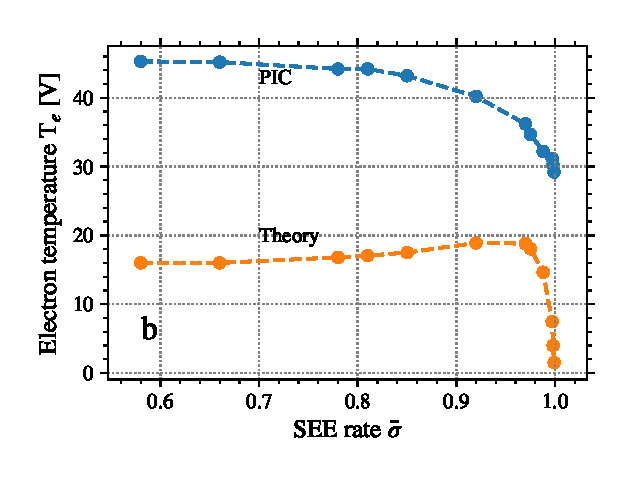
\includegraphics[width=0.45\textwidth]{Te_pic_2}
    \end{tabular}
    \caption{({\bf a}) Plasma potential drop to the wall normalized by the electron bulk temperature as a function of the electron rate, and ({\bf b}) the mean electron bulk temperature measured in the \acs{PIC} simulations as a function of the electron emission rate \rate, measured in the simulations, and the effective temperature expected from \cref{eq-Teeff}.  }
    \label{fig-Tevsproba}
  \end{figure}
  
  The electron temperature measured in the bulk of the simulation is presented in \cref{fig-Tevsproba}.{\bf b} for the same cases as in \cref{fig-seeparamesMaxw}.
  An \emph{effective} temperature that would correspond to the measured emission rate $\ratepic$ in \cref{eq-dphi_vs_Te_Maxw},
  \begin{equation} \label{eq-Teeff}
     \ratemaxw(\Te{}_{, eff}) = \ratepic \text{, hence } \Te{}_{, eff} = \frac{\ratepic - \sigo}{1 - \sigo} \frac{\crover}{2},
  \end{equation}
  is also given.
  We can see that when \rate increases, the electron temperature in the bulk $\Te$ monotonically decreases from 45V to around 30V.
  However, these values are not consistent with the measured emission rate \ratepic, even for $\crover > 50\volt$.
  The bulk electron temperature is much higher than the effective $\Te{}_{, eff}$ obtained to correctly predict the emission rate.

  \Cref{fig-Tevsproba}.{\bf a} shows the evolution of the potential drop to the wall measured in the \ac{PIC} simulation compared to the theory  \cref{eq-sheathhobbs} ).
  As expected by \cref{eq-dphi_scl}, $\dphi$ measured in the simulation saturates to $\Te$ for high emission rate ($\ratepic \sim 1$).
  However, we see that at low emission rate, the potential drop is significantly lower than expected.
  The sheath model of \cref{sec-sheath} used two hypotheses\string:
  \begin{itemize}
    \item Maxwellian distribution function to obtain $\ratemaxw$ from \cref{eq-seeyield},
    \item Isothermal electrons in the sheath.
  \end{itemize}
  These two hypotheses will be checked against the PIC simulations in the next chapter.

% !TEX root=/home/tavant/these/manuscript/src/manuscript.tex

\section{Full dielectric model }
  \label{sec-fulldiel}
  
  We have observed the effects of the electron emission and the electrostatic boundary condition separately in \cref{sec-diel_layer,sec-see}, respectively.  
  In \Cref{sec-see}, we observed three regimes depending on the emission rate.
  At high emissivity, the sheath is space-charge limited, resulting in an inverse sheath.
  At low emissivity, we obtain the standard sheath model with electron emission.
  The transition between the regimes passes by a oscillating regime.
  
  In \Cref{sec-diel_layer} we observed that when there is no emission, the dielectric boundary condition for the potential does not change the simulation results.
  In this section, we investigate the interaction between the two characteristics of the dielectric walls, especially with a high emission rate.
  More precisely, regime {\bf II} is the most interesting, as it features a complex behavior.
  Hence, we use $\crover=45\,\volt$ to study the impact of the dielectric layer combined with the electron emission.
  
  The dielectric layer thickness is $L_{\rm Diel} = 3\,\milli\meter$, and the relative permittivity of the dielectric is $\epsilon_R=25$.
  The dimensions of the plasma domain is not modified between the case with and without the dielectric layer.
  Instead, it is the width between the grounded electrodes that is increased.
  
  \subsection{Impact of the dielectric boundary condition on the mobility with electron emission}
    
    \Cref{fig-temporal_mu} shows the temporal evolution of the electron mobility measured in the simulation $\mobpic$ for both cases, with and without the dielectric layer.
    We can see that the two variables are quite similar, with similar mean values and oscillation.
    Interestingly, the beginning of the simulations, up to $t=3\,\micro\second$, are almost identical.
    After this, the values are not in phase.
    
    \begin{figure}[hbt]
      \centering
      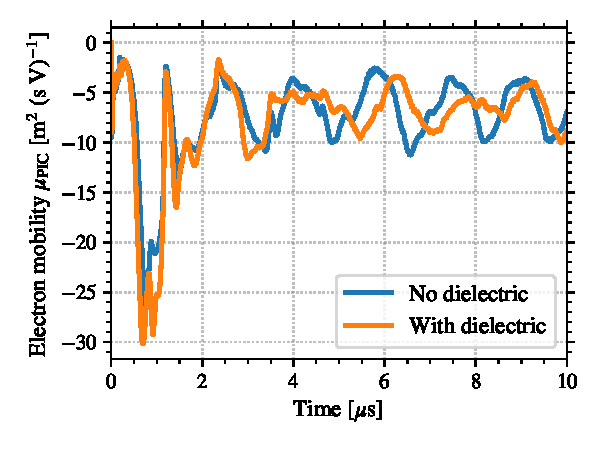
\includegraphics[width=\defaultwidth]{dielectron_yesSEE_mobility}
      \caption{Temporal evolution of the axial electron mobility measured in the \acs{PIC} simulation with and without the dielectric layer between the plasma and the grounded electrodes. The crossover energy is $\crover=45\,\volt$, the length of the dielectric layer is $L_{\rm Diel}=3\milli\meter$ and its relative permittivity is $\epsilon_R = 25$.  }
      \label{fig-temporal_mu} 
    \end{figure}
    
    
    \subsection{Plasma-wall interaction}

  
  \begin{figure}[hbt]
    \centering
    \begin{tabular}{@{} c c}
      \subfigure{see_diel_temporal}{a}{20,20} & 
      \subfigure{see_diel_space}{b}{20,20}
    \end{tabular}
    \caption{Comparison of the ({\bf a}) temporal and ({\bf b}) spatial evolution along the dielectric surface of the radial electric field at the wall calculated in PIC simulations compared to the electric field derived from the surface charge. }
    \label{fig-seediel_Er}
  \end{figure}
  \inlinenote{Anne: pas clair le choix des echelles de temps... Refaire ces figures avec les nouveaux resultats}
   
  \Cref{fig-seediel_Er} shows the ({\bf a}) temporal and ({\bf b}) spatial evolution along the dielectric surface of the radial electric field at the wall calculated in PIC simulations compared to the electric field derived from the surface charge, similarly  to \cref{fig-spacial_comparaison}.
  We can see that in contrast to the results of \cref{sec-diel_layer}, the two values are significantly different.
  The electric field measured in the \ac{PIC} simulation is rather uniform and constant, compared to the electric field at the surface calculated only based on the surface charge.
  Moreover, in \cref{fig-seediel_Er}.{\bf a}, we see that at around $t=2.1\,\second$, the electric field sign changes, meaning that the sheath passes from the \ac{SCL} regime {\bf I} to the normal regime {\bf III}, which is typical of regime {\bf II}.
  In contrast, the electric field derived from the surface charge does not shows this change of sheath regime.
  
  
  \begin{figure}[hbt]
    \centering
    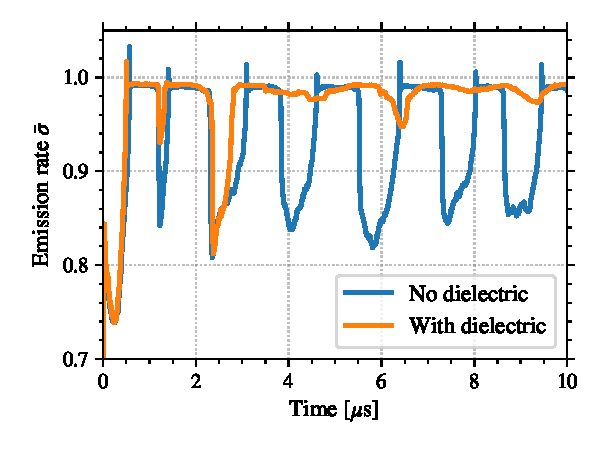
\includegraphics[width=\defaultwidth]{dielectron_yesSEE_SEErate}
    \caption{Temporal evolution of the mean electron emission rate $\ratepic$ for the same parameter $\crover=45\,\volt$, with and without the dielectric layer modeled.}
    \label{fig-rso_diel}
  \end{figure}
  
  \cref{fig-rso_diel} compares the temporal evolution of the mean electron emission rate $\ratepic$ for the same parameter $\crover=45\,\volt$, with and without the dielectric wall modeled.
  As previously, the dielectric width is $3\,\milli\meter$, and the electrodes are now $2.6\,\centi\meter$ apart (the geometry of the plasma domain is kept constant).
  We see that the oscillations occur for the two models.
  However, we can observe several differences.
  The first is the lower level of emission rate.
  When the walls are grounded, $\ratepic$ decreases at around $85\%$.
  Conversely, with the dielectric layer included, the emission rate does not decrease much below $95\%$.
  This results in a different overall mean emission rate, that can affect the particle and power balances, hence the mean electron temperature and the performance of the thruster.
  
  
  
  
  
% !TEX root=/home/tavant/these/manuscript/src/manuscript.tex

\section{Conclusion of the parametric study}
  \label{sec-conclusion_ch2}
  
  Using the \ac{PIC} simulation code introduced in \cref{ch-1}, we studied the effects of the dielectric walls on the discharge, and more precisely the effects on the electron axial mobility.
  To begin with, a \emph{base} case with metallic walls was defined and studied.
  The metallic walls correspond to grounded and non-emissive walls.
  For this reference case, we observed that the convection model used allows us to obtain a quasi steady-state.
  We observed an enhanced electron transport transverse to the magnetic field lines, because of the azimuthal instability.
  Both effects of the dielectric -- the electron induced electron emission and the electrostatic boundary condition -- were investigated.
  First, we  only modeled the dielectric boundary condition. Then, we studied only the electron emission. Afterwards, the two phenomena have been studied together.
  
  \subsubsection*{Electrostatic boundary condition}
  
  The electrostatic boundary condition is modeled by including in the domain of simulation the thickness of the wall ($L_{\rm Diel} = 3 \milli\meter$).
  Surface charges accumulate at the interface between the plasma and the wall.
  We observed that the modified boundary condition did not modify significantly the discharge and the axial cross-field electron mobility.
  Moreover, we saw that the boundary condition used results in a radial electric field $E_r$ of the same order of magnitude than the Neumann boundary condition of \cref{eq-neuman} but the spatio-temporal evolution is not identical.
  
  Indeed, when the secondary electron emission is modeled, the surface charges oscillates significantly compared to the radial electric field during the \ac{SCL} regime.
  As the dielectric model used here do not increase significantly the computational time, we recommend to use it instead of the Neumann boundary condition, that do not reproduce the same plasma-wall interaction.
  
  
  \subsubsection*{Electron induced electron emission}
  
  The electron  emission from the wall due to the impact of primary electron reaching the wall is modeled using the model described in \cref{sec-seemodel}.
  The value of the crossover energy $\crover$ is varied from a large value (low emissivity) to small values (high emissivity).
  We observed in the simulations that when the electron emission rate increases, the mean electron temperature decreases.
  This decreases the amplitude of the \ac{ECDI} at saturation, hence decreases the electron mobility in the plasma (see \cref{fig-radial-data}).
  However, electron emission induces \ac{NWC}, which almost doubles the electron mobility close to the wall when $\crover$ varies from $200\volt$ to $30\volt$.
  Consequently, the overall electron cross-field mobility is almost constant in our simulation.
  
  We observed in our \ac{PIC} simulations three different regimes depending on the values of $\crover$.
  For high values of $\crover$, the plasma stabilises with an emission rate $\ratepic < \ratecr$.
  When $\crover$ is small, we observe a stable configuration with $\ratepic \sim \ratecr$.
  Under these conditions, the sheath is space-charge limited.
  The transition between the two regimes is not stable, but instead passes by a bi-stable regime.
  In this third regime, the sheath jumps between the two stable regimes.
  

  \subsubsection*{Inconsistent sheath model }
  
  The simulation results have been compared to the sheath model of \citet{hobbs1967}.
  We observed a significant discrepancy between the \ac{PIC} simulations and the sheath model that comes from a fluid approach.
  In particular, the potential drop and the electron emission rate are both overestimated.
  These overestimations can lead to erroneous conclusion and prediction when using fluid models.
  Hence, a better understanding of the plasma-wall transition via the sheath is needed.
  
  The sheath model currently used is based mainly on two hypothesis
  \begin{itemize}
    \item Maxwellian electron distribution function
    \item Isothermal electrons in the sheath
  \end{itemize}
  
  Both hypotheses will be questioned in the next chapter.
  


% \acresetall
% !TEX root=/home/tavant/these/manuscript/src/manuscript.tex




\chapter{Anisothermal sheath}
\label{ch-3}

In order to explain the discrepancy observed in \cref{ch-2} between the simulation and the sheath model, we investigate the simulation data.
We see that the hypothesis of the sheath model do not stand.
Using a simplified \ac{1D} \ac{PIC} simulation, we derive a polytropic closure for the electron.
With this new closure equation, we derived a modified sheath model, that fit well the kinetic simulations. 


{\bf III. Polytrotic sheath model} 23 pages
\begin{zzz}
  This chapter takes the 2nd paper about the modified sheath model

  3.1 EVDF in the 2D PIC simulations of HET.    3 pages

  3.2 1D simplified simulations, Parametric study and polytropic fits. 7 pages

  3.3 Monte-Carlo simulations.  3 pages

  3.4 fluid equations with polytropic closure. 10 pages
\end{zzz}


\minitoc




% !TEX root=/home/tavant/these/manuscript/src/manuscript.tex



\section{Insights for the PIC simulations}
\label{sec-insights}

As announced in \vref{sec-sheath_validation}, the sheath model of \vref{sec-sheath} uses two hypothesis\string:
\begin{itemize}
  \item Maxwellian electrons,
  \item Isothermal evolution of the electrons.
\end{itemize}

When collisions can be neglected, as it is usually assumed in the sheath, these two hypothesis are linked.
Indeed, the \ac{1D} Maxwellian distribution function expressed as the total energy is
\begin{equation} \label{eq-maxw_total}
  f(\ek, \phi) \propto \exp \lp \frac{\ek - \phi}{\Te}  \rp = \propto \exp \lp \frac{\ek}{\Te} \frac{-\phi}{\Te},
\end{equation}
where $\ek$ and $\Te$ are the electron kinetic energy and temperature expressed in Volt.
We can see in \cref{eq-maxw_total} that the spatial variation (due to the plasma potential $\phi$) only affect the amplitude of the distribution function, not its shape in the energy space.
Hence, the electron temperature is uniform, i.e. they are isotherm.
In addition, we find that $n_e \propto \exp (- \phi / \Te)$, which is the definition of Boltzmann electrons.

Hence, let see if this two aspects are respected in the \ac{2D} \ac{PIC}-\ac{MCC} simulation results

\subsection{Electron distribution function}

\begin{figure}[hbtp]
  \centering
  \includegraphics[width=\defaultwidth]{EEDF_2-eps-converted-to}
  \caption{Electron energy distribution function of the electrons ({\bf a}) in the bulk, in the three directions, and ({\bf b}) in the bulk and in the sheath}
  \label{fig-EEDF}
\end{figure}

Using the kinetic information of the PIC simulations, we present in \Cref{fig-EEDF} the mean electron energy probability functions (EEPF) in the case $\crover = 200\,\volt$.
\Cref{fig-EEDF}.{\bf a} shows the projections of the EEPF in the centre of the simulations along the three directions.
These projections are compared to the Maxwellian probability function of the same
kinetic temperature.
\Cref{fig-EEDF}.{\bf b} shows the total EEPF for both the bulk and the sheath populations.
 The sheath length is defined as the location where the ions reach the Bohm speed, which is about 0.4mm.
 
 We see in \cref{fig-EEDF}.{\bf a} that the electron distribution function is not Maxwellian.
 In particular the high energy tails are depleted.
 However, we can see that the electrons are rather isotropic, compared to \ac{1D} simulation \citep{sydorenko2006}.
 In order to evaluate the effect of the nonMaxwellian EEPF, we numerically integrate the EEPF from the PIC data using \vref{eq-ratedifinition_evdf}.
The results (not shown) do not differ significantly from the Maxwellian values of \vref{eq-seemaxw}.
Hence, we can conclude that even if the Maxwellian hypothesis is not respected in the
PIC simulations, it is not enough to explain the differences observed in \vref{fig-seeparamesMaxw}.


\Cref{fig-EEDF}.{\bf b} presents the EEPF for the bulk population as well as for the sheath population.
 We can see that the sheath population is colder than the population at the centre, which could explain the difference of \vref{fig-seeparamesMaxw}. 
 This effect is assessed in the next section.



 


% \acresetall
\appendix

% \bibliographystyle{ieeetr}
\bibliographystyle{unsrtnat}  % for clever inline references
\bibliography{bib/MyLibrary}{}


%%%%%%%%%%%%%%%%%%%%%%%%%%%%%%%%%%%%%%%%%%%%%%%%%%%%%%%%%%%%%%%%%%%%%%%%%%%%%%%%%%%%%%%%%%%%%%%%%%%%%%%%%%%%%%%%%%%%%%%%%%%%%%%%%%%%%%%%%%%%%%%%%%%%%%%%%%%%%%%%%%%%%%%
%%%%%%%%%%%%%%%%%%%%%%%%%%%%%%%%%%%%%%%%%%%%%%%%%%%%%%%%%%%%%%%%%%%%%%%%%%%%%%%%%%%%%%%%%%%%%%%%%%%%%%%%%%%%%%%%%%%%%%%%%%%%%%%%%%%%%%%%%%%%%%%%%%%%%%%%%%%%%%%%%%%%%%%
%%% Modèle pour la 4ème de couverture des thèses préparées à l'Université Paris-Saclay, basé sur le modèle produit par Nikolas STOTT / Template for back cover of thesis made at Université Paris-Saclay, based on the template made by Nikolas STOTT
%%% Mis à jour par Aurélien ARNOUX (École polytechnique)/ Updated by Aurélien ARNOUX (École polytechnique)
%%% Les instructions concernant chaque donnée à remplir sont données en bloc de commentaire / Rules to fill this file are given in comment blocks
%%% ATTENTION Ces informations doivent tenir sur une seule page une fois compilées / WARNING These informations must contain in no more than one page once compiled
%%%%%%%%%%%%%%%%%%%%%%%%%%%%%%%%%%%%%%%%%%%%%%%%%%%%%%%%%%%%%%%%%%%%%%%%%%%%%%%%%%%%%%%%%%%%%%%%%%%%%%%%%%%%%%%%%%%%%%%%%%%%%%%%%%%%%%%%%%%%%%%%%%%%%%%%%%%%%%%%%%%%%%%
%%% Version du 19 juillet 2018 (Merci à Hadrien VROYLANDT (Univ. Paris-Sud) pour ses suggestions et corrections)
%%%%%%%%%%%%%%%%%%%%%%%%%%%%%%%%%%%%%%%%%%%%%%%%%%%%%%%%%%%%%%%%%%%%%%%%%%%%%%%%%%%%%%%%%%%%%%%%%%%%%%%%%%%%%%%%%%%%%%%%%%%%%%%%%%%%%%%%%%%%%%%%%%%%%%%%%%%%%%%%%%%%%%%

\documentclass[a4paper]{article}
\usepackage[utf8]{inputenc}
\usepackage{helvet}
\renewcommand{\familydefault}{\sfdefault}
\usepackage{geometry}
\geometry{
left=16mm,
top=30mm,
right=16mm,
bottom=30mm
}
\usepackage{xcolor}
\definecolor{bordeau}{rgb}{0.3515625,0,0.234375}
\usepackage[absolute,overlay]{textpos}
\usepackage{graphicx}
\usepackage{lipsum}
\usepackage{array}
\usepackage{caption}
\usepackage{multicol}
\setlength{\columnseprule}{0pt}
\setlength\columnsep{10pt}

\usepackage[french]{babel}

\label{form}
%%%%%%%%%%%%%%%%%%%%%%%%%%%%%%%%%%%%%%%%%%%%%%%%%%%%%%%%%%%%%%%%%%%%%%%%%%%%%%%%%%%%%%%%%%%%%%%%%%%%%%%%%%%%%%%%%%%%%%%%%%%%%%%%%%%%%%%%%%%%%%%%%%%%%%%%%%%%%%%%%%%%%%%
%%%%%%%%%%%%%%%%%%%%%%%%%%%%%%%%%%%%%%%%%%%%%%%%%%%%%%%%%%%%%%%%%%%%%%%%%%%%%%%%%%%%%%%%%%%%%%%%%%%%%%%%%%%%%%%%%%%%%%%%%%%%%%%%%%%%%%%%%%%%%%%%%%%%%%%%%%%%%%%%%%%%%%%
%%% Formulaire / Form
%%% Remplacer les paramètres des \newcommand par les informations demandées / Replace \newcommand parameters by asked informations
%%%%%%%%%%%%%%%%%%%%%%%%%%%%%%%%%%%%%%%%%%%%%%%%%%%%%%%%%%%%%%%%%%%%%%%%%%%%%%%%%%%%%%%%%%%%%%%%%%%%%%%%%%%%%%%%%%%%%%%%%%%%%%%%%%%%%%%%%%%%%%%%%%%%%%%%%%%%%%%%%%%%%%%
%%%%%%%%%%%%%%%%%%%%%%%%%%%%%%%%%%%%%%%%%%%%%%%%%%%%%%%%%%%%%%%%%%%%%%%%%%%%%%%%%%%%%%%%%%%%%%%%%%%%%%%%%%%%%%%%%%%%%%%%%%%%%%%%%%%%%%%%%%%%%%%%%%%%%%%%%%%%%%%%%%%%%%%

\newcommand{\logoEd}{ed}																		%% Logo de l'école doctorale. Indiquer le sigle / Doctoral school logo. Indicate the acronym : 2MIB; AAIF; ABIES; BIOSIGNE; CBMS; EDMH; EDOM; EDPIF; EDSP; EOBE; INTERFACES; ITFA; PHENIICS; SDSV; SDV; SHS; SMEMAG; SSMMH; STIC
\newcommand{\PhDTitleFR}{titre (en français)}													%% Titre de la thèse en français / Thesis title in french
\newcommand{\keywordsFR}{3 à 6 mots clés}														%% Mots clés en français, séprarés par des , / Keywords in french, separated by ,
\newcommand{\abstractFR}{\lipsum[1-3]}															%% Résumé en français / abstract in french

\newcommand{\PhDTitleEN}{titre (en anglais)}													%% Titre de la thèse en anglais / Thesis title in english
\newcommand{\keywordsEN}{3 à 6 mots clés}														%% Mots clés en anglais, séprarés par des , / Keywords in english, separated by ,
\newcommand{\abstractEN}{\lipsum[1-3]}															%% Résumé en anglais / abstract in english

\label{layout}
%%%%%%%%%%%%%%%%%%%%%%%%%%%%%%%%%%%%%%%%%%%%%%%%%%%%%%%%%%%%%%%%%%%%%%%%%%%%%%%%%%%%%%%%%%%%%%%%%%%%%%%%%%%%%%%%%%%%%%%%%%%%%%%%%%%%%%%%%%%%%%%%%%%%%%%%%%%%%%%%%%%%%%%
%%%%%%%%%%%%%%%%%%%%%%%%%%%%%%%%%%%%%%%%%%%%%%%%%%%%%%%%%%%%%%%%%%%%%%%%%%%%%%%%%%%%%%%%%%%%%%%%%%%%%%%%%%%%%%%%%%%%%%%%%%%%%%%%%%%%%%%%%%%%%%%%%%%%%%%%%%%%%%%%%%%%%%%
%%% Mise en page / Page layout      
%%% NE RIEN MODIFIER / DO NOT MODIFY
%%%%%%%%%%%%%%%%%%%%%%%%%%%%%%%%%%%%%%%%%%%%%%%%%%%%%%%%%%%%%%%%%%%%%%%%%%%%%%%%%%%%%%%%%%%%%%%%%%%%%%%%%%%%%%%%%%%%%%%%%%%%%%%%%%%%%%%%%%%%%%%%%%%%%%%%%%%%%%%%%%%%%%%
%%%%%%%%%%%%%%%%%%%%%%%%%%%%%%%%%%%%%%%%%%%%%%%%%%%%%%%%%%%%%%%%%%%%%%%%%%%%%%%%%%%%%%%%%%%%%%%%%%%%%%%%%%%%%%%%%%%%%%%%%%%%%%%%%%%%%%%%%%%%%%%%%%%%%%%%%%%%%%%%%%%%%%%

\begin{document}
\pagestyle{empty}

%%% Logo de l'école doctorale. Le nom du fichier correspond au sigle de l'ED / Doctoral school logo. Filename correspond to doctoral school acronym
%%% Les noms valides sont / Valid names are : 2MIB; AAIF; ABIES; BIOSIGNE; CBMS; EDMH; EDOM; EDPIF; EDSP; EOBE; INTERFACES; ITFA; PHENIICS; SDSV; SDV; SHS; SMEMAG; SSMMH; STIC
\begin{textblock*}{61mm}(16mm,3mm)
	\noindent\includegraphics[height=24mm]{media/ed/\logoEd.jpeg}
\end{textblock*}



%%%Titre de la thèse en français / Thesis title in french
\begin{center}
\fcolorbox{bordeau}{white}{\parbox{0.95\textwidth}{
{\bf Titre:} \PhDTitleFR 
\medskip

%%%Mots clés en français, séprarés par des ; / Keywords in french, separated by ;
{\bf Mots clés:} \keywordsFR 
\vspace{-2mm}

%%% Résumé en français / abstract in french
\begin{multicols}{2}
{\bf Résumé:} 
\abstractFR 
\end{multicols}
}}
\end{center}

\vspace*{0mm}

%%%Titre de la thèse en anglais / Thesis title in english
\begin{center}
\fcolorbox{bordeau}{white}{\parbox{0.95\textwidth}{
{\bf Title:} \PhDTitleEN 

\medskip

%%%Mots clés en anglais, séprarés par des ; / Keywords in english, separated by ;
{\bf Keywords:}  \keywordsEN %%3 à 6 mots clés%%
\vspace{-2mm}
\begin{multicols}{2}
	
%%% Résumé en anglais / abstract in english
{\bf Abstract:} 
\abstractEN
\end{multicols}
}}
\end{center}


\begin{textblock*}{161mm}(10mm,270mm)
\color{bordeau}
{\bf\noindent Université Paris-Saclay	         }

\noindent Espace Technologique / Immeuble Discovery 

\noindent Route de l’Orme aux Merisiers RD 128 / 91190 Saint-Aubin, France 
\end{textblock*}

\begin{textblock*}{20mm}(182mm,255mm)
\includegraphics[width=20mm]{media/UPSACLAY-petit}
\end{textblock*}

\end{document}

\end{document}
